\documentclass[12pt]{article}

%Technometrics specified margins:

% NOTE: To produce blinded version, replace "0" with "1" below.
\newcommand{\blind}{1}

% DON'T change margins - should be 1 inch all around.
\addtolength{\oddsidemargin}{-.5in}%
\addtolength{\evensidemargin}{-.5in}%
\addtolength{\textwidth}{1in}%
\addtolength{\textheight}{1.3in}%
\addtolength{\topmargin}{-.8in}%
\usepackage{psfrag,epsf,enumerate}

%\usepackage[margin=1.1in]{geometry}
\usepackage{color, amssymb, amsmath,bm,verbatim}
\usepackage{rotating, subfig, setspace, tikz}
\usepackage{graphicx, graphics, epsfig}
\usepackage{multirow,multicol}
\usepackage{natbib}
\newcommand{\tr}{{\mathbf{tr}}}
\newcommand{\rmk}{{\mathcal{K}}}
\newcommand{\I}{{\mathrm{I}}}
\newcommand{\E}{{\mathrm{E}}}
\newcommand{\B}{{\mathcal{B}}}
\newcommand{\bmo}{{\bm{o}}}
\newcommand{\R}{{\mathbb{R}}}
\newcommand{\cov}{{\mathrm{Cov}}}
\newcommand{\Log}{\text{Log}}
\newcommand{\M}{\mathcal{M}}
\newcommand{\refeq}[1]{{eq.~(\ref{#1})}}

\newcommand{\ProjMean}{{\widehat{\bm S}_E}}
\newcommand{\ProjMedian}{{\widetilde{\bm S}_E}}
\newcommand{\GeomMean}{{\widehat{\bm S}_R}}
\newcommand{\GeomMedian}{{\widetilde{\bm S}_R}}
\newcommand{\Rdist}{{d_R}}
\newcommand{\Edist}{{d_E}}

\DeclareMathOperator*{\argmax}{arg\,max}
\DeclareMathOperator*{\argmin}{arg\,min}
\newcommand{\blue}[1]{{\color{blue} #1}}
\newcommand{\red}[1]{{\color{red} #1}}
\newcommand{\green}[1]{{\color{green} #1}}
\newcommand{\hh}[1]{{\color{orange} #1}}

%\pagestyle{plain}
%\bibliographystyle{plainnat}
\bibliographystyle{abbrvnat}
\setcounter{section}{0}
\bibpunct{(}{)}{;}{a}{,}{;}
\graphicspath{{images/}}
%\setlength{\parindent}{0pt}
\begin{document}

\def\spacingset#1{\renewcommand{\baselinestretch}%
{#1}\small\normalsize} \spacingset{1}

\if0\blind
{
  \title{\bf Point Estimation of the Central Orientation of Random Rotations}
  \author{Bryan Stanfill\\
    Ulrike Genschel \\
    and\\
    Heike Hofmann\\
    Department of Statistics, Iowa State University\\}
  \maketitle
} \fi

\if1\blind
{
  \bigskip
  \bigskip
  \bigskip
  \begin{center}
    {\LARGE\bf Point Estimation of the Central Orientation of Random Rotations}
\end{center}
  \medskip
} \fi

%\title{Point Estimation of the Central Orientation of Random Rotations}
%\author{Bryan Stanfill, Ulrike Genschel, Heike Hofmann}
%\date{\today}


%\begin{comment}
\bigskip
\begin{abstract}
%\footnotesize
Data as three-dimensional rotations have application in computer science, kinematics and materials sciences, among other areas.  Estimating the central orientation from a sample of such data is an important problem, which is complicated by the
fact that several different approaches exist for this,  motivated by various geometrical and decision-theoretic considerations. However, little is known about how such estimators compare, especially on common distributions for location models with random rotations.  We examine four location estimators, three of which are commonly found in different literatures and the
fourth estimator (a projected median) is newly introduced.  Our study unifies
existing literature and provides a detailed numerical investigation of location estimators for three commonly used rotation distributions in statistics and materials science.  While
the data-generating model influences the best choice of an estimator, the proposed projected median emerges as an overall good performer, which can be suggested
without particular distributional assumptions.  We illustrate the estimators 
and our findings with data from a materials science study by approximating the central orientation of cubic crystals on the micro-surface of a metal. Accompanying supplemental materials are available online.


\noindent\textit{Keywords}: Cayley distribution, Electronic Backscatter Diffraction, Geodesic distance, Matrix Fisher distribution, Projected median,  Rotation Group \end{abstract}
%\end{comment}
\spacingset{1.45} % DON'T change the spacing!
%\doublespace
\newpage
 % !TEX root = Stanfill_CoDA.tex
\section{Introduction}\label{ch:intro}

Data in the form of $3 \times 3$ rotation matrices find application in several scientific areas, 
such as biomedical engineering, computer visioning, and geological and materials sciences, where such data represent the positions of objects within some three-dimensional
reference frame.  For example, \citet{rancourt00} examine rotation matrix data in studying body 
positions whilst operating machinery. \cite{fletcher09} consider this type of  orientation data in 
magnetic resonance imaging and in shape analysis; similar examples  can be found in \cite{schwartz05}, \cite{pierrynowski09},  \cite{dai10},  or \cite{hadani11}.  The data in our illustrative 
example to follow arise from a study in materials science, where $3 \times 3$ rotations represent the orientations of cubic crystals on the micro-surface of a metal specimen as measured through electron backscatter diffraction (EBSD) and ``grains" within metals are composed of crystals which roughly share a common orientation; see \cite{randle03} for details on EBSD data.  
     
From a sample of orientations, an important interest is often the estimation of a main or central orientation $\bm S$.  That is, letting the rotation group $SO(3)$ denote the collection of all $3\times 3$ rotation matrices, observations $\bm{R}_1,\ldots,\bm{R}_n \in SO(3)$ can be conceptualized as a random sample from a \textit{location model}
\begin{equation}
\label{eqn:1}
\mathbf{R}_i = \bm{S} \bm{E}_i, \quad i=1,\ldots,n,
\end{equation}
where $\bm S \in SO(3)$ is the {\it fixed} parameter of interest indicating an orientation of central tendency, and $\bm{E}_1,\ldots,\bm{E}_n \in SO(3)$ denote i.i.d.{\it random} rotations which symmetrically perturb $\bm{S}$. The data-generating model in \eqref{eqn:1} is a rotation-matrix analog of a location model for scalar data $Y_i = \mu + e_i$, where $\mu \in \mathbb{R}$ denotes a mean and $e_i \in \mathbb{R}$ denotes an additive error symmetrically distributed around zero.  This representation \eqref{eqn:1} for orientations is quite common and, in fact,
a variety of parametric models exist for describing symmetrically distributed rotations $\bm{E}_i$, such as the symmetric matrix Fisher distribution \citep{downs72}, the symmetric Cayley distribution
\citep{leon06}  and the circular-von Mises-based rotation distribution \citep{bingham09}   in the statistics literature, as well as the Bunge distribution \citep{bunge82}, the isotropic Gaussian
distribution \citep{matthies88, savyolova95} and the de la Vall\'{e}e Poussin distribution \citep{Schaeben97} in the materials science literature. Our goal in this paper is to summarize and compare the most frequently proposed approaches for point estimation of $\bm S$ based on a sample of orientation data generated by \eqref{eqn:1}.  Depending on the scientific literature, the approaches can be quite different.

The topic of location estimation has received considerable attention for directional data on circles or spheres, \citep[see][]{fisher53, karcher77, khatri77, fisher85, ducharme87, bajaj88, liu92, chan93, mardia00}, but less is known about  estimator properties with rotation data.
As a compounding factor, several current approaches to estimating $\bm S$ have arisen out of literatures having differing statistical and geometrical emphases.  In the  applied sciences literature, estimators of $\bm S$ are typically based on
{\it non-Euclidean} (i.e., Riemannian) geometry, such as the \emph{geometric mean} \citep{arun87, horn88, umeyama91, moakher02} or, more recently, the \emph{geometric median} \citep{fletcher08, fletcher09}.
Preferences may depend on outliers in the data, but such suggestions for estimating $\bm S$
often do {\it not} consider the potential impact of the
underlying data-generating mechanism.   On the other hand,
approaches in the statistics literature tend to motivate an estimator for $\bm S$  through likelihood or moment-estimation principles applied to a specifically assumed distributional model (e.g., matrix Fisher or Cayley distribution) for the symmetric rotation errors $\bm E_i$ \citep{downs72, jupp79, leon06, bingham10}. Almost always, this estimator turns out to be 
a \emph{projected arithmetic mean} based on {\it Euclidean} geometry. Hence, in addition to potential distributional assumptions, more fundamental divisions in estimation approaches may be attributable to different geometrical perspectives with rotation data.  

Considering the potential effects of an underlying data generation model as well as the choice of geometry (i.e., Euclidean vs.~Riemannian), the above discussion indicates a need to investigate and identify good point estimators for rotation data.  In particular, because estimators in the applied sciences literatures  are often selected without decision-theoretical considerations based on underlying distributions, it is of interest to understand how different location estimators behave across common distributions for rotations.  In this paper, we evaluate four estimators for $\bm S$ in the context of the location model \eqref{eqn:1}. These are either mean- or median-type estimators and based either on Euclidean- or Riemannian geometry; the Euclidean-based median estimator is introduced for the first time for $SO(3)$ data. Its inclusion is natural and its performance can be generally quite good and is (as will be demonstrated) broadly recommendable.   Through simulation, we compare how these estimators perform with respect to three common probability models for symmetric rotation errors as defined in \eqref{eqn:1}, namely the circular-von Mises-based distribution, the symmetric matrix Fisher distribution and the symmetric Cayley distribution.  The matrix Fisher is arguably the most common distribution in the statistics literature \citep[see][]{chikuse03}. While not noted previously, the symmetric Cayley and the de la Vall\'{e}e Poussin distribution are in fact the same; the de la Vall\'{e}e Poussin distribution has been advocated in the material science literature \citep{Schaeben97}.   The circular-von Mises-based distribution is included because the distribution is non-regular and has been applied to EBSD data \citep{bingham09}.  We describe how error distribution assumptions for rotation data, in particular their variability and tail behavior, translate into performance differences among point estimators.\\

The remainder of the manuscript is organized  as follows.  Section~\ref{ch:bg} provides a brief background on the geometry of rotations and different distance metrics that can be used to assess overall estimation bias.   Section~\ref{sec:estimators} then describes the location estimators for rotation data  and compares their geometric underpinnings, which  serves to unify some of the existing estimation literature.  Section~4 explains the design of the simulation study followed by a summary of our main findings in Section~5. Section~6 provides an illustration of the estimation methods for EBSD data in a materials science application. We provide concluding remarks and future research possibilities in Section~7.

 % !TEX root = Stanfill_CoDA.tex
\section{Background}\label{ch:bg}
\subsection{Geometry of Three-dimensional Orientations}
\label{subsec:geometry}

Three-dimensional orientation data consist of  observations belonging to the group $SO(3)$, where an element $\bm R$ in $SO(3)$ is an orthogonal 
$3\times 3$ matrix (i.e., $\bm{R}^\top \bm{R}=\bm{I}_{3\times3}$) with
determinant one.  As $SO(3)$ is a Lie group, its elements live on a differentiable
manifold.  This fact is helpful in understanding the two different geometric approaches 
for estimating the central location $\bm{S} \in SO(3)$ from a sample of orientation data, referred to here 
as the \textit{intrinsic}  and  the \textit{embedding} estimation approaches (see also \citet{jupp89} and \citet{mardia00} for analogs with directional data).

\noindent The rotation group $SO(3)$ is not closed under routine addition or scalar multiplication (i.e., operations natural to statisticians). Hence, statistical estimation approaches often \textit{embed} the rotation group into the higher-dimensional linear space consisting of all $3\times 3$ real matrices, denoted as $\M(3)$.  Doing so enables the use of the familiar Euclidean geometry (and ``averaging'' notions) to define standard distance measures  and loss criteria for obtaining location estimators (see Section~\ref{subsec:metrics} and the estimators given in Sections \ref{subsec:pam} and \ref{subsec:med}).  This embedding technique has been largely  applied by statisticians, typically resulting in the projected arithmetic mean of Section~\ref{subsec:pam}.
See, for example, \cite{downs72, khatri77} and \cite{jupp79, jupp89}. The Bayesian estimator used in \cite{bingham10} is another concrete example of this
approach as is the median-type estimator we propose in Section~\ref{subsec:med}.

\noindent Alternatively, \textit{intrinsic} estimation approaches use Riemannian geometry to define distances that account for the innate topology or curvature of the space $SO(3)$.  In the intrinsic approach, each rotation from $SO(3)$ is
associated with a skew-symmetric matrix $\bm{\Phi}(\bm{W})$, defined  as
\[
  \bm{\Phi}(\bm{W}) = \left[ \begin{array}{ccc} 0 & -w_3 & w_2\\
  w_3 & 0 & -w_1\\
 - w_2 & w_1 & 0\\
  \end{array}
 \right]
\]
for $\bm{W}=(w_1, w_2, w_3)^\top \in \mathbb{R}^3$. That is, through a so-called exponential operator,
we map  $\bm{\Phi}(\bm{W})$ to a rotation matrix as
\[
  \exp[\bm{\Phi}(\bm{W})] = \sum\limits_{k=0}^\infty \frac{[\bm{\Phi}(\bm{W})]^k}{k!}=\cos(r)\bm{I}_{3\times3} + \sin(r) \bm{\Phi}(\bm{U}) + (1-\cos r) \bm{U} \bm{U}^\top
\]
where $r=\|\bm{W}\|$ and $\bm{U} =\bm{W}/\|\bm{W}\| $.  The space $\mathfrak{so}(3)$ of all skew-symmetric matrices forms the tangent space (Lie-algebra) of $SO(3)$, which is closed under familiar summation and scalar multiplication operations in the usual (i.e., element-wise) manner. The fact that $SO(3)$ is a differentiable manifold allows a distance measure (the geodesic distance in Section~\ref{subsec:metrics}) to be defined between points in $SO(3)$ according to Riemannian geometry. The resulting geodesic distance provides the basis for the ``geometric" location estimators commonly found in computer science \citep{fletcher08, fletcher09, hartley11} and engineering applications \citep{manton04}; see Sections~\ref{section:ltwo} and \ref{subsec:lone}.

\noindent Before leaving this section, it is helpful to note that each rotation matrix $\bm{R}$ can be associated with an angle-axis 
pair $(r,\bm{U})$, where $r\in(-\pi,\pi]$ and $\bm{U}\in\mathbb{R}^3$, $\|\bm{U}\|=1$, through
\begin{equation}
\label{eqn:angleaxis}
 \bm{R} = \bm{R}(r,\bm{U}) = \exp[\bm\Phi(\bm{U} r)] \in SO(3).
\end{equation}
This is Euler's axis-angle representation of $\bm{R}$, where $\bm{R}$ is represented by rotating the coordinate axis $\bm{I}_{3 \times 3}$ about the axis $\bm{U}\in\mathbb{R}^3$ by the angle $r$. In the materials science literature,
$\bm{U}$ and $r$ are commonly referred to as the misorientation axis and misorientation angle of $\bm R$ with respect to  $\bm{I}_{3 \times 3}$; see \cite{randle03}.


\subsection{Choice of Distance Metrics}\label{subsec:metrics}

The choice of geometry, i.e.~Riemannian or Euclidean, results in two different metrics to measure the distance
between two rotation matrices $\bm{R}_1$ and $\bm{R}_2 \in SO(3)$. Under the embedding approach, the natural distance
metric between two random matrices is the Euclidean distance, $\Edist $, which is induced by the Frobenius norm
\begin{equation}
\label{d_E}
\Edist (\bm{R}_1,\bm{R}_2)=\|\bm{R}_1-\bm{R}_2\|_F, 
\end{equation}
where $\|\bm{A}\|_F = \sqrt{\mathbf{tr}({\bm A^\top \bm A})}$ denotes the Frobenius norm of a matrix $\bm A$ and $\mathbf{tr}(\cdot)$ denotes the trace of a matrix.  The Euclidean distance between two rotation matrices corresponds to the shortest cord in $\M(3)$  that connects both matrices. (For an illustrative example of $\Edist (\bm{R}_1,\bm{R}_2)$, we refer to Figure~\ref{fig:dEvsdG} where $\Edist (\bm{R}_1,\bm{R}_2)$ corresponds to the gray line.)  If $r\in(-\pi,\pi]$ denotes the misorientation angle in the angle-axis representation (\ref{eqn:angleaxis}) of $\bm{R}_1^\top \bm{R}_2 \equiv \bm{R}_1^\top \bm{R}_2(r,\bm{U})$ (so that $\mathbf{tr}(\bm{R}_1^\top \bm{R}_2) =1 +2 \cos r$), then $\Edist (\bm{R}_1,\bm{R}_2) = 2\sqrt{2}\sin(|r|/2)$ holds (see the supplemental material online for a short proof of this).

\noindent By staying in the Riemannian space $SO(3)$ under the intrinsic approach, the natural distance metric becomes the Riemannian (or geodesic) distance, $\Rdist $, between two rotations $\bm{R}_1,\bm{R}_2\in SO(3)$ defined as
\begin{equation}
\label{d_R}
\Rdist (\bm{R}_1,\bm{R}_2)=  \frac{1}{\sqrt{2}}||
\Log(\bm{R}_1^\top\bm{R}_2)||_F = |r|,
\end{equation}
where $\Log(\bm{R})$ denotes the principle logarithm of $\bm{R}$ where $\Log(\bm{R})$ denotes the principle logarithm of 
$\bm{R}$  and $r\in(-\pi,\pi]$   is the misorientation angle of $\bm{R}_1^\top \bm{R}_2$. For more information on the definition and existence 
of $\Log(\bm{R})$ we refer to \cite{moakher02}.
The Riemannian distance corresponds to the length of the shortest path that connects $\bm{R}_1$ and $\bm{R}_2$ {\it within} the space $SO(3)$; see Figure~\ref{fig:dEvsdG} for an illustration. For this reason, the Riemannian distance is often considered the more natural metric on $SO(3)$; see \cite{moakher02} for this discussion along with more details on exponential and logarithmic operators related to $SO(3)$.    
 
%To exemplify the difference between the Euclidean and Riemannian distance metric, we visualize each distance in a lower dimensional example in Figure \ref{fig:dEvsdG}.  In Figure \ref{fig:dEvsdG} $\bm R_1,\bm R_2$ refer to the endpoints of two rotations on $SO(2)$.  The Riemannian distance between both rotations, $\Rdist (\bm R_1,\bm R_2)$,  corresponds to the thick curved line.  The rotation of $\bm R_1\bm v$ into $\bm R_2\bm v$ follows the curved path and therefore is considered to stay in the space.  The Euclidean distance between $\bm R_1,\bm R_2$, $\Edist (\bm R_1,\bm R_2)$, is represented by the straight gray line.  Because it is not possible for $\bm R_1\bm v$ to follow this straight path, the distance $\Edist (\bm R_1,\bm R_2)$ can only be obtained by leaving $SO(2)$.

\begin{figure}[h!]
\begin{center}
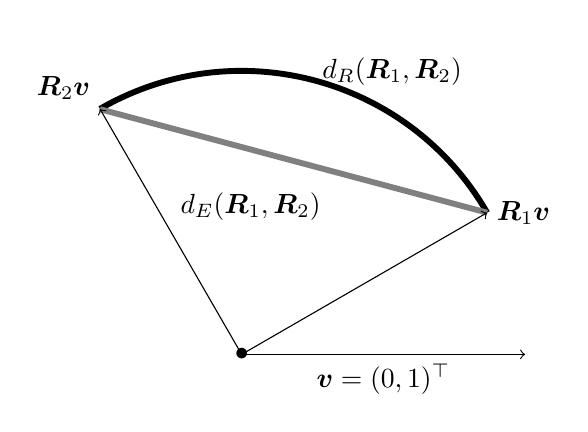
\begin{tikzpicture}[scale=.9]
%\draw (0,0) circle (4cm);
\draw (0,0) node {$\bullet$};
\draw (3.464102,2) node[anchor =  west]{$\bm R_1\bm v$};
\draw [->] (0,0)--(4,0);
%\draw [->] (4,0) arc (0:30:4cm);
\draw (2,0) node[anchor = north]{$\bm v=(0,1)^\top$};
\draw (-2,3.46) node[anchor = south east]{$\bm R_2\bm v$};
\draw [line width=.75mm] (3.464102,2) arc (30:120:4cm);
\draw[line width=.75mm, color=gray] (-2,3.46)--(3.464102,2);
\draw [->](0,0) -- (-2,3.464102);
\draw [->](0,0)--(3.464102,2);
\draw (1,3.66) node[anchor= south west]{$\Rdist (\bm R_1,\bm R_2)$};
\draw (-1,1.75) node[anchor= south west]{$\Edist (\bm R_1,\bm R_2)$};
%\draw (0,0) circle (4cm);
%\draw (0,0) node {$\bullet$};
%\draw (0,0)--(4,0) node[anchor =  west]{$o_1$};
%\draw (4,0) node[anchor =  west]{$\bm R_1$};
%\draw (0,0)--(-2,3.46) node[anchor = south east]{$o_2$};
%\draw (-2,3.46) node[anchor = south east]{$\bm R_2$};
%\draw[line width=.75mm] (4,0) arc (0:120:4cm);
%\draw[line width=.75mm, color=gray] (-2,3.46)--(4,0);
%\draw (0,0)--(2,3.46) node[anchor= south west]{$\alpha$};
%\draw (2,3.46) node[anchor= south west]{$\Rdist (\bm R_1,\bm R_2)$};
%\draw (-1.25,0.73) node[anchor= south west]{$\Edist (\bm R_1,\bm R_2)$};
%\draw (3/8,.7)[->] arc (60:120:.75cm);
%\draw (0,1.2) node {$\frac{\alpha}{2}$};
%\draw (0,2.8) node {$\frac{\beta}{2}$};
%\draw (2,0) node[anchor=north]{1};
\end{tikzpicture}
\end{center}
\vspace{-.25cm}
\caption{An illustration of the Euclidean and Riemannian distance metric, where to simplify the visualization, we use $SO(2)$ (rotations of points on the $\mathbb R^2$ unit circle) in place of $SO(3)$.  Here $\bm R_1$, $\bm R_2$ are $2\times2$ rotation matrices in $SO(2)$, where $\bm R_1\bm v$ and $\bm R_2\bm v$ are points on the $\mathbb R^2$ unit circle  after rotating $\bm v = (0,1)^{\top}$ by  $\bm R_1$ and $\bm R_2$, respectively.  $\Rdist (\bm R_1,\bm R_2)$ is displayed by the curved line (black), $\Edist (\bm R_1,\bm R_2)$ by the straight line (gray).}
\label{fig:dEvsdG} 
\end{figure}


 % !TEX root = Stanfill_CoDA.tex
\section{Location Estimators}\label{sec:estimators}
This section describes four estimators for the location parameter $\bm{S}\in SO(3)$ corresponding to orientation data generated by the model in (\ref{eqn:1}). The estimators are based on two different choices. First, the choice whether to use the embedding approach, i.e.~to base the estimator on the Euclidean distance metric  defined in (\ref{d_E}) or, alternatively, to use the intrinsic approach by employing the Riemannian distance metric as defined in (\ref{d_R}). The second choice concerns the decision-theoretic loss functions, i.e., either using squared deviations  (an $L_2$-norm) or  absolute deviations (an $L_1$-norm).  The extent to which the choice of geometry or loss function matters in the estimation of $\bm{S}$ will be an important aspect explored in Section~\ref{ch:simulation}.  We provide an overview of all four estimators and their properties in Table~\ref{tab:ests.sum}.

%\begin{center}
\begin{table}[h]
\caption{An overview of the estimators and their underlying geometry and loss function.}  \label{tab:ests.sum}
\centering
\begin{tabular}{ lclclcl}\hline
\rule[2mm]{0mm}{1mm} \textbf{Estimator name} & & \textbf{Denoted} & & \textbf{Distance} &&\textbf{Minimizer of}\\ 
\rule[2mm]{0mm}{1mm}  & &  & & \textbf{metric} &&\textbf{loss function}\\ 
\hline \hline 
\rule[2mm]{0mm}{6mm} Projected Arithmetic Mean & & $\ProjMean$ & & Euclidean &&$\sum_{i=1}^n d^2_E$  \\
\rule[2mm]{0mm}{6mm} Projected Median & & $\ProjMedian$ & & Euclidean && $\sum_{i=1}^n\Edist$ \\
\rule[2mm]{0mm}{6mm} Geometric Mean & & $\GeomMean$&  & Riemannian && $\sum_{i=1}^n d^2_R$\\
\rule[2mm]{0mm}{6mm} Geometric Median & & $\GeomMedian$&  & Riemannian &&$\sum_{i=1}^n\Rdist$ \\[-7mm] 
\rule[2mm]{0mm}{6mm} & & & & \\ \hline
\end{tabular}
\end{table}
%\end{center}

\subsection{The projected arithmetic mean}
\label{subsec:pam}

We begin with the definition of the arithmetic mean for orientation data, as its analog is most frequently encountered in the statistical literature for directional data \citep[e.g.,~see][]{mardia00}.   For a sample of $n$ random rotations $\bm{R}_i\in SO(3)$, $i=1,2,\dots,n$, this mean-type estimator is defined as
\begin{equation}\label{est:pam}
\ProjMean=\argmin_{\bm{S}\in
SO(3)}\sum_{i=1}^n d^2_E(\bm{R}_i,\bm{S})=\argmax_{\bm{S}\in
SO(3)}\tr(\bm{S}^{\top}\bar{\bm{R}})
\end{equation}
where $\bar{\bm{R}}=\frac{1}{n}\sum_{i=1}^n\bm{R}_i$. The estimator is obtained by minimizing the sum of the squared deviations in the Euclidean sense in the ambient space $\M(3)$, which then is projected back into $SO(3)$. \citet{moakher02}, who studied the mathematical characteristics of this estimator in detail, therefore refers to it as the \textit{projected arithmetic mean}.    This estimator's appeal lies in its simplicity and statistically intuitive nature, though it has been noted that the estimator is not invariant under rigid transformations \citep[see][]{moakher02}.  However, the estimator does correspond to the maximum likelihood estimator of $\bm{S}$ when the symmetrically distributed rotation errors in (\ref{eqn:1}) follow a matrix Fisher distribution \citep{jupp79}.  \citet{leon06} also derived this estimator as the method of moment estimator under a Cayley  distribution, and \citet{bingham09} showed that the projected arithmetic mean corresponds to the maximum quasi-likelihood estimator for orientation data with rotation errors arising from the circular-von Mises-based distribution.  For a numerical implementation of $\ProjMean$ we refer to algorithms proposed by \citet{arun87} and \citet{horn88} as well as to \citet{umeyama91} for refinements of their solutions including special cases such as $\det(\bar{\bm R})=0$.

\subsection{The projected median}
\label{subsec:med}

Previously proposed estimators for $X_1, \ldots,X_n \in \mathbb{R}^p$  include, for example, the Euclidean median (also known as the Weber point \citep{bajaj88}), the mediancentre \citep{gower74} or the projection median \citep{durocher09}. %Specifically, \cite{durocher09} explore the stability of the above-mentioned estimators with respect to small perturbations at a small, selected set of points.  
For directional and spherical data, exemplary estimators include the circular median \citep{mardia72}, the normalized spatial median \citep{ducharme87} and the Fisher median \citep{fisher85} also known as the spherical median. \citet{chan93} compare the performance of the normalized spatial median,  an $L_1$ estimator on the sphere by \cite{he92} and the Fisher median for the central direction for spherical data following the von Mises-Fisher distribution. They conclude that the normalized spatial median estimator is preferable for spherical data under the von Mises-Fisher model. 

A modification of the estimator from Section~\ref{subsec:pam} \red{in line with these proposals} is obtained by replacing the squared distances in \eqref{est:pam} with absolute distances, leading to a median-type estimator defined as
\begin{equation}\label{est:med}
\ProjMedian=\argmin_{\bm{S}\in
SO(3)}\sum_{i=1}^n\Edist(\bm{R}_i,\bm{S}).
\end{equation}
We will refer to this estimator of $\bm{S}$ as the \textit{projected median}.  %To the best of our knowledge, the estimator defined in (\ref{est:med}) is the first median-type estimator for $SO(3)$ data.\\
Although median-type estimators exist for high dimensional and directional  high dimensional  data, such estimators have not been defined for rotational data. 

We next propose an algorithm to compute the projected median (\ref{est:med}).  We base our method on the Weiszfeld algorithm originally given by \cite{weiszfeld37}.  The algorithm requires an initial value that does not equal any sample point.   Note that the solution is generally not sensitive to the choice of starting points unless the data exhibit extreme spread.
\begin{enumerate}
\item Set $\widehat{\bm S}=\ProjMean$ and choose an arbitrarily small stopping rule $\varepsilon$.
\item For $i=1,\ldots,n$ compute $\bm s_i=\bm R_i-\widehat{\bm S}$.
\item Calculate
\[
\bar{\bm R}_W=\frac{\sum_{i=1}^n\bm R_i/||\bm s_i||_F}{\sum_{i=1}^n1/||\bm s_i||_F}
\]
which we call the weighted mean with respect to $\widehat{\bm S}$. \red{Note that in theory the probability that $||\bm s_i||_F = 0$ is zero, but in practice we impose a lower limit on $||\bm s_i||_F = \delta > 0$ (for some $\delta \in \mathbb R$) to avoid an undefined result.} 
\item Define $\widehat{\bm S}_{\text{new}} = \argmax_{\bm{S}\in
SO(3)}\tr(\bm{S}^{\top}\bar{\bm{R}}_W)$ as the $\mathcal{M}(3)$ projection of $\bar{\bm R}_W$; see (\ref{est:pam}).
\item If $\varepsilon>||\widehat{\bm S}-\widehat{\bm S}_{\text{new}}||_F$ return $\ProjMedian=\widehat{\bm S}_{\text{new}}$; otherwise set $\widehat{\bm S}=\widehat{\bm S}_{\text{new}}$ and return to step 2.
\end{enumerate}
\red{The intuition behind this algorithm is as follows.  Given a current estimate of the center we can update that estimate by computing the weighted average of the data with weights are equal to the inverse of each observations distance from the estimated center.  In this way, observations further from the current estimate of center get less weight than those closer to the center.  This process results in $\bar{\bm R}_W$, which is not in $SO(3)$ therefore we find the rotation closest to it which is $\widehat{\bm S}$.  Repeat this process until the current and new estimate are sufficiently close.}

\subsection{The geometric mean}
\label{section:ltwo}
As sketched in Section~\ref{subsec:geometry}, the Lie group property of $SO(3)$ provides us with a convenient transform from $SO(3)$
into the tangent space $\mathfrak{so}(3)$ that is closed under
addition and scalar multiplication.  Obtaining the median or mean
in this transformed space and projecting the result back to $SO(3)$ corresponds to the rotation that minimizes the first and second order Riemannian
distances, respectively \citep{karcher77, moakher02, fletcher08, fletcher09}.  \citet{karcher77} made use of Riemannian manifolds to compute what is often called the Riemannian
center of mass.  \citet{moakher02} applied Karcher's ideas to
rotation matrices and defined
\begin{equation}\label{est:ltwo}
\GeomMean=\argmin_{\bm{S}\in
SO(3)}\sum_{i=1}^n d^2_{R}(\bm{R}_i,\bm{S}).
\end{equation}
which was termed as the \textit{geometric mean}.  Note that the solution to  \eqref{est:ltwo} may not be
unique. Uniqueness is tied to the property of geodesic convexity of the objective function in \eqref{est:ltwo}. For more information, we refer to \citet{moakher02}.  Additionally, \eqref{est:ltwo} generally does not have a closed-form solution making this estimator much more computationally intensive than its Euclidean counterpart (the projected arithmetic mean of Section~\ref{subsec:pam}).  We used the algorithm proposed by \citet{manton04} for implementation in our simulation study.

\subsection{The geometric median}
\label{subsec:lone}
The median-type counterpart to the geometric mean was defined first in the context of
spherical data by \citet{fisher85} as the point on the sphere that minimizes the sum of the arc lengths to all
observations in the sample.   For this type of data, the resulting estimator is known as the spherical median,
 which is a special case of the generalized median in $\R^d$
proposed by \citet{gower74}.   For spherical data, an alternative formulation to the
spherical median has been given by \citet{liu92} in the framework of
data depth leading, however, to the same solution. We give an adaptation of the spherical median to rotation matrices. 
Recall that the shortest geodesic path between two rotations ${\bm R_1}$, ${\bm R_2}$ is given by the Riemannian distance $\Rdist(\bm R_1,\bm R_2)$.  Thus the rotation matrix analog of the \cite{fisher85} spherical
median can be defined as
\begin{equation}\label{est:lone}
\GeomMedian=\argmin_{\bm{S}\in
SO(3)}\sum_{i=1}^n\Rdist(\bm{R}_i,\bm{S});
\end{equation}
see also \cite{fletcher08, fletcher09}.  We refer to this estimator of $\bm{S}$ as the \textit{geometric median.}  \citet{hartley11} offers an algorithm to find the geometric median in $SO(3)$.


 % !TEX root = Stanfill_CoDA.tex
\section{Simulation Study}\label{ch:simulation}

Section~\ref{subsec:simdesign} gives an outline of the simulation design.  Section~\ref{subsec:genRR} briefly describes the parametric distributional models for describing symmetric rotation errors (cf.~eqn. \ref{eqn:1}) of differing variability used in the study. 
\subsection{Design of Simulation Study}
\label{subsec:simdesign}
To compare the performance of the proposed location estimators for determining the central direction $\bm{S}$ given a sample of size $n$, we generated random rotation error samples  $\bm E_1, \ldots, \bm E_n$  in model \eqref{eqn:1} with sizes $n=10, 50, 100$ and 300. Without loss of generality, we set the location parameter $\bm S=\bm I_{3\times 3}$ (the identity matrix). To compare the performance of the estimators for different probability models for random rotations exhibiting the same spread, % we choose the circular variance defined as $\nu=1-\mathrm{E}[\cos(r)]$ as a measure %of spread for the circular densities of the angle $r$. Note that $\mathrm{E}[\cos(r)]$ is %commonly referred to as the mean resultant length. 
we consider varying circular variances $\nu=0.25$, $0.50$ and $0.75$ (described in Section~\ref{subsec:genRR}). For each combination of sample size, $\nu$ and choice of distribution, we generated 1,000 samples and for each sample estimated the central direction  $\bm S=\bm I_{3\times 3}$ using each of the four proposed estimators.  We continue with an introduction to the considered distributions for rotations in the next section.

%\red{that is  a bit abrupt -- should we move all of the above discussion relating to the densities to the next subsection? HH}
%For each combination of sample size, circular spread $\nu$ and choice of distribution, we generated 1,000 samples and for each sample estimated the central direction  $\bm S=\bm I_{3\times 3}$ using each of the four proposed estimators.  We continue with an introduction to the distributions under consideration in the next section.


\subsection{Generating Random Rotations in the Location Model}
\label{subsec:genRR}
%As mentioned in the introduction, 
We wish to compare estimators of the (fixed) location parameter $\bm{S}\in SO(3)$ under three common distributional models for describing symmetric rotation errors $\bm{E}\in SO(3)$ in a data model  $\bm{R}=\bm{S}\bm{E}$ (cf.~eqn.~\ref{eqn:1}): the symmetric matrix Fisher \citep{langevin05, downs72, khatri77, jupp79}, the symmetric Cayley  \citep{Schaeben97, leon06} and the circular-von Mises-based distribution \citep{bingham09}. A general construction approach exists for random rotations that are symmetrically distributed around the identity matrix $\bm{I}_{3 \times 3}$; see \cite{watson83, bingham09} and \cite{hielscher10}.  To this end, let $\bm{U}\in\mathbb{R}^3$ represent a point chosen uniformly on the unit sphere and, independently, generate a random angle $r$ according to some circular density $C(r|\kappa)$ on $(-\pi,\pi]$, which is symmetric around 0 and where $\kappa$ denotes a concentration parameter governing the spread of the circular distribution.  Then, define a random rotation as $\bm{E}=\bm{E}(\bm{U},r)$ using the constructive definition (\ref{eqn:angleaxis}) (i.e., $\bm{E}$ represents the position of $\bm{I}_{3\times 3}$ upon rotating the standard coordinate frame in $\mathbb{R}^3$ about the random axis $\bm{U}$ by the random angle $r$). The resulting rotation $\bm{E}$ will be symmetrically distributed and its distributional type (i.e., matrix Fisher, Cayley or circular-von Mises-based) is determined by the form of the circular density $C(r|\kappa)$ for the (misorientation) angle $r$. The circular densities  for the three distributions on rotations above are given in Table~\ref{tab:ang.dens}, where $\mathrm{I_p}(\cdot)$ denotes the Bessel function of order $p$ defined as  $\mathrm{I_p}(\kappa)=\frac{1}{2\pi}\int_{-\pi}^{\pi}\cos(pr)e^{\kappa\cos r}dr$.  The variability in the density $C(r|\kappa)$ of the angle $r$ controls the variability in the resulting constructed rotations and, for consistency, we use the circular variance defined as $\nu=1-\rho$ as a measure of spread for the circular densities for $r$ in Table~\ref{tab:ang.dens}.  (Note that $\rho=\mathrm{E}[\cos(r)]$ is commonly referred to as the mean resultant length, confined to the range $[0,1]$ and directly related to $\kappa$.) The values of $\kappa$ corresponding to the chosen circular variances $\nu$ are given in Table~\ref{tab:kappas}.

%To ease the interpretation of the simulation results in Section~\ref{sec:results},  we choose not to present results in terms of $\kappa$ but instead use the circular variance defined as $\nu=1-\rho$ as a measure of spread, where $\rho=\mathrm{E}[\cos(r)]$, which is commonly referred to as the mean resultant length. This allows us to compare the performance of the estimators for densities exhibiting the same spread.  The values of $\kappa$ corresponding to the chosen circular variances are given in Table~\ref{tab:kappas}.

%\begin{center} 
\begin{table}[h!]
\caption{Circular densities with respect to the Lebesgue measure and circular variance $\nu$.}  \label{tab:ang.dens}\centering
\small{
\begin{tabular}{ lclcl}\hline
\textbf{Name} & & \textbf{Density} $C(r |\kappa)$ & & \textbf{Circular variance $\nu$}\\ \hline \hline 
\rule[2mm]{0mm}{6mm} Cayley & & $\frac{1}
{\sqrt{\pi}} \frac{\Gamma(\kappa+2)}{\Gamma(\kappa+1/2)} 
2^{-(\kappa+1)} (1+\cos r)^\kappa(1-\cos r)$ & & $\frac{3}
{\kappa+2}$ \\
\rule[2mm]{0mm}{6mm} matrix Fisher & & $\frac{1}{2\pi[\mathrm{I_0}(2\kappa)-\mathrm{I_1}(2\kappa)]}e^{2\kappa 
\cos(r)}[1-\cos(r)]$ & & 
$\frac{3\mathrm{I}_0(2\kappa)-4\mathrm{I}_1(2\kappa)+\mathrm{I}_2(2\kappa)}
{2[\mathrm{I}_0(2\kappa)-\mathrm{I}_1(2\kappa)]}$ \\
\rule[2mm]{0mm}{6mm} circular-von Mises & & $\frac{1}{2\pi \mathrm{I_0}(\kappa)}e^{\kappa\cos(r)}$&  & 
$\frac{\mathrm{I_0}(\kappa)-\mathrm{I_1}(\kappa)}{\mathrm{I_0}(\kappa)}$ \\[-7mm] 
\rule[2mm]{0mm}{6mm} & & & & \\\hline
\end{tabular}}
\end{table}
%\end{center}

%\begin{center}
\begin{table}[h!]
\caption{Values of $\kappa$ for each rotational distribution corresponding to the circular variances.}  \label{tab:kappas}%\vspace{-0.4cm}
\centering
\begin{tabular}{l l ccc}\hline
{\bf Distribution} & & \multicolumn{3}{c}{\bf Circular variance $\nu$} \\
& & $0.25$ &$0.50$ & $0.75$\\ \hline \hline
Cayley & & 10.00 & 4.00 & 2.00 \\
matrix Fisher & & 3.17 & 1.71 & 1.15\\
circular-von Mises & & 2.40 & 1.16 & 0.52\\ \hline
\end{tabular}
\end{table}
%\end{center}

The density, with respect to the Haar measure, for each distribution of a random rotation given a circular variance of $0.75$ is plotted in Figure~\ref{fig:Haar}.  The Haar measure (or uniform distribution on $SO(3)$) acts as the dominating measure for rotations and the symmetric nature of the random rotation $\bm E_i=\bm E_i(\bm U_i,r_i)$ means that its density $f(\bm E_i|\nu)=f(r_i|\nu)$ can be plotted in terms of the misorientation angle $r_i$ of $\bm E_i$ in \eqref{eqn:angleaxis}, which is common in materials science \citep{matthies88, savyolova95}.  Density plots with the other circular variances considered in our simulations are similar.

%Old figures the AE didn't like.  Wanted us to show whole c-vM distribution and add zoom plot here to save space.
% \begin{figure}[h!]
% \centering
% \subfloat[$\nu=0.25$]{\label{fig:cayden}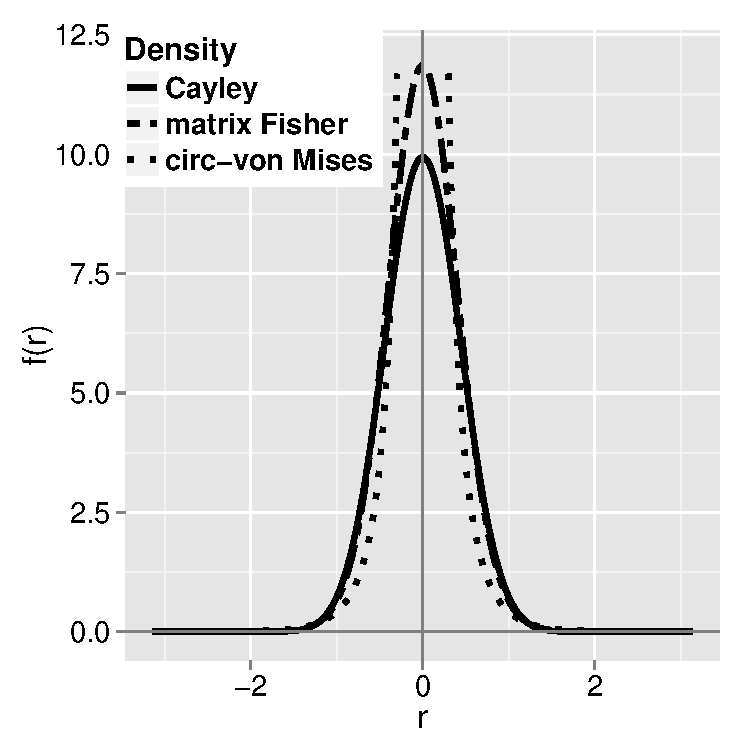
\includegraphics[width=0.33\textwidth]{Var25DensityHaar.pdf}}
% \subfloat[$\nu=0.50$]{\label{fig:fishden}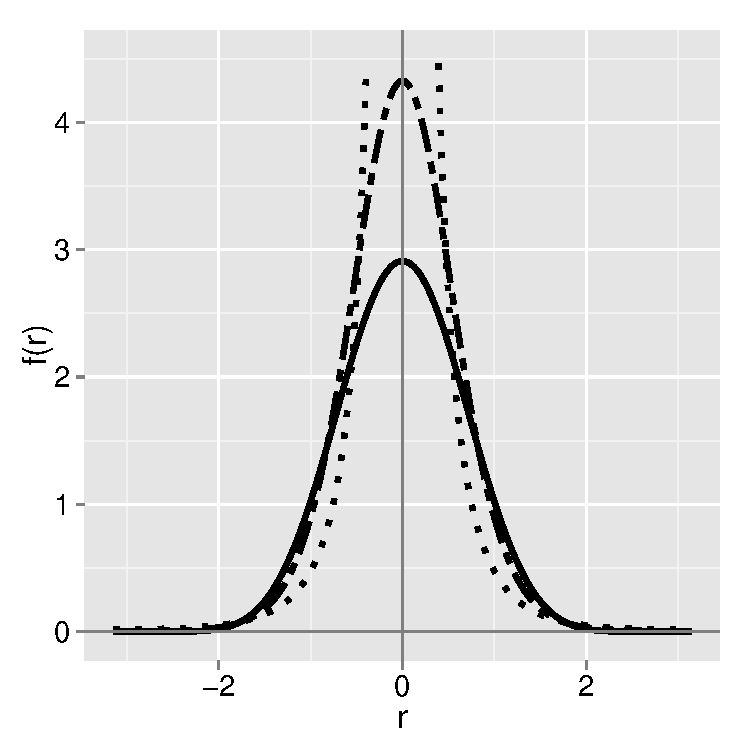
\includegraphics[width=0.33\textwidth]{Var5DensityHaar.pdf}}
% \subfloat[$\nu=0.75$]{\label{fig:vonmden}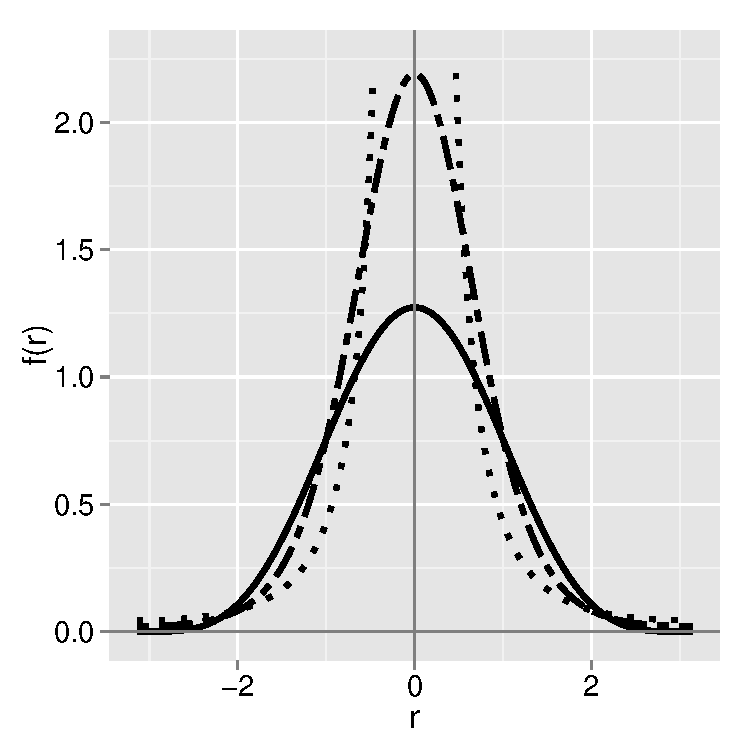
\includegraphics[width=0.33\textwidth]{Var75DensityHaar.pdf}}
% \caption{Density functions for the three rotational distributions with respect to the Haar measure. The solid line corresponds to the density of matrix Fisher distribution, the dashed line the density of the circular-von Mises-based distribution and the dotted line to the density of the Cayley distribution.}
% \label{fig:Haar}
% \end{figure}

\begin{figure}[h!]
\centering
\subfloat[Overview]{\label{fig:zoomout}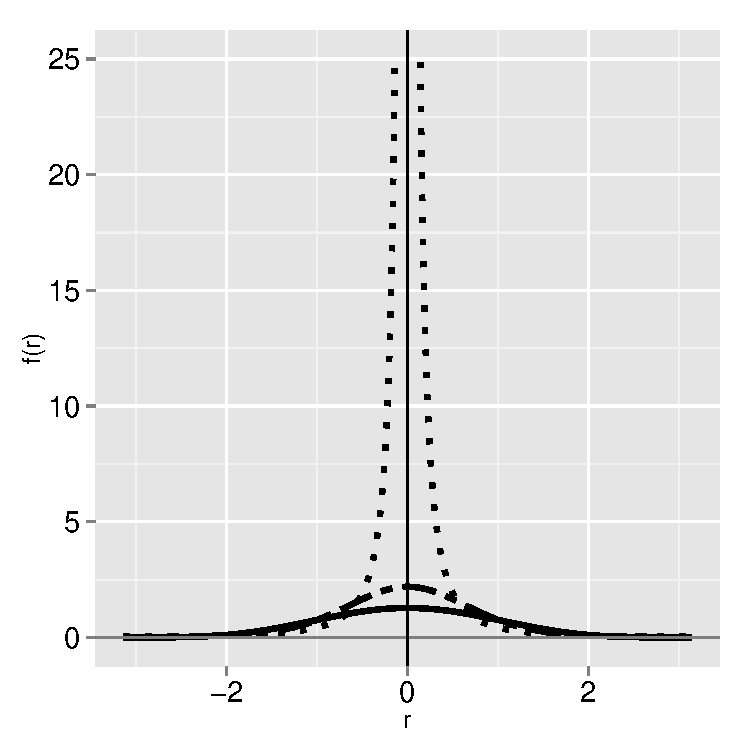
\includegraphics[width=0.33\textwidth]{Var75DensityHaarFullNoGuide.pdf}}
\subfloat[Mode Behavior]{\label{fig:body}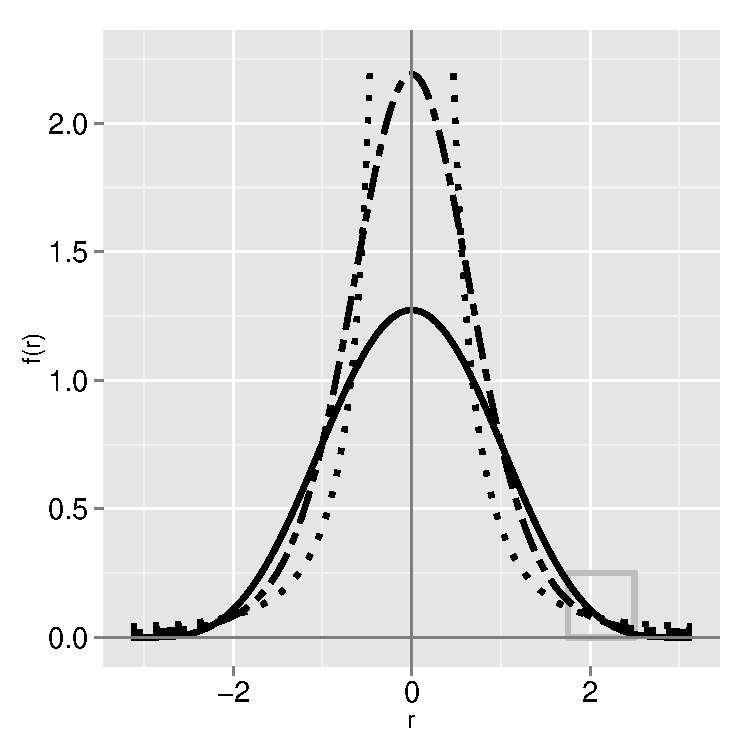
\includegraphics[width=0.33\textwidth]{Var75DensityBox.pdf}}
\subfloat[Tail Behavior]{\label{fig:denzoom}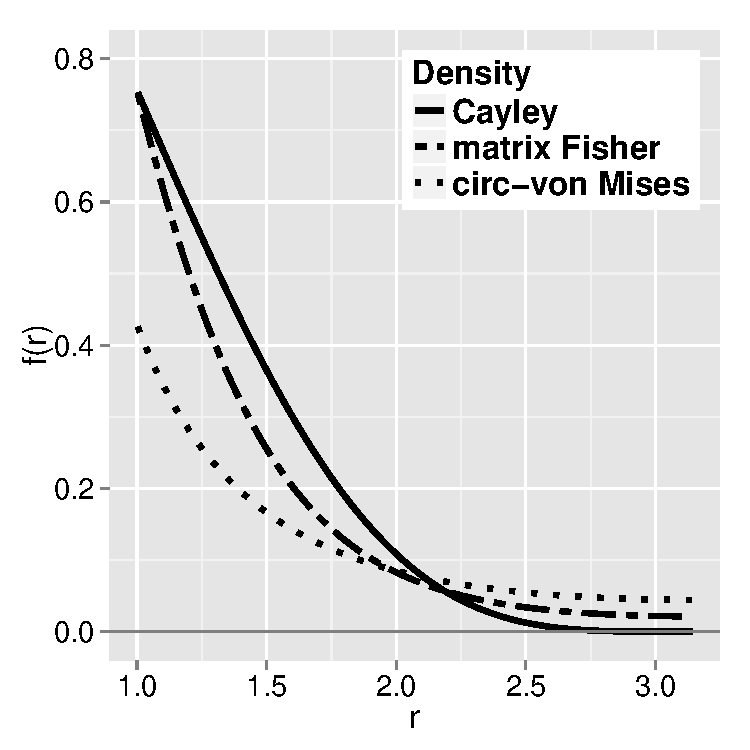
\includegraphics[width=0.33\textwidth]{Var75DensityZoom.pdf}}
\caption{Density comparison for rotation distributions with $\nu=0.75$.  The circular-von Mises based-distribution has the highest concentration, but also the heaviest tail.}
\label{fig:Haar}
\end{figure}

In Figures~\ref{fig:Haar}a and \ref{fig:Haar}b, we see that the circular-von Mises-based distribution has the most mass around the mode of zero whereas the Cayley distribution has the least mass around its mode.  Note that the circular variances for all three distributions are indeed the same, which would visually be more clear if the densities  were evaluated and plotted with respect to Lebesgue measure instead of the Haar measure. Figure~\ref{fig:Haar}c offers a better view of the tail behavior of the distributions.  The circular-von Mises-based distribution has the heaviest tail, while the Cayley distribution has the least mass in the tails. This will become important in the discussion of the results. A visualization of a random sample of 100 rotations, one sample for each of the three angular distributions, is given in the sphere plots in Figure~\ref{eyeballs}. The samples are adjusted to have a circular variance of $\nu = 0.25$.  Note that Figure~\ref{eyeballs} shows only the first of the three columns of each rotation matrix. We refer to the supplemental material online for a complete visualization of the three samples.
%Section~\ref{sec:appendix.eyeballs} 
\begin{figure}[htbp]
\centering
\subfloat[Cayley]{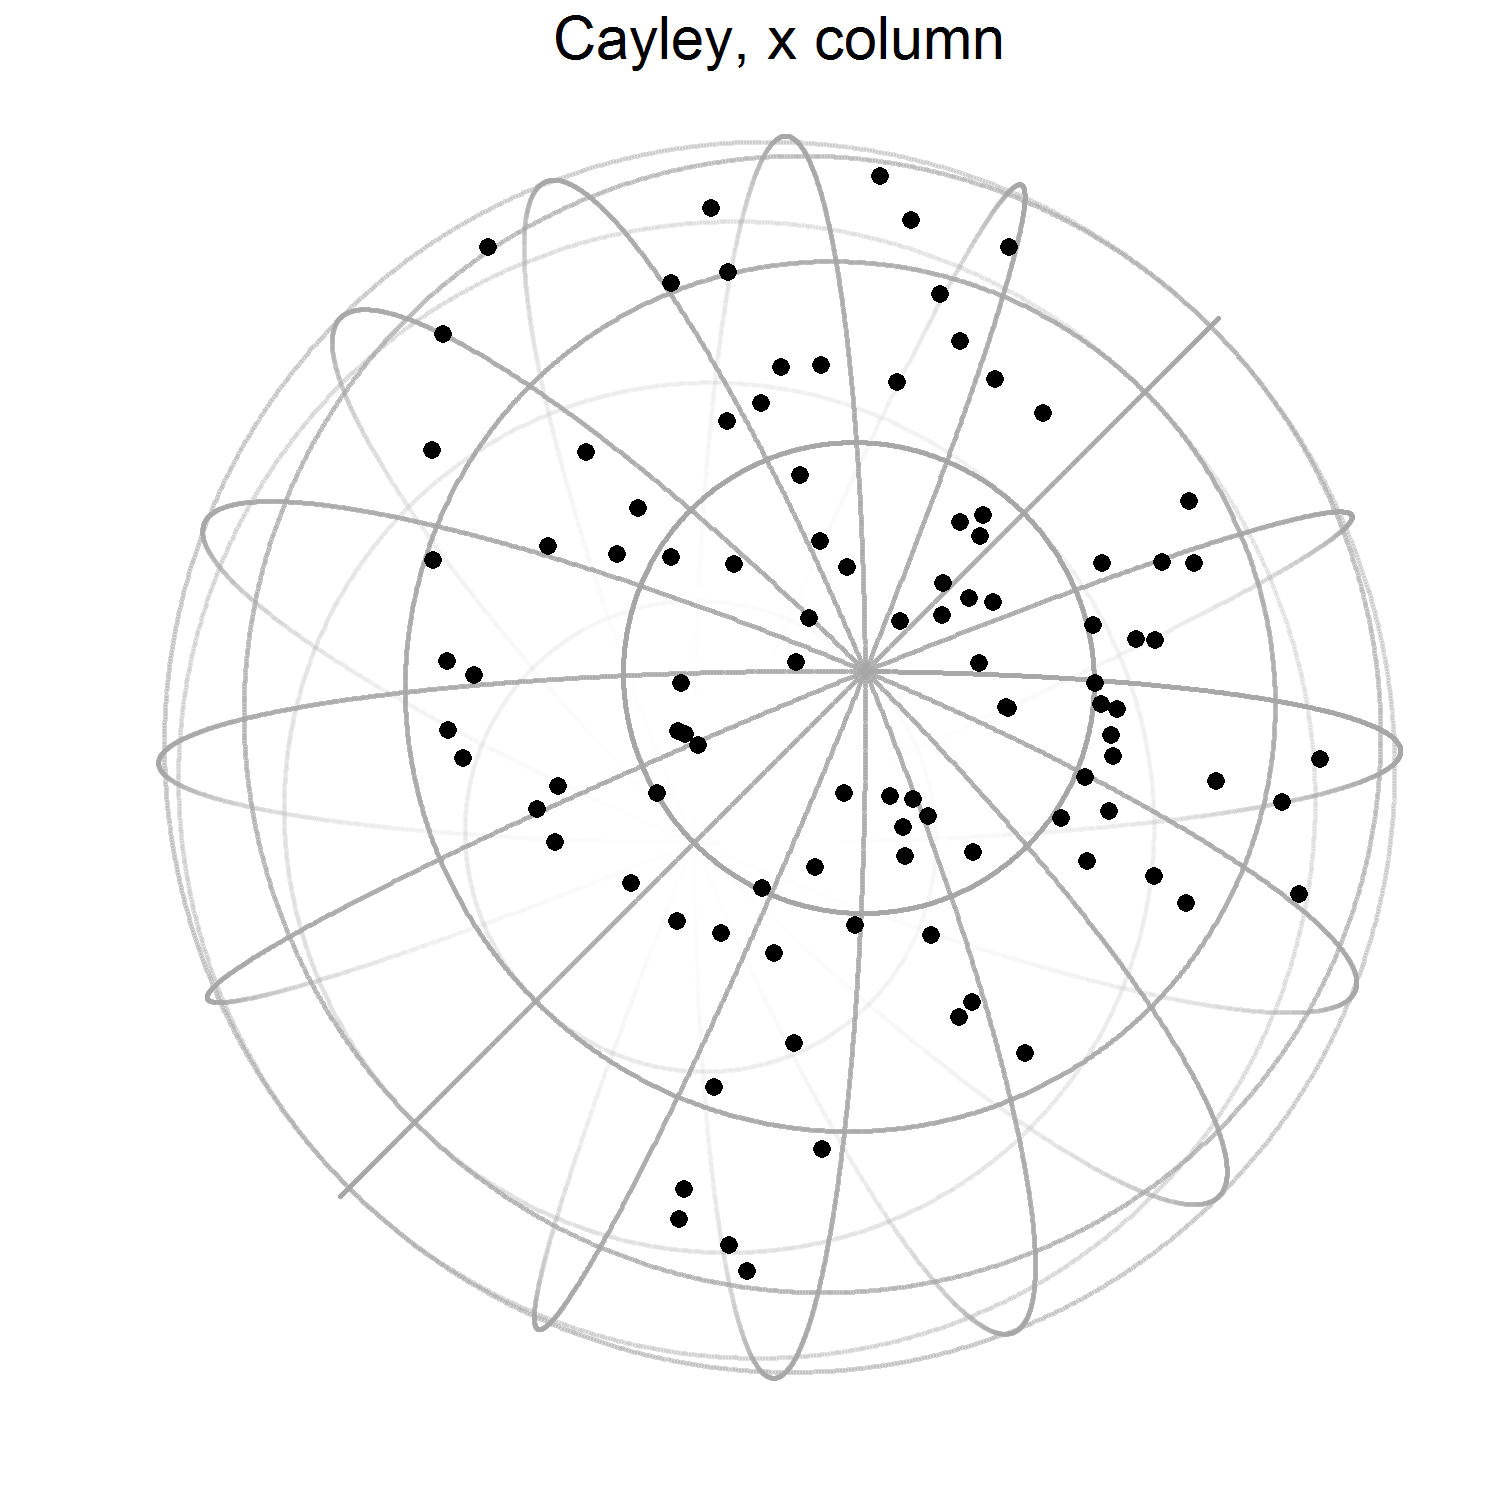
\includegraphics[width=.3\linewidth]{eye-cayley}}
\subfloat[matrix Fisher]{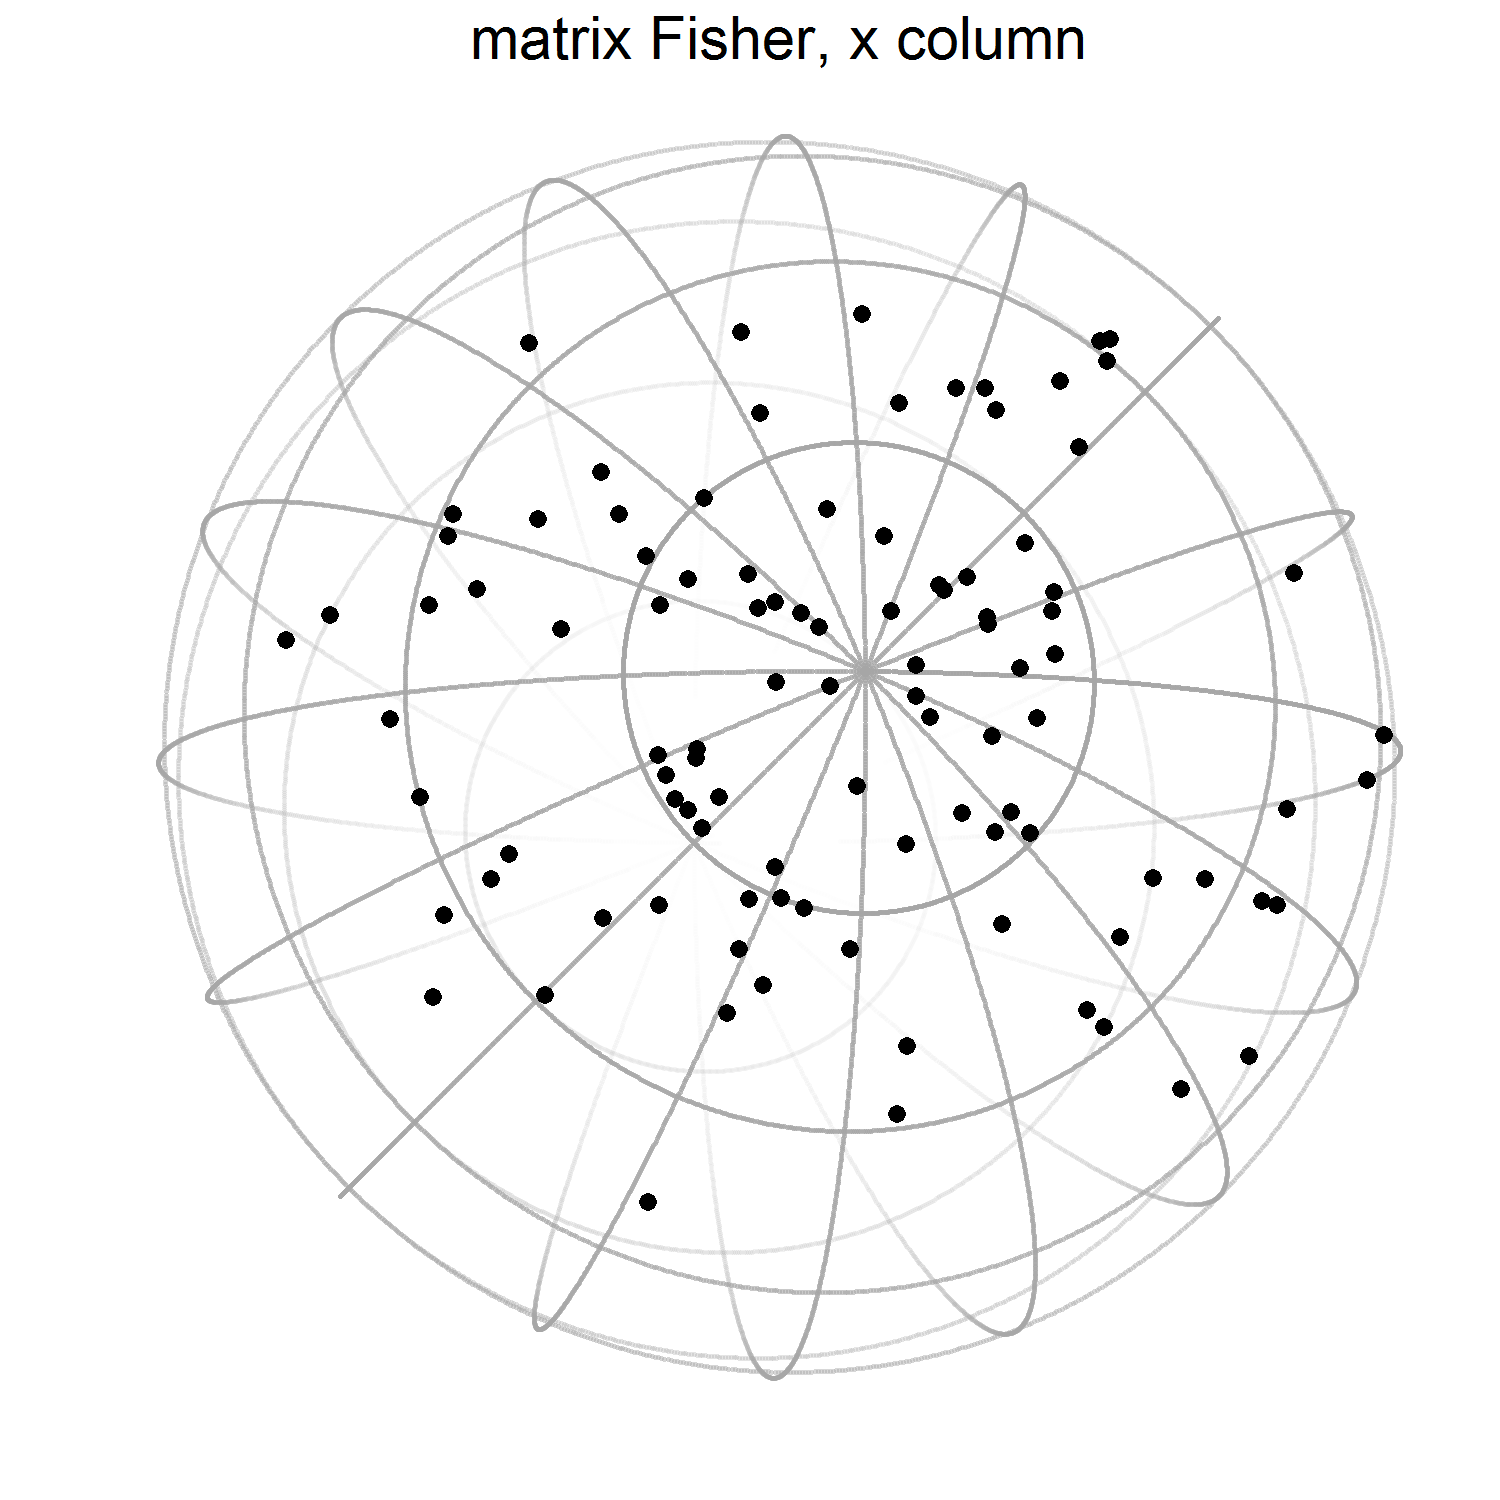
\includegraphics[width=.3\linewidth]{eye-fisher}}
\subfloat[circular-von Mises]{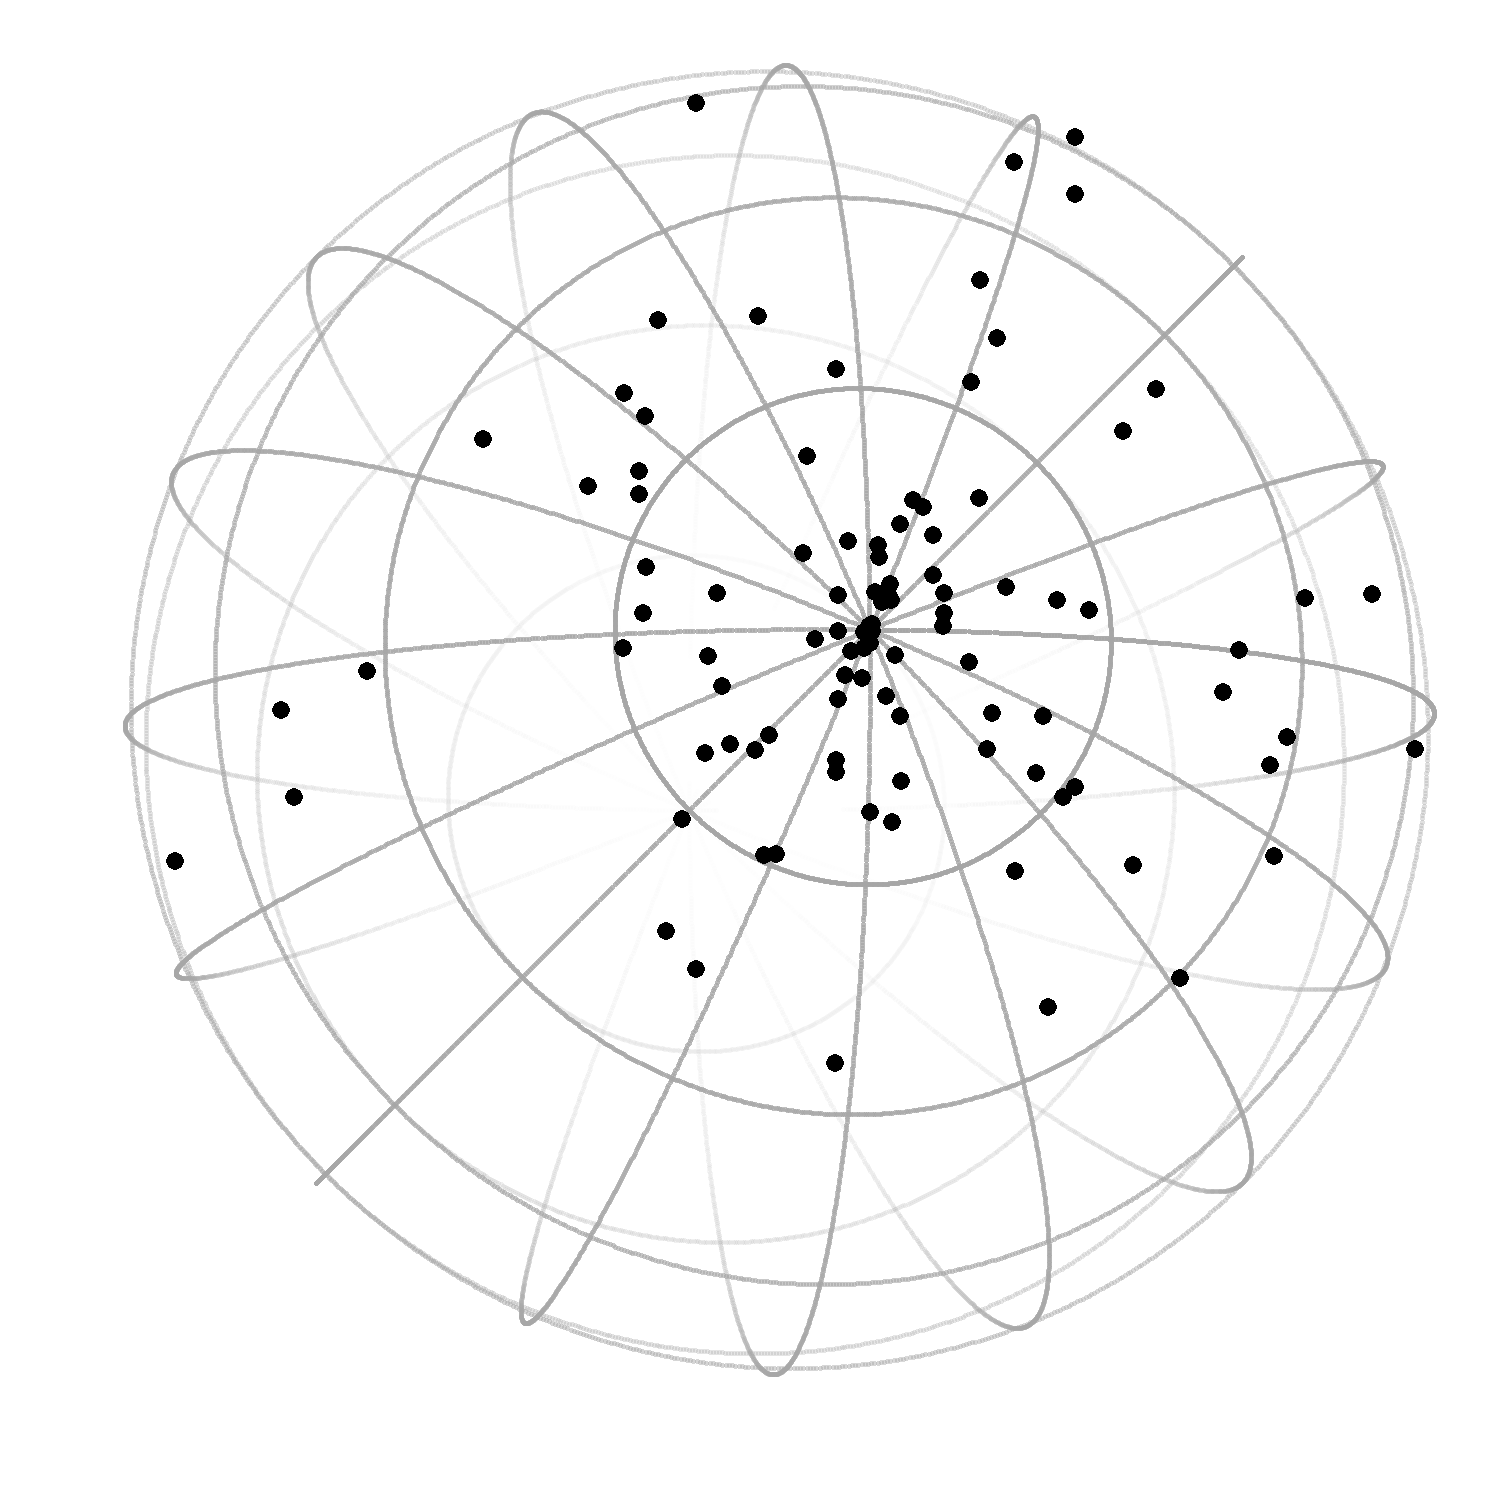
\includegraphics[width=.3\linewidth]{eye-vmises}}
\caption{\label{eyeballs}Sphere plots of the first column ($x$-axis) for randomly generated rotations with different distributions having  $\nu = 0.25$}
\end{figure}
In the simulation study to follow, for generating random rotation errors based on the construction above, we used different samplers to randomly generate angles $r\in(-\pi,\pi]$ from a given circular density, recalling that the form of $C(r|\kappa)$ depends on the intended symmetric distribution for the rotation errors $\bm{E}$, see also the supplemental material online.

%\subsection{Estimator Algorithms}
%\label{subsec:algorithms}

%Two of the estimators of interest require a projection from the space of all $3\times 3$ matrices, $\mathcal{M}(3)$, into $SO(3)$.  We perform this projection according to the following method.  For a matrix $\bm M\in\mathcal{M}(3)$ let $\lambda_1 \geq \lambda_2 \geq \lambda_3$ denote the ordered eigenvalues of $\bm M^\top\bm M$ with corresponding eigenvectors $ \bm u_1, \bm u_2, \bm u_3$.  Defining $\bm U=[\bm u_1, \bm u_2, \bm u_3]$ and provided that $\det(\bm M)\neq 0$, the unique projection of $\bm M$ into $SO(3)$ is given by
%\[
%\bm M\bm{U} \text{diag}\left(\frac{1}{\sqrt{\lambda_1}},\frac{1}{\sqrt{\lambda_2}},\frac{\text{sign}\left[\det(\bm M)\right]}{\sqrt{\lambda_3}}\right) \bm{U}^\top.
%\]
%We will refer to this as the $\mathcal{M}(3)$ projection algorithm. To calculate $\widehat{\bm{S}}_P$ given a sample $\{\bm{R}_1,\dots,\bm{R}_n\}\subset SO(3)$ we compute the $\mathcal{M}(3)$ projection of $\bar{\bm R}=\frac{1}{n}\sum_{i=1}^n\bm{R}_i$.  See \citet{arun87,horn88} and \citet{umeyama91} for an introduction and refinements of this solution including special cases such as $\det(\bar{\bm R})=0$.

%To compute the projected median $\widetilde{\bm S}_P$ we use a Weiszfeld-type algorithm originally given by \cite{weiszfeld37}.  The algorithm requires an initial value that does not equal any sample point. For the purpose of speeding up computing time we use $\widehat{\bm S}_P$ as the starting point. Note that the solution is generally not sensitive to the choice of starting points unless the data exhibit extreme spread.
%\begin{enumerate}
%\item Set $\widehat{\bm S}=\widehat{\bm S}_{P}$ and choose an arbitrarily small stopping rule $\varepsilon$.
%\item For $i=1,\ldots,n$ compute $\bm s_i=\bm R_i-\widehat{\bm S}$.
%\item Calculate
%\[
%\bar{\bm R}_W=\frac{\sum_{i=1}^n\bm R_i/||\bm s_i||_F}{\sum_{i=1}^n1/||\bm s_i||_F}
%\]
%which we call the weighted mean with respect to $\widehat{\bm S}$.
%\item Define $\widehat{\bm S}_{\text{new}}$ to be the $\mathcal{M}(3)$ projection of $\bar{\bm R}_W$.
%\item If $\varepsilon>||\widehat{\bm S}-\widehat{\bm S}_{\text{new}}||_F$ return $\widetilde{\bm{S}}_P=\widehat{\bm S}_{\text{new}}$; otherwise set $\widehat{\bm S}=\widehat{\bm S}_{\text{new}}$ and return to step 2.
%\end{enumerate}

%The second set of algorithms is based on the relationship between $SO(3)$ and its tangent space $\mathfrak{so}(3)$ through the principal logarithm of a rotation $\bm R$, see Sections~\ref{subsec:geometry} and \ref{subsec:metrics}. The rotation that minimizes the sum of the squared geodesic distances, $\widehat{\bm S}_G$, for a given tolerance level $\varepsilon$ can be found as follows \citep[see][]{manton04}.
%\begin{enumerate}
%\item Initiate a value for $\widehat{\bm S}$, e.g. $\widehat{\bm S}= \widehat{\bm S}_P$ .
%\item Calculate $\bm s=\frac{1}{n}\sum_{i=1}^n\Log(\widehat{\bm{S}}^\top\bm R_i)$.
%\item If $||\bm s||_F<\varepsilon$ return $\widehat{\bm S}_{G}=\widehat{\bm S}$; otherwise set $\widehat{\bm S}=\widehat{\bm S}\exp(\bm s)$ (see Section~\ref{subsec:geometry}), repeat step 2 and re-evaluate.
%\end{enumerate}


%Finally, to find the minimizer of the first order geodesic distances we use an algorithm developed by \citet{hartley11}.  Similar to $\widetilde{\bm S}_{P}$, this algorithm requires a starting point not in the sample, so we use $\widehat{\bm S}_{G}$ to save computational time.
%\begin{enumerate}
%\item Set $\widehat{\bm S}=\widehat{\bm S}_{G}$.
%\item For each sample point compute $\bm s_i=\Log(\widehat{\bm S}^\top\bm R_i)$.
%\item Set 
%\[
%\bm\delta=\frac{\sum_{i=1}^n \bm s_i/||\bm s_i||_F}{\sum_{i=1}^n 1/||\bm s_i||_F}.
%\]
%\item If $||\bm\delta||_F<\varepsilon$ then return $\widetilde{\bm S}_{G}=\widehat{\bm S}$; otherwise update $\widehat{\bm S}=\exp(\bm\delta)\widehat{\bm S}$ and return to step 2.
%\end{enumerate}


$\GeomMedian$ % !TEX root = Stanfill_CoDA.tex
\section{Results}\label{sec:results}

In this section we summarize and present the main findings of the simulation study for  estimating the central direction $\bm S = \bm I_{3\times 3}$ with the four proposed estimators of Section~\ref{sec:estimators}. We quantify the estimation error between the true location $\bm S = \bm I_{3\times 3}$ and an estimate $\widehat{\bm S}$ using the geodesic distance, i.e.  
\begin{equation}
\Rdist(\bm{S}, \widehat{\bm{S}}) =  \frac{1}{\sqrt{2}}||
\Log(\bm{S}^\top\widehat{\bm{S}})||_F, \quad \mbox{where} \quad \widehat{\bm{S}} =  \ProjMean, \; \GeomMean,\;  \ProjMedian \; \mbox{or} \; \GeomMedian.
\end{equation}

\noindent Note that for any two rotations $\bm R_1$ and $\bm R_2$ in $SO(3)$ it holds that their Euclidean distance $\Edist(\bm R_1,\bm R_2)=2\sqrt{2}\sin[\Rdist(\bm R_1,\bm R_2)/2]$ (see the supplemental material online for a short proof of this).  Hence, results using $\Edist$ would prove equivalent, albeit on a smaller scale.   
%\begin{center}
\begin{figure}[h!]
\centering
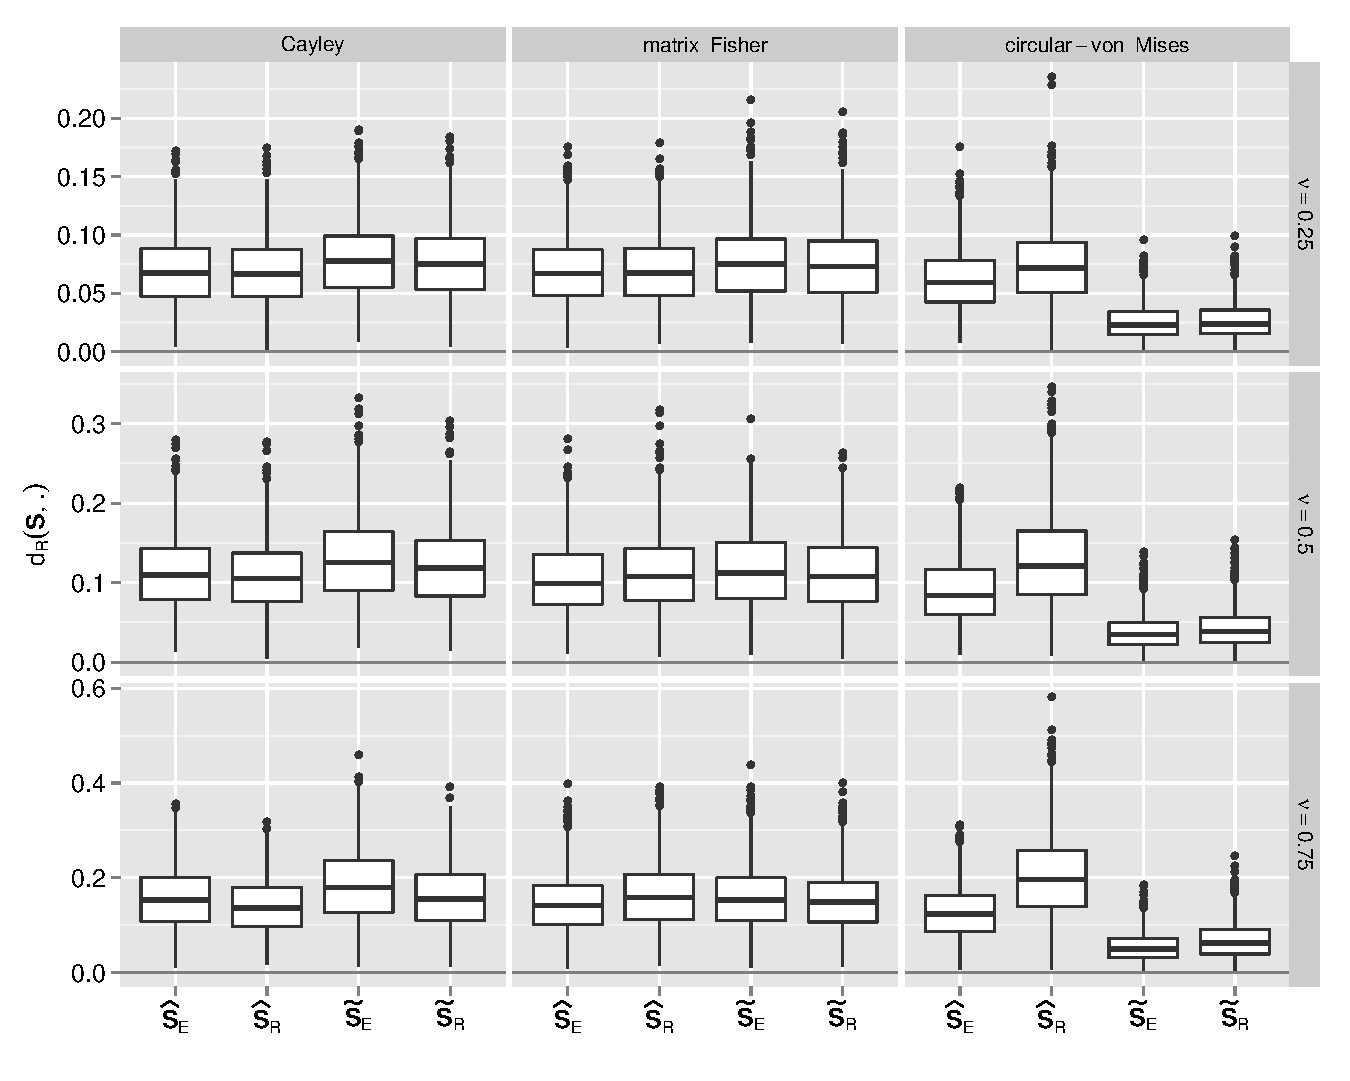
\includegraphics[width=0.8\textwidth]{N100AllNuBoxes.pdf}
\caption{Boxplots of the estimation errors for each rotation distribution and level of $\nu$,  $n=100$.}
\label{fig:NuBoxes}
\end{figure}
%\end{center}
Figure~\ref{fig:NuBoxes} displays side-by-side boxplots showing the estimation errors of all four estimators for a given choice of rotation distribution and circular spread $\nu$ when  $n=100$.   For a tabular summary of this figure including the root mean square error (RMSE)  as well as the \textit{mean estimation error} and estimated standard errors we refer to Table \ref{tab:alldN100} in Section~\ref{sec:appendix3} of the Appendix. 
First and foremost the results suggest that different location estimators emerge as preferable depending on the type of distribution assumed for the rotation errors in \eqref{eqn:1}.  For the circular-von Mises-based distribution both median-type estimators ($\ProjMedian$ and $\GeomMedian$) are superior with respect to the estimation error while for the Cayley and matrix Fisher models the mean-type estimators ($\ProjMean$ and $\GeomMean$) perform slightly better though on a less pronounced scale.   Figure~\ref{fig:NuBoxes} further shows that the estimation error is a function of the circular spread $\nu$; as $\nu$ decreases the range of the observed estimation errors decreases within each rotation model and for each of the four estimators. The same holds for the mean estimation error and RMSE.  Similarly, the estimation error decreases as the sample size $n$ increases. This result is shown in Figure~\ref{fig:NBoxes} in the supplemental material online.\\
While preferences within the median- and mean-type estimators are visible, these generally disappear as the variability in the data, i.e.~$\nu$ decreases.  For the Cayley and the matrix Fisher distribution the overall pattern of estimation is similar. $\ProjMean$ and $\GeomMean$ typically exhibit less spread and a lower average estimation error than $\ProjMedian$ and $\GeomMedian$ with differences between the estimators lessening as $\nu$ becomes smaller.\\
Figure~\ref{fig:vmnu75} illustrates the extent to which the mean estimation error and RMSE as a function of sample size differ with respect to estimator choice for the circular-von Mises-based distribution when $\nu=0.75$.  We can see more clearly the advantage of the median estimators over the mean estimators across sample sizes.
 \begin{figure}[h!]
\centering
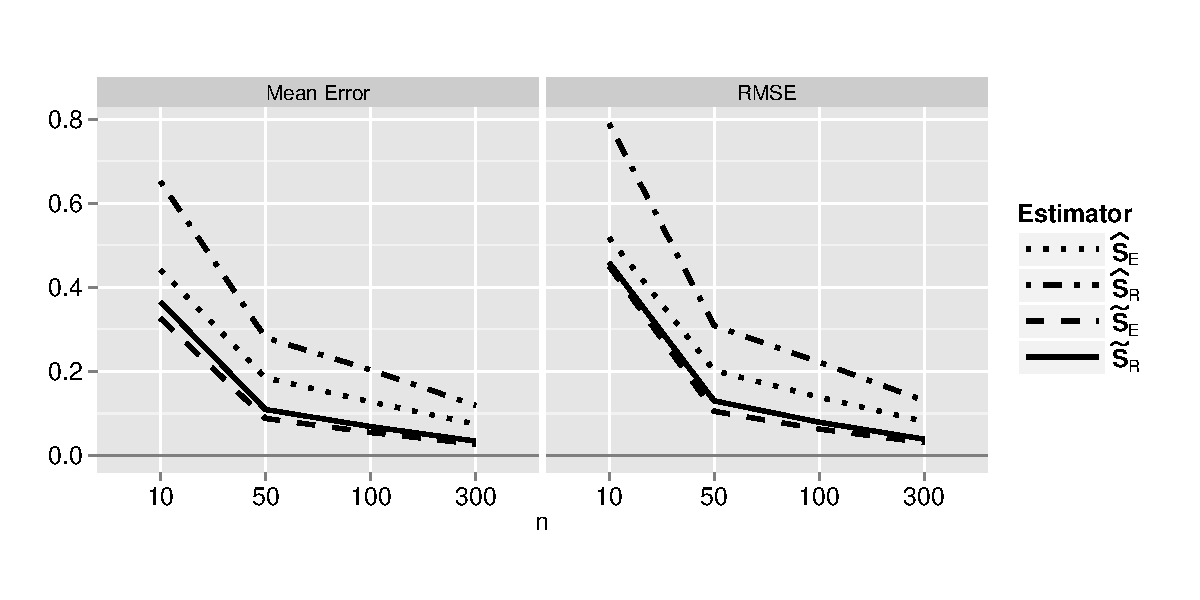
\includegraphics[width=0.8\linewidth]{vonMisesnu75MeanRMSE.pdf}
\caption{Plot of the estimation error for all levels of $n$ for the circular-von Mises-based distribution,  $\nu=0.75$.}  \label{fig:vmnu75}
\end{figure}
The previous findings raise the question why, unlike the Cayley and the Fisher matrix distribution, the circular-von Mises-based distribution so clearly distinguishes between the mean- and median-type estimators. A first insight can be obtained from Figures~\ref{fig:Haar} (b) and (c) which reveal that out of the three distributions the circular-von Mises-based distribution exhibits the heaviest tail. Thus, we can expect a larger proportion of   \textit{more extreme} observations to be sampled under the circular-von Mises-based distribution suggesting that a median-type estimator is more favorable. 
We use Figure \ref{fig:SimTail} to examine the extent to which the tail-behavior indeed accounts for the observed differences in the mean- and median-type estimators. Figure \ref{fig:SimTail} displays for each sample the proportion of observations in the sample considered to come from the tail of the distribution plotted against the difference in errors for the mean- and median-type estimators.  The results shown in Figure \ref{fig:SimTail} are with respect to the Euclidean geometry-based estimators $\ProjMean$ and $\ProjMedian$. Similar results are obtained for the Riemannian geometry-based estimators $\GeomMean$ and $\GeomMedian$ and therefore are omitted. Note that we define the tail to be the average crossing point at which the distributions cross for the second time, see Figure~\ref{fig:denzoom}. From  Figure \ref{fig:SimTail} we can see that with an increase in the proportion of tail observations the error of the mean estimator indeed increases at a higher rate than does the error of the median estimator, i.e.~the relative difference in the errors plotted on the $y$-axis increases. As a result the projected median is preferable to the projected mean more often as the tail becomes heavier.  \\
\begin{figure}[h!]
\centering
\vspace{-0.5cm}
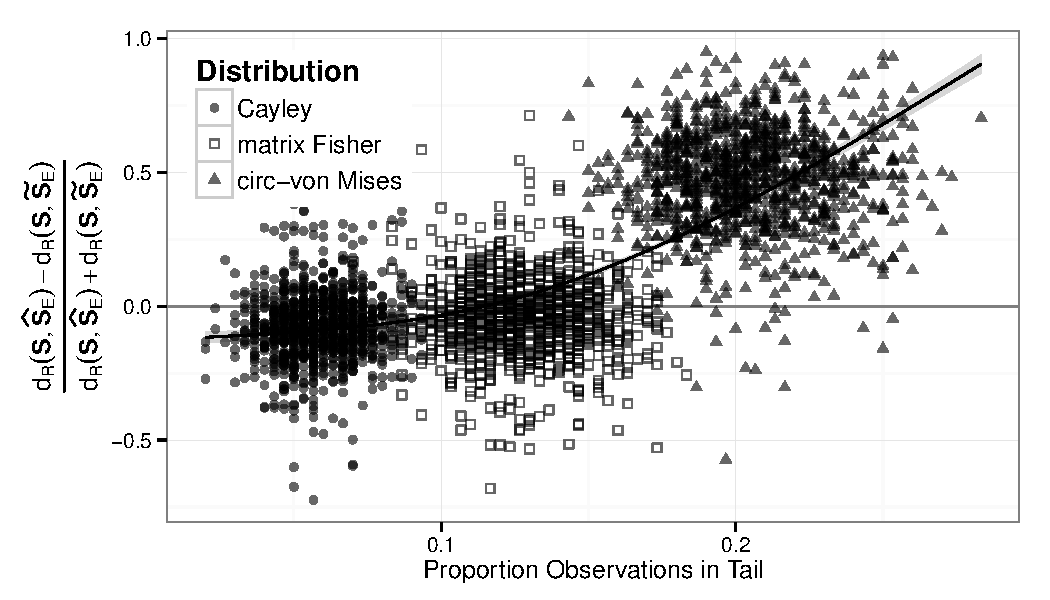
\includegraphics[width=.8\textwidth]{Nu75N300TailBehaviorStandard}
\caption{The proportion of observations in the tail against the difference in projected mean and median errors for simulated data with $n=300$.  Different symbols indicate different error distributions.}
\label{fig:SimTail}
\end{figure}

\noindent We next explore how the choice of geometric distance (Euclidean $\Edist$ or Riemannian $\Rdist$) \red{affects} the estimation error for both types of loss functions (i.e., $L_2-$norm or $L_1-$norm yielding a mean- or median type estimator, respectively). To provide more insight into the observed differences we plot in Figure~\ref{fig:comPL2} on the $x$-axis for each type of loss function  the estimation errors resulting from using $\Edist$ versus the corresponding estimation errors resulting from using $\Rdist$ ($y$-axis) for $n=100$ and $\nu=.25$,  $\nu=.75$, respectively.   Estimators based on the $L_2-$norm  are represented by black dots whereas the $L_1-$norm based estimators correspond to light gray dots. For example, Figure \ref{fig:comPL2} suggests that  $\GeomMedian$ tends to yield less estimation error than $\ProjMedian$  for the Cayley distribution as most of the points fall below the identity line while the Riemannian distance-based estimators $\GeomMedian$ and $\GeomMean$ result in greater errors for ${\bm S}$ than their Euclidean distance based counterparts for the circular-von Mises-based distribution. These findings support similar results for $\ProjMedian$ and $\GeomMedian$ seen earlier in Figure~\ref{fig:NuBoxes}.
\begin{figure}[h!]
\centering
\subfloat{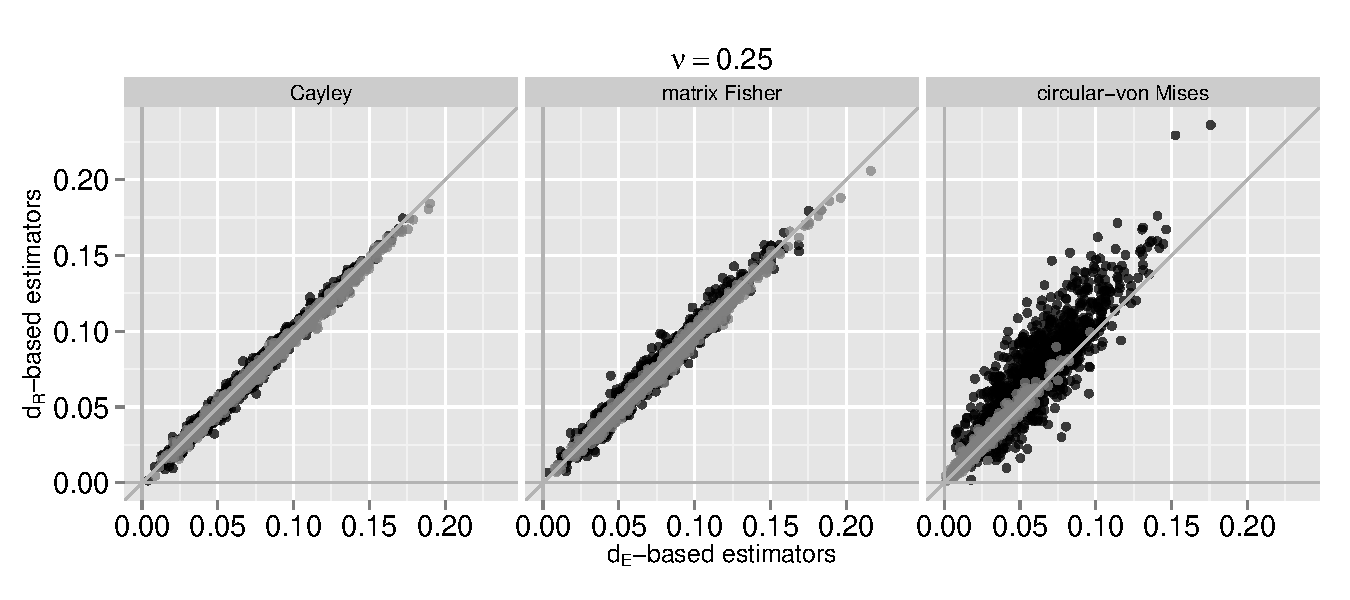
\includegraphics[width=0.8\linewidth]{EuclidRiemannNu25.pdf}}\\
\subfloat{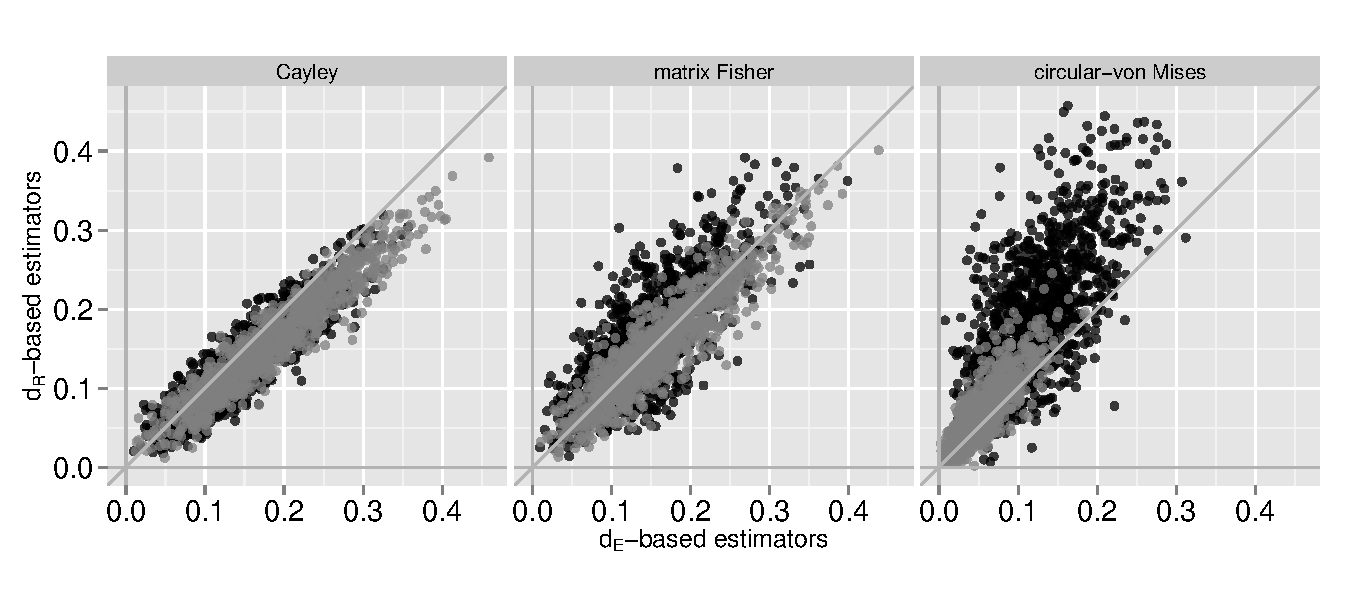
\includegraphics[width=0.8\linewidth]{EuclidRiemannNu75.pdf}}
\caption{Comparison of the estimation errors resulting from $\Edist$ ($x$-axis) and $\Rdist$ ($y$-axis) approaches, $n=100$.  The $L_2-$norm based estimators are in black dots and the $L_1-$norm based estimators are in light gray.}
\label{fig:comPL2}
\end{figure}
Tables \ref{tab:percL1} and \ref{tab:percL2} of the supplemental material online support Figure~\ref{fig:comPL2} with an exact count (expressed as a percentage) of how often $\Rdist$ resulted in a smaller estimation error than $\Edist$.  Additionally, we show the average amount of error by which the Riemannian $\Rdist-$ and Euclidean $\Edist-$based estimates deviate from one another.   
Earlier results suggested the use of median-type estimators for the circular-von Mises-based distribution. Taking the findings with respect to the choice of geometry into account, we consider $\ProjMedian$ preferable for the circular-von Mises-based distribution as $\Rdist(\ProjMedian,\bm S) < \Rdist(\GeomMedian,\bm S)$ most of the time.  For the Cayley distribution our preference regarding the geometry is reversed; although differences are subtle $\Rdist$ is the preferred metric for the Cayley distribution especially when $\nu$ is large and overall $\GeomMean$ typically exhibits the least spread for this distribution as perhaps best illustrated in Table~\ref{tab:alldN100}.   For the  matrix Fisher distribution the preference is less clear, especially for less variable data, but as $\nu$ increases the Euclidean-based mean yields generally a smaller estimation error more often. In summary,
\begin{itemize}
\item the choice of location estimator can depend on the rotation error distribution in the location model (1).  For the matrix Fisher and the Cayley distribution  the projected arithmetic mean $\ProjMean$ and the geometric mean $\GeomMean$ are, respectively, preferable though $\ProjMedian$ and $\GeomMedian$ are not far behind especially when the circular spread is smaller. For the circular-von Mises-based distribution  the projected median $\ProjMedian$  should be used.

\item   a significant finding of the simulation results is that the (Euclidean-based)  projected median $\ProjMedian$ is typically a good location estimator across rotation error models.  For the circular-von Mises-based estimation, this generally has the best performance, while for the Cayley or matrix Fisher distributions, this estimator is often quite comparable to the best estimator.  In other words, $\ProjMedian$, an estimator  not previously considered for rotation matrices in the literature, appears to be suggestible, particularly in small samples and without knowledge of the underlying rotation error distribution.

\end{itemize}
% !TEX root = Stanfill_CoDA.tex
\section{Data Application}\label{sec:data}

We consider electron backscatter diffraction (EBSD) data obtained by scanning a fixed  12.5 $\mu$m $\times$ 10 $\mu$m nickel surface at individual locations spaced 0.2 $\mu$m apart. This scan was repeated 14 times for each location yielding a total of 3,449 observations, \citep{bingham09, bingham10b}. Every observation corresponds to the orientation, expressed as a rotation matrix, of a cubic crystal on the metal surface at a particular location. One goal of processing ESBD data is to identify the main orientation of cubic crystals in the metal, where graphs of cubic crystals with similar orientations constitute ``grains'' on the metal surface, thus making the estimation of the main direction $\bm S$ for a sample of rotations relevant here.

At every location, using the 14 repeat scans  we computed the misorientation angle $|r|=\Rdist(\widehat{\bm{S}}, \bm I_{3\times 3})$ of the four estimators ($\widehat{\bm{S}}= \ProjMean$, $\ProjMedian$, $\GeomMean$, and $\GeomMedian$) to compare resulting differences in the corresponding estimates.  In the following we will focus particularly on the differences between $\ProjMean$ and $\ProjMedian$ as the Riemannian estimators  $\GeomMedian$ and $\GeomMean$ largely agree with their Euclidean counterparts. 

Figure~\ref{fig:grain-map}a illustrates the implementation of $\ProjMedian$: each location on the plot is colored according to the mis-orientation angle between  the estimate $\ProjMedian$  and the identity $\bm I_{3\times 3}$ (as an arbitrarily chosen reference point).  The plot shows a distinct spatial structure resembling a grain map. In Figure~\ref{fig:grain-map}b we illustrate the difference between $\ProjMean$ and $\ProjMedian$ at each location. The difference in estimates is again defined with respect to the mis-orientation angle between both estimates and locations are colored accordingly. 
%
\begin{figure}[h!] %  figure placement: here, top, bottom, or page
   \centering
%   \vspace{-.45in}
   \subfloat[{Shading reflects angle between  $\ProjMedian$ and $\bm I_{3\times 3}$}]{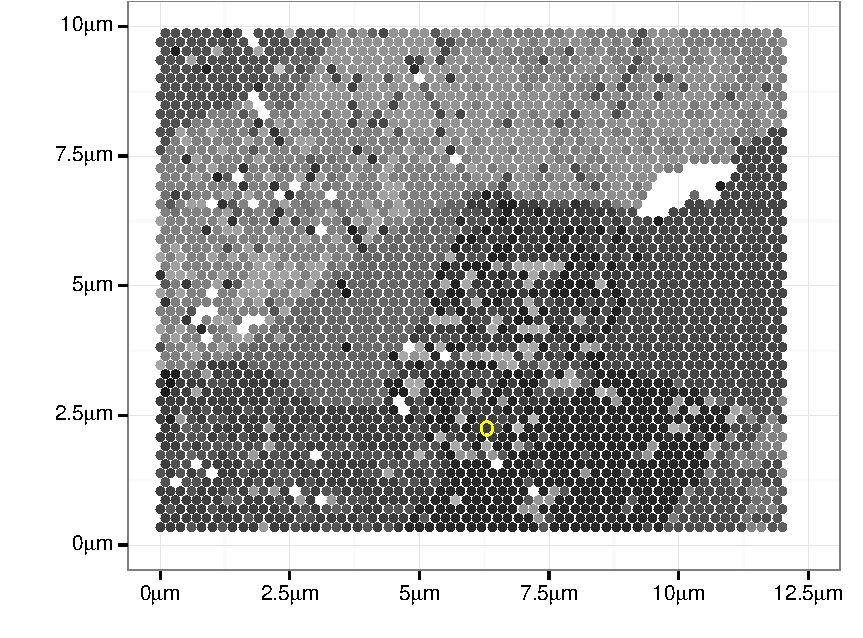
\includegraphics[width=.4\textwidth]{images/grain-map-wo.pdf}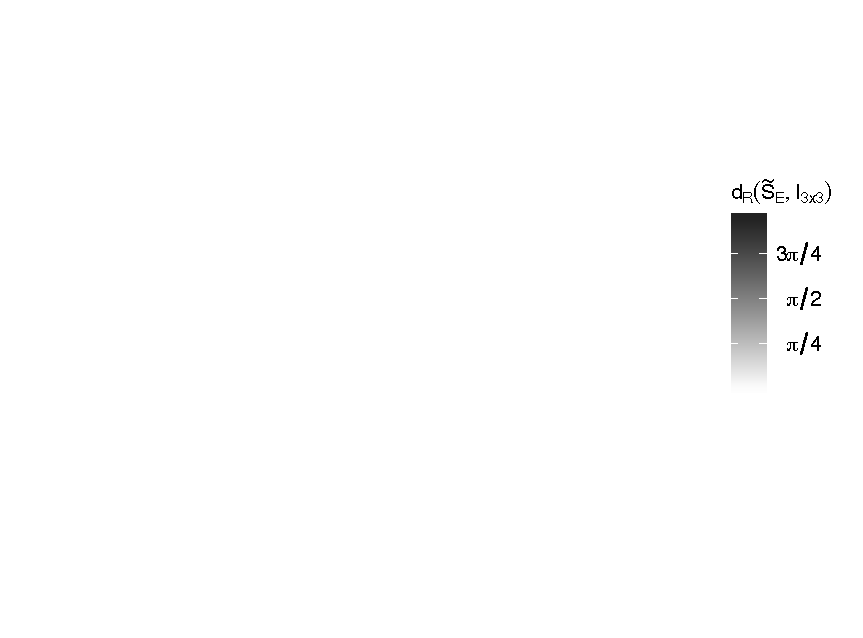
\includegraphics[width=.06\textwidth]{images/grain-map-legend.pdf}} \hfill
   \subfloat[{Location shaded by angle (in degrees) between  $\ProjMedian$ and $\ProjMean$. Distances of 0.5$^\circ$ or more are generally considered to suggest different main orientations. Note that the mapping of distance to color shading is on a square-root scale.}]{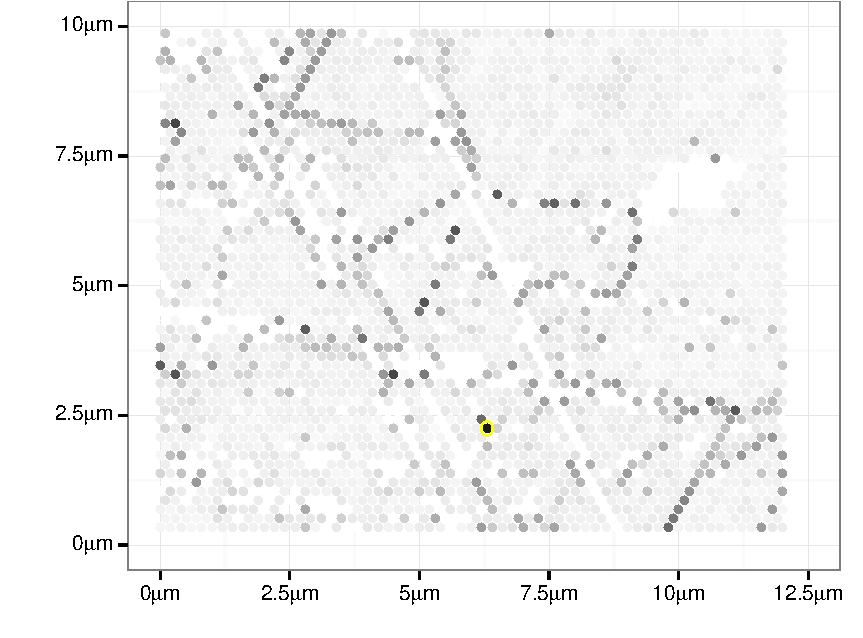
\includegraphics[width=.4\textwidth]{images/grain-diff-wo.pdf}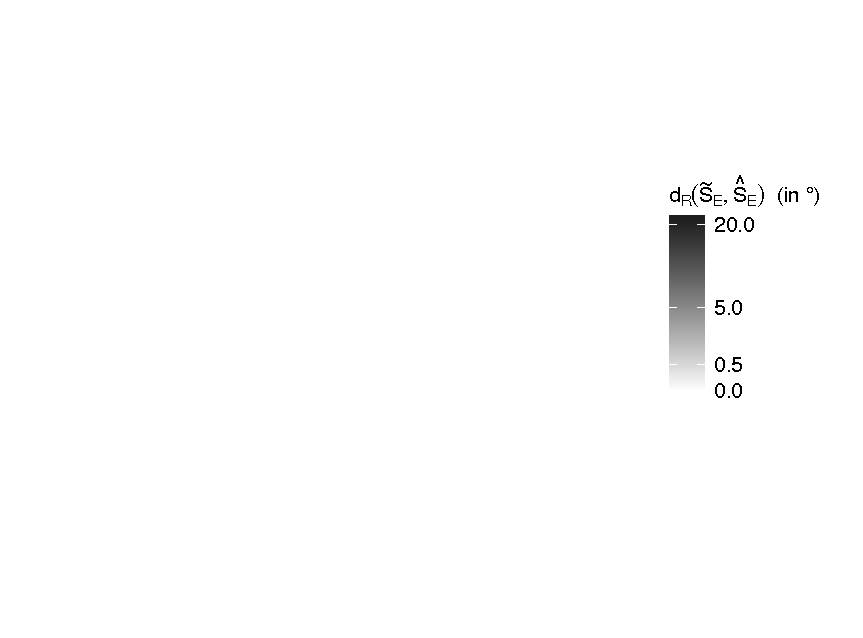
\includegraphics[width=.08\textwidth]{images/grain-diff-legend.pdf}}
%    \vspace{-.175in} 
   \caption{ \label{fig:grain-map}  Display of all locations of the investigated nickel surface. Each dot corresponds to one location and shading reflects  angles. The location of the the largest difference between estimators $\ProjMedian$ and $\ProjMean$ is circled.}
\end{figure}
%
Note that the literature, e.g. \cite{bingham10b}, suggests that distances of $0.5^\circ$ degrees are indicative of different grains. In our example, about 10\% of the locations result in a difference between $\ProjMean$ and $\ProjMedian$ estimates of at least that size. Differences tend to be largest along boundaries between the spatial structures in Figure~\ref{fig:grain-map}b  (i.e.~identifying boundaries). This results a different allocation of a location to different grains depending on the choice of estimation method.

As an example, Table~\ref{tab:rotations} contains the observed orientations (the collection of all nine coefficients $x_{ij}$, $1 \le i,j \le 3$, of the $3\times 3$ rotation matrix) for each of the 14 repeated scans at the location with the largest observed difference between $\ProjMedian$ and $\ProjMean$, namely 22.3$^\circ$ (circled in Figure~\ref{fig:grain-map}). 
 
%Table~\ref{tab:rotations} provides an explanation for the observed differences between $\ProjMedian$ and $\ProjMean$ along the spatial structure in Figure~\ref{fig:grain-map}. 

The scans have been re-ordered to better illustrate  the clustering of the rotations observed at this particular location. 
   The clusters suggest that, for this location on a ``grain boundary,'' a subset of the scans likely picked up the orientation of a neighboring cubic crystal  belonging to a different grain. A median-type estimator naturally does better for such data with ``outliers'' than a mean-type estimator.  
\begin{table}[h!]
\caption{\label{tab:rotations} List of all rotations in the location with the largest difference between mean and median estimators. We observe one main cluster and one smaller cluster with three additional rotations in the proximity. }
\begin{center}
\scalebox{0.75}{
\begin{tabular}{crrrrrrrrrr}
  \hline
scan& & $x_{11}$ & $x_{12}$& $x_{13}$& $x_{21}$& $x_{22}$& $x_{23}$& $x_{31}$& $x_{32}$& $x_{33}$ \\ 
  \hline
1 & &  -0.646 & -0.552 & -0.527 & 0.464 & -0.833 & 0.303 & -0.606 & -0.049 & 0.794 \\ 
2 & & -0.641 & -0.550 & -0.535 & 0.459 & -0.834 & 0.307 & -0.615 & -0.048 & 0.787 \\ 
3 & & -0.640 & -0.549 & -0.537 & 0.457 & -0.834 & 0.309 & -0.618 & -0.048 & 0.785 \\ 
4 & &  -0.639 & -0.546 & -0.542 & 0.462 & -0.836 & 0.297 & -0.615 & -0.061 & 0.787 \\ 
5 & & -0.639 & -0.547 & -0.540 & 0.456 & -0.835 & 0.307 & -0.619 & -0.050 & 0.783 \\ 
6 & & -0.638 & -0.550 & -0.540 & 0.459 & -0.834 & 0.307 & -0.619 & -0.052 & 0.784 \\ 
7 & & -0.637 & -0.551 & -0.540 & 0.459 & -0.833 & 0.309 & -0.620 & -0.051 & 0.783 \\ 
8 & & -0.633 & -0.554 & -0.540 & 0.464 & -0.830 & 0.309 & -0.619 & -0.055 & 0.783 \\ [5pt]
9 & & -0.068 & -0.422 & -0.904 & 0.994 & -0.105 & 0.025 & -0.084 & -0.900 & 0.427 \\ [5pt]
10 & & -0.017 & -0.633 & -0.774 & 0.961 & -0.224 & 0.162 & -0.276 & -0.741 & 0.612 \\ [5pt]
11 & & -0.005 & -0.551 & -0.834 & 0.982 & -0.158 & 0.099 & -0.186 & -0.819 & 0.542 \\ 
12 & & -0.002 & -0.587 & -0.809 & 0.978 & -0.167 & 0.124 & -0.208 & -0.792 & 0.574 \\ 
13 & & -0.002 & -0.595 & -0.804 & 0.974 & -0.182 & 0.132 & -0.225 & -0.783 & 0.580 \\ [5pt]
14 & & -0.727 & -0.475 & -0.496 & 0.138 & -0.809 & 0.572 & -0.672 & -0.348 & 0.653 \\ 
   \hline
\end{tabular}}
\vspace{-0.5cm}
\end{center}
\end{table}

We visualize Table~\ref{tab:rotations} and the estimates resulting from applying $\ProjMedian$ and $\ProjMean$ at this location in Figure \ref{fig:pcp} using a parallel coordinate plot: for every scan each of the nine coefficients $x_{ij}$ ($1 \le i,j \le 3$)) is plotted separately. Coefficients that correspond to the same scan are connected by a line.   Note that the coefficient values are jittered using a small perturbation in form of a rotation matrix to avoid over-plotting and to illustrate cluster sizes. The light- and dark green colored line represent the $\ProjMedian$ and $\ProjMean$ estimates of the main direction based on the 14 scans.   This example  illustrates that the median estimator, $\ProjMedian$,  can more reliably estimate the main direction in the presence of potential anomalies on the spatial boundaries of grains, as this estimate is located within the largest cluster of rotations, while the projected mean pulled into a location between the clusters.


%\begin{figure}[htbp] %  figure placement: here, top, bottom, or page
%   \centering
%   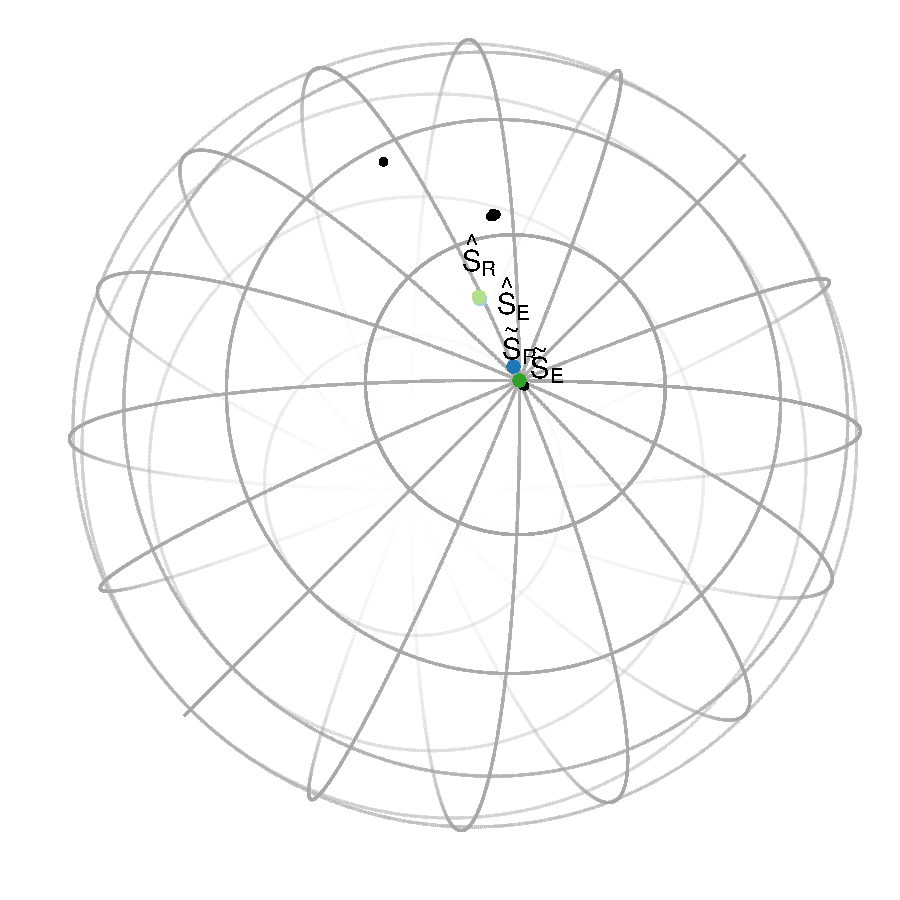
\includegraphics[width=.275\textwidth]{images/eyeball-1031-1.pdf} 
%   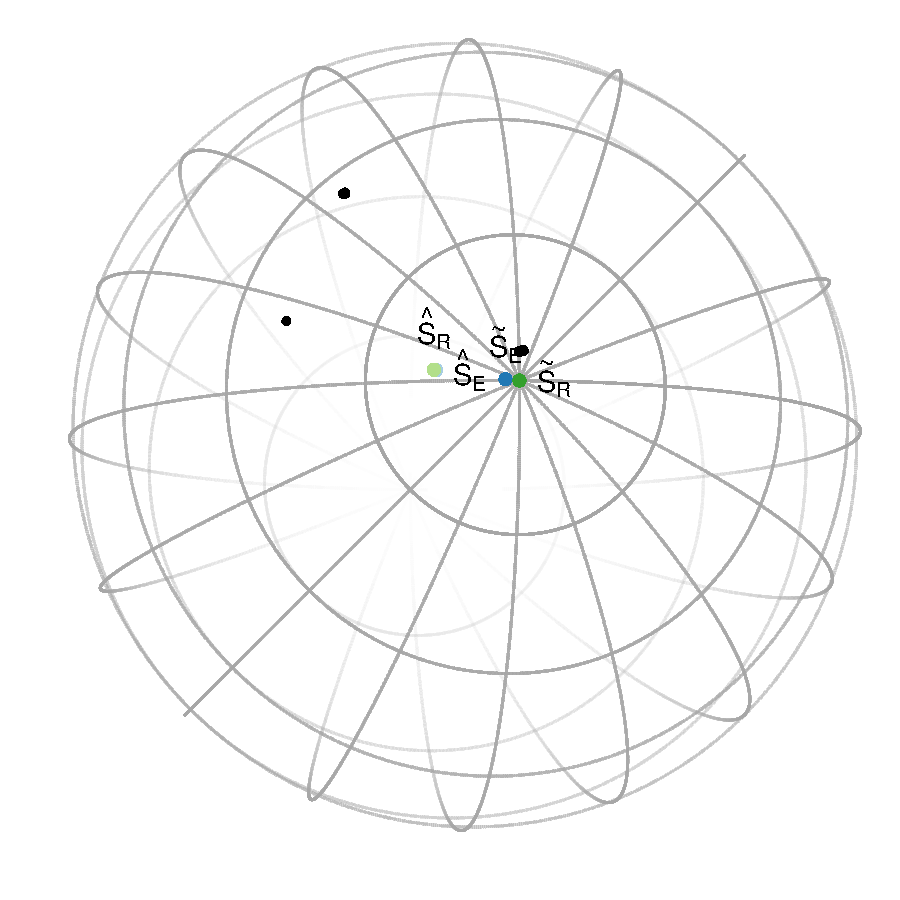
\includegraphics[width=.275\textwidth]{images/eyeball-1031-2.pdf} 
%   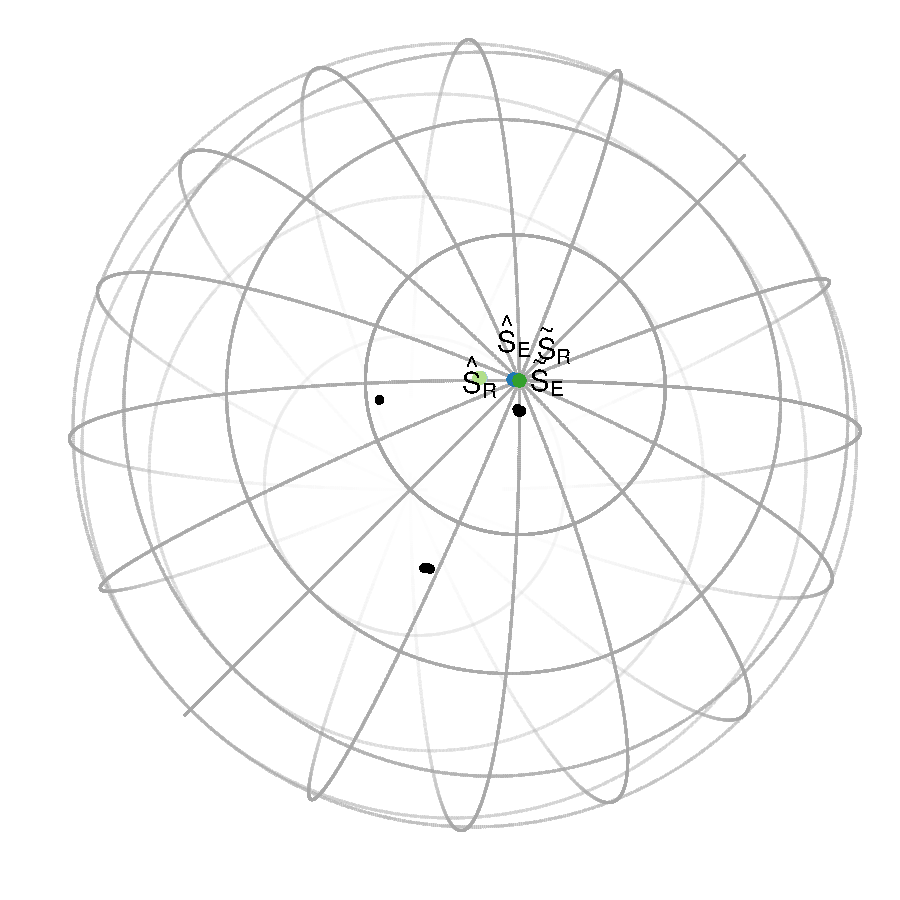
\includegraphics[width=.275\textwidth]{images/eyeball-1031-3.pdf} 
%   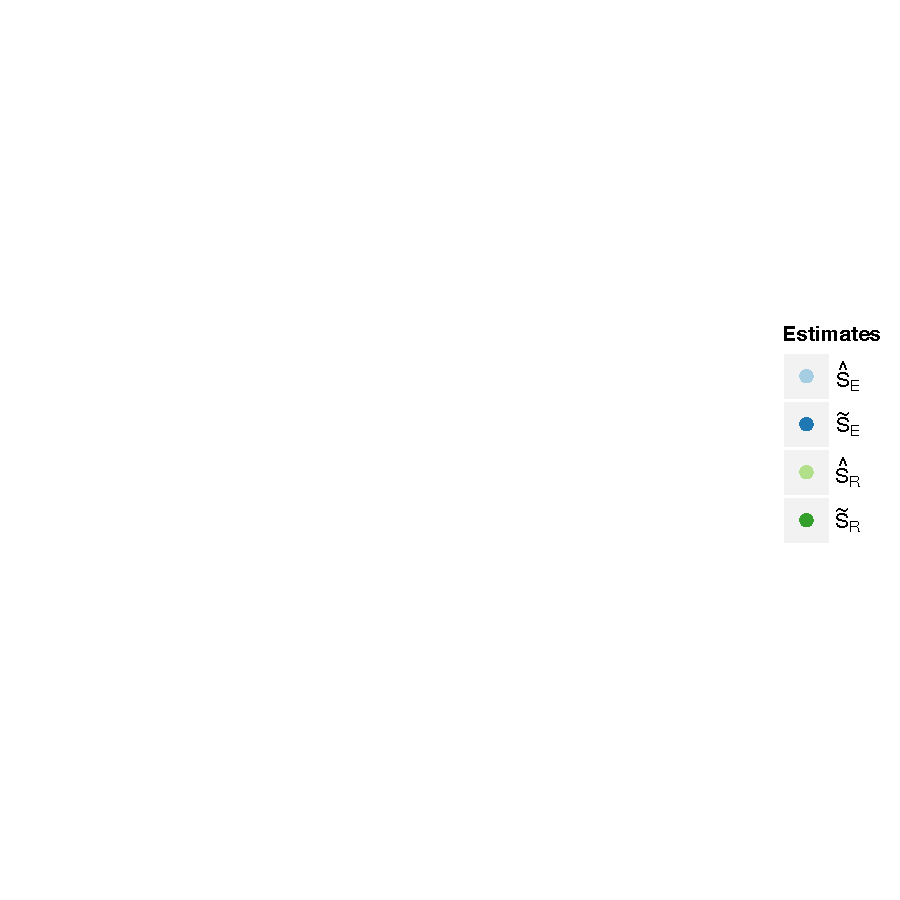
\includegraphics[height=.275\textwidth]{images/legend.pdf} 
%   \caption{ \label{fig:eyeballs-1}Sphere plots of EBSD measurements at a single location. The data sample is shown as dark grey points, the estimates of the main direction are colored and labelled. The clustering of the results makes the existence  of several main directions  quite obvious. }
%\end{figure}

\begin{figure}[htbp] %  figure placement: here, top, bottom, or page
   \centering
   \subfloat[Parallel coordinate plot. ]{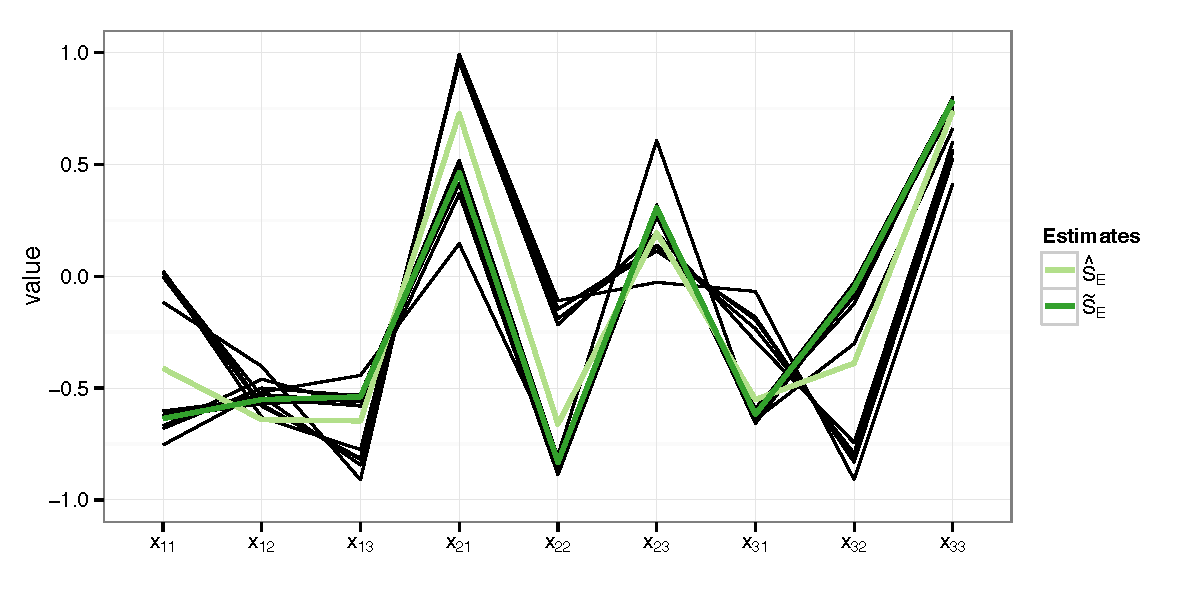
\includegraphics[height=.325\textwidth]{images/pcp.pdf}}
   \subfloat[Sphere plot of $y$-axis. ]{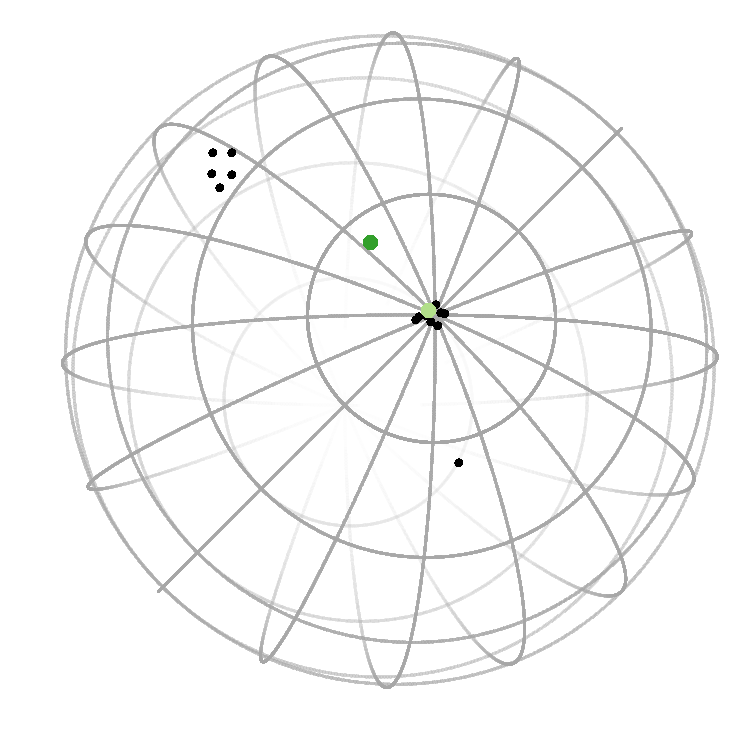
\includegraphics[height=.325\textwidth]{images/eye-698-2.pdf}}
   
   \caption{ \label{fig:pcp} Two views of all fourteen rotation matrices of table \ref{tab:rotations}, the location with the largest angle difference between projected mean and median estimator.}
\end{figure}

%=======
%% !TEX root = Stanfill_CoDA.tex
%\section{Data Application}\label{sec:data}
%
%We consider electron backscatter diffraction (EBSD) data obtained by scanning a fixed  12.5 $\mu$m $\times$ 10 $\mu$m nickel surface at individual locations spaced 0.2 $\mu$m apart. This scan was repeated 14 times for each location yielding a total of 3,449 observations, \citep{bingham09, bingham10b}. Every observation corresponds to the orientation, expressed as a rotation matrix, of a cubic crystal in the metal at a particular location. One goal of analyzing ESBD data is to identify the main orientation of cubic crystals in the metal, thus making the estimation of the main direction $\bm S$ for a sample of rotations important to the field.\\
%
%At every location we implemented each of the four estimators ($\ProjMean$, $\ProjMedian$, $\GeomMean$, and $\GeomMedian$) to compare resulting differences in the corresponding estimates.  In the following we will focus particularly on the differences between $\ProjMean$ and $\ProjMedian$ as the Riemannian estimators  $\GeomMedian$ and $\GeomMean$ largely agree with their Euclidean counterparts. 
%
%The left hand side of Figure~\ref{fig:grain-map} illustrates the implementation of $\ProjMedian$: each location on the plot is colored according to the mis-orientation angle between $\ProjMedian$  and the identity $\bm I_{3\times 3}$ (as an arbitrarily chosen reference point).  The plot shows a distinct spatial structure \blue{resembling a grain map}. On the right hand side of Figure~\ref{fig:grain-map} we illustrate the difference between $\ProjMean$ and $\ProjMedian$ at each location. The difference in estimates is again defined with respect to the mis-orientation angle between both estimates and locations are colored accordingly. Note that the literature, e.g. \cite{bingham10b}, suggests that distances of $0.5^\circ$ degrees are indicative of different grains. In our example, about 10\% of the locations result in a difference between $\ProjMean$ and $\ProjMedian$ estimates of at least that size. Differences tend to be largest along boundaries between the spatial structures on the left of Figure~\ref{fig:grain-map}.  
%\begin{figure}[htbp] %  figure placement: here, top, bottom, or page
%   \centering
%   \vspace{-.15in}
%   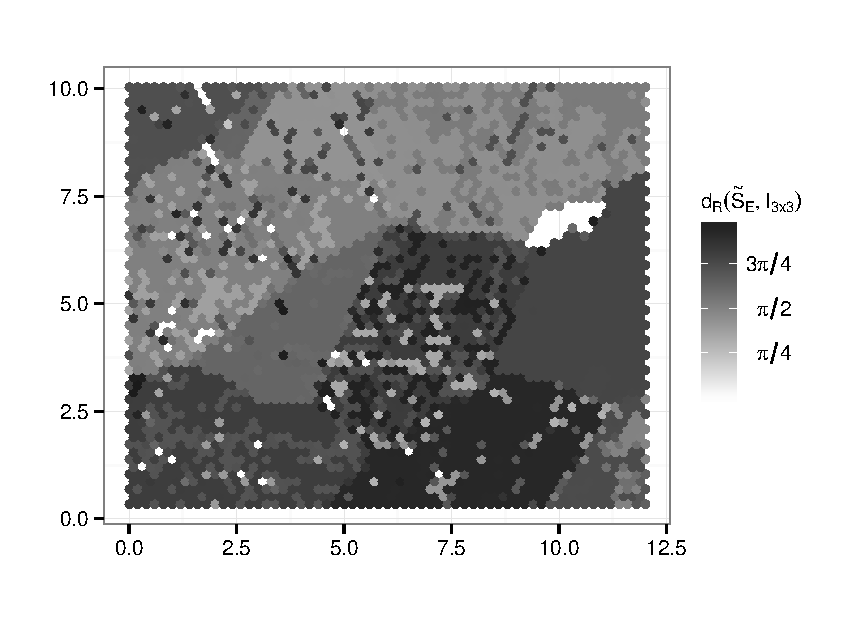
\includegraphics[width=.49\textwidth]{images/grain-map.pdf} 
%   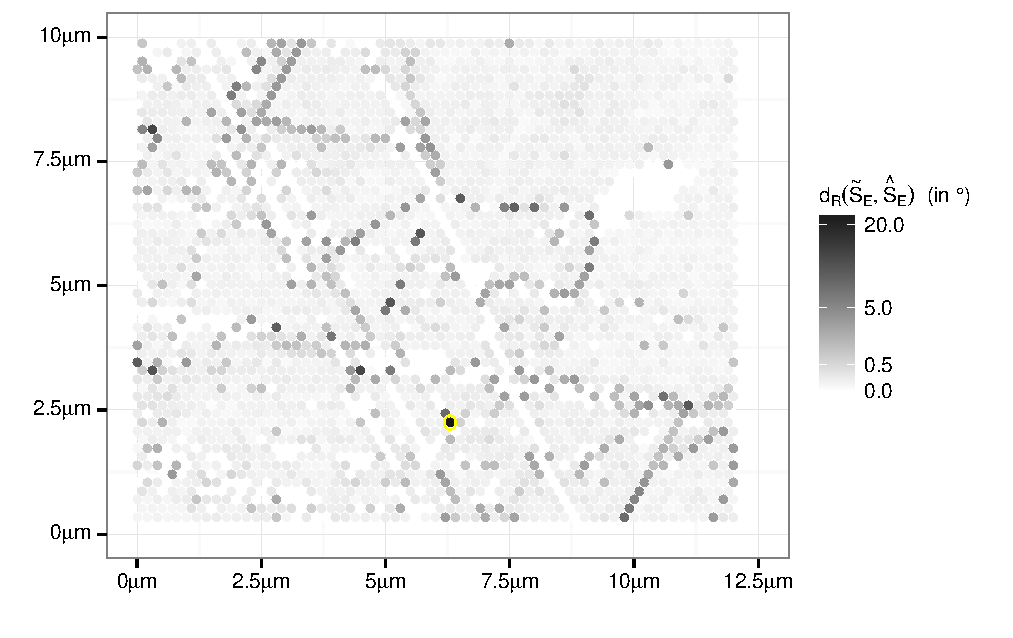
\includegraphics[width=.49\textwidth]{images/grain-diff.pdf} 
%    \vspace{-.175in} 
%   \caption{ \label{fig:grain-map}  Display of all locations of the investigated nickel surface (left). Each dot corresponds to one location, where shading reflects the angle between $\ProjMedian$ and $\bm I_{3\times 3}$. On the right, differences (in degrees) between $\ProjMedian$ and $\ProjMean$ estimates for each location are shown. Distances of 0.5$^\circ$ or more are generally considered to suggest different main orientations. Note that the mapping of distance to color shading is on a square-root scale.}
%\end{figure}
%Table~\ref{tab:rotations} provides an explanation for the observed differences between $\ProjMedian$ and $\ProjMean$ along the spatial structure in Figure~\ref{fig:grain-map}. The table contains the observed orientation (collection of all nine coefficients $x_{ij}$, $1 \le i,j \le 3$, of the $3\times 3$ rotation matrix) for each of the 14 repeated scans at the location with the largest observed difference between $\ProjMedian$ and $\ProjMean$, namely 22.3$^\circ$.   The scans have been re-ordered to better illustrate  three clusters of orientations observed at this particular location. The clusters suggest that for a subset of the scans the orientation from a neighboring cubic crystal, likely belonging to a different grain, was picked up instead of the orientation of the   target cubic crystal. A median-type estimator naturally does better for such data than a mean-type estimator.  
%\begin{table}[h!]
%\caption{\label{tab:rotations} List of all rotations in the location with the largest difference between mean and median estimators. We observe one main cluster and one smaller cluster with three additional rotations in the proximity. }
%\begin{center}
%\scalebox{0.75}{
%\begin{tabular}{crrrrrrrrrr}
%  \hline
%scan& & $x_{11}$ & $x_{12}$& $x_{13}$& $x_{21}$& $x_{22}$& $x_{23}$& $x_{31}$& $x_{32}$& $x_{33}$ \\ 
%  \hline
%1 & &  -0.646 & -0.552 & -0.527 & 0.464 & -0.833 & 0.303 & -0.606 & -0.049 & 0.794 \\ 
%2 & & -0.641 & -0.550 & -0.535 & 0.459 & -0.834 & 0.307 & -0.615 & -0.048 & 0.787 \\ 
%3 & & -0.640 & -0.549 & -0.537 & 0.457 & -0.834 & 0.309 & -0.618 & -0.048 & 0.785 \\ 
%4 & &  -0.639 & -0.546 & -0.542 & 0.462 & -0.836 & 0.297 & -0.615 & -0.061 & 0.787 \\ 
%5 & & -0.639 & -0.547 & -0.540 & 0.456 & -0.835 & 0.307 & -0.619 & -0.050 & 0.783 \\ 
%6 & & -0.638 & -0.550 & -0.540 & 0.459 & -0.834 & 0.307 & -0.619 & -0.052 & 0.784 \\ 
%7 & & -0.637 & -0.551 & -0.540 & 0.459 & -0.833 & 0.309 & -0.620 & -0.051 & 0.783 \\ 
%8 & & -0.633 & -0.554 & -0.540 & 0.464 & -0.830 & 0.309 & -0.619 & -0.055 & 0.783 \\ [5pt]
%9 & & -0.068 & -0.422 & -0.904 & 0.994 & -0.105 & 0.025 & -0.084 & -0.900 & 0.427 \\ [5pt]
%10 & & -0.017 & -0.633 & -0.774 & 0.961 & -0.224 & 0.162 & -0.276 & -0.741 & 0.612 \\ [5pt]
%11 & & -0.005 & -0.551 & -0.834 & 0.982 & -0.158 & 0.099 & -0.186 & -0.819 & 0.542 \\ 
%12 & & -0.002 & -0.587 & -0.809 & 0.978 & -0.167 & 0.124 & -0.208 & -0.792 & 0.574 \\ 
%13 & & -0.002 & -0.595 & -0.804 & 0.974 & -0.182 & 0.132 & -0.225 & -0.783 & 0.580 \\ [5pt]
%14 & & -0.727 & -0.475 & -0.496 & 0.138 & -0.809 & 0.572 & -0.672 & -0.348 & 0.653 \\ 
%   \hline
%\end{tabular}}
%\vspace{-0.5cm}
%\end{center}
%\end{table}
%
%  
%We visualize Table~\ref{tab:rotations} and the estimates resulting from applying $\ProjMedian$ and $\ProjMean$ at this location in Figure \ref{fig:pcp} using a parallel coordinate plot: for every scan each of the nine coefficients $x_{ij}$ ($1 \le i,j \le 3$)) is plotted separately. Coefficients that correspond to the same scan are connected by a line.   Note that the coefficient values are jittered using a small perturbation in form of a rotation matrix to avoid over-plotting and to illustrate cluster sizes. The light- and dark blue colored line represent the $\ProjMedian$ and $\ProjMean$ estimates of the main direction based on the 14 scans.   
%%Note that the figure shows a sample of a single location, yet the clustering in the data suggests clearly the presence of \emph{several} main directions. The same holds true for locations in the vicinity which happen to coincide with grain boundaries. 
%
%This example  illustrates that the median estimate, $\ProjMedian$,  can more reliably estimate the main direction in the presence of \red{clustered data}.
%
%
%%\begin{figure}[htbp] %  figure placement: here, top, bottom, or page
%%   \centering
%%   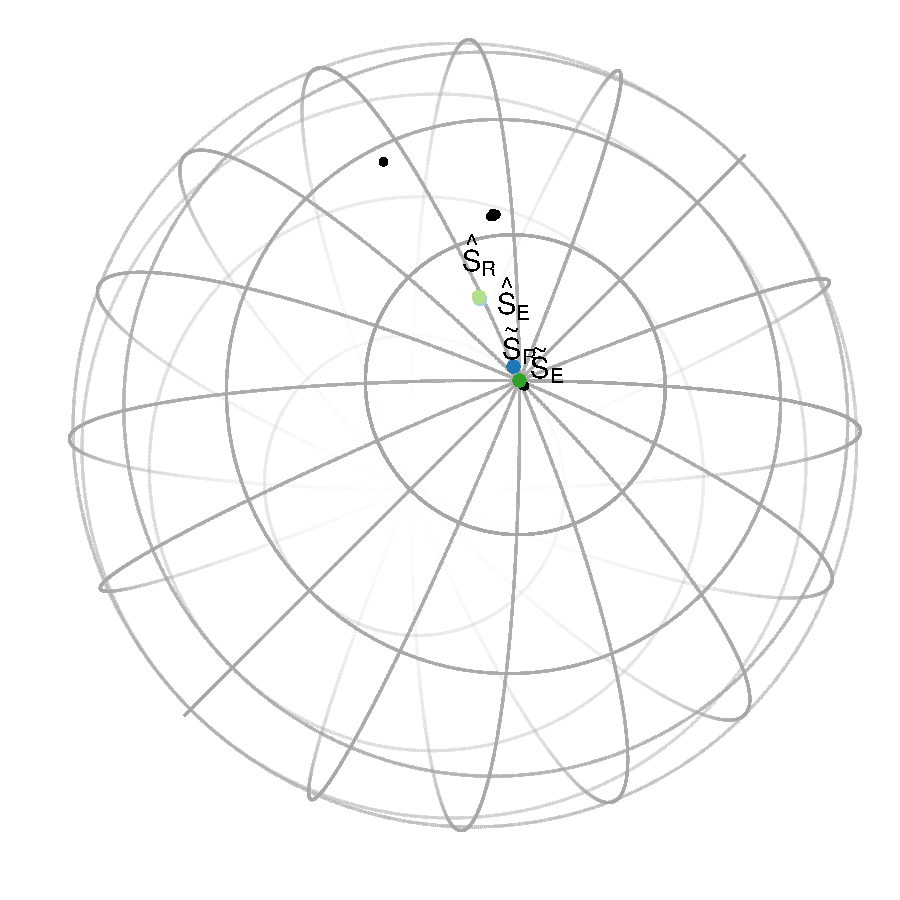
\includegraphics[width=.275\textwidth]{images/eyeball-1031-1.pdf} 
%%   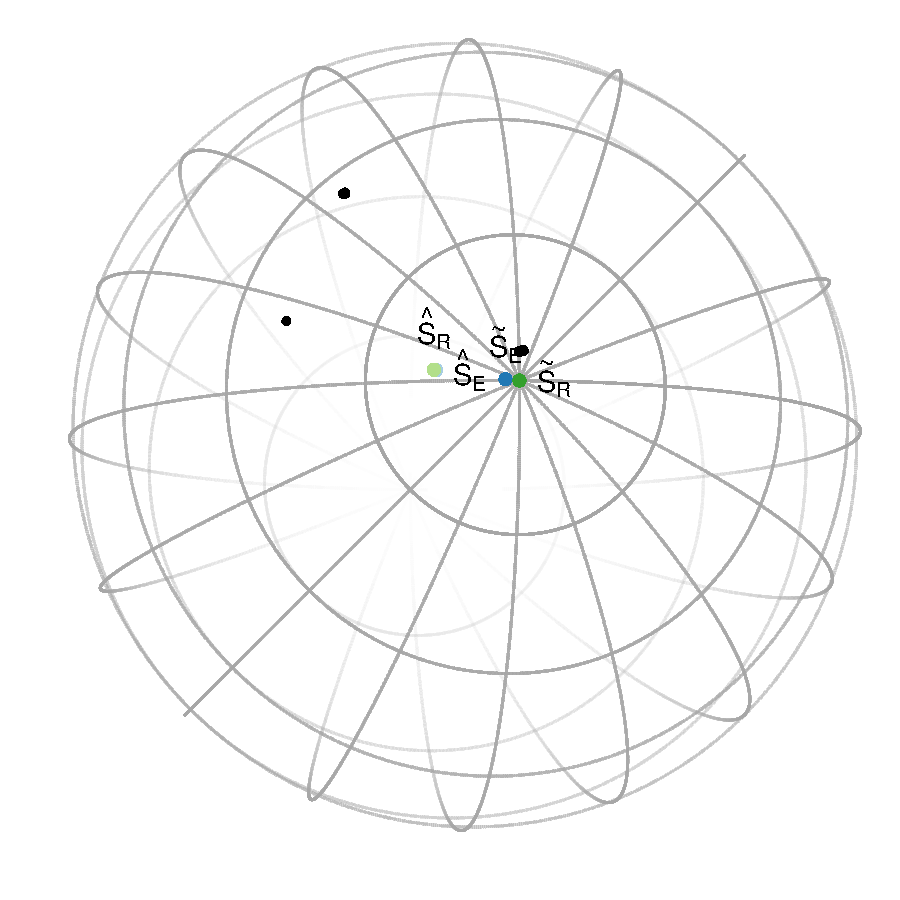
\includegraphics[width=.275\textwidth]{images/eyeball-1031-2.pdf} 
%%   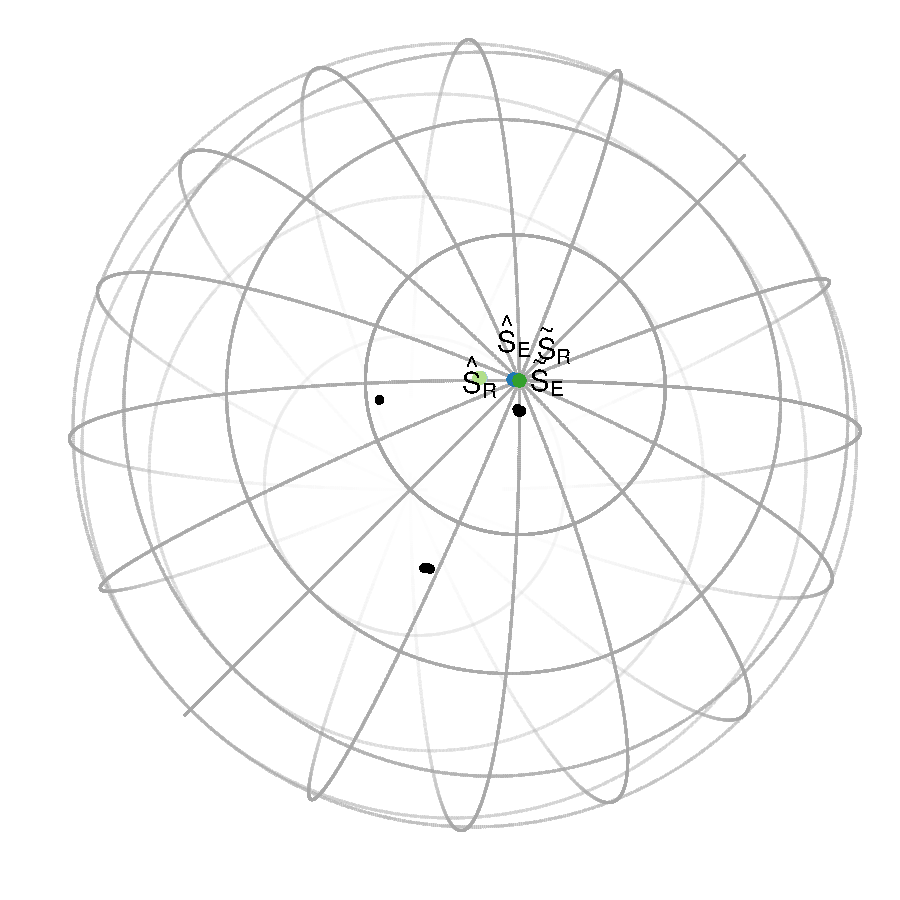
\includegraphics[width=.275\textwidth]{images/eyeball-1031-3.pdf} 
%%   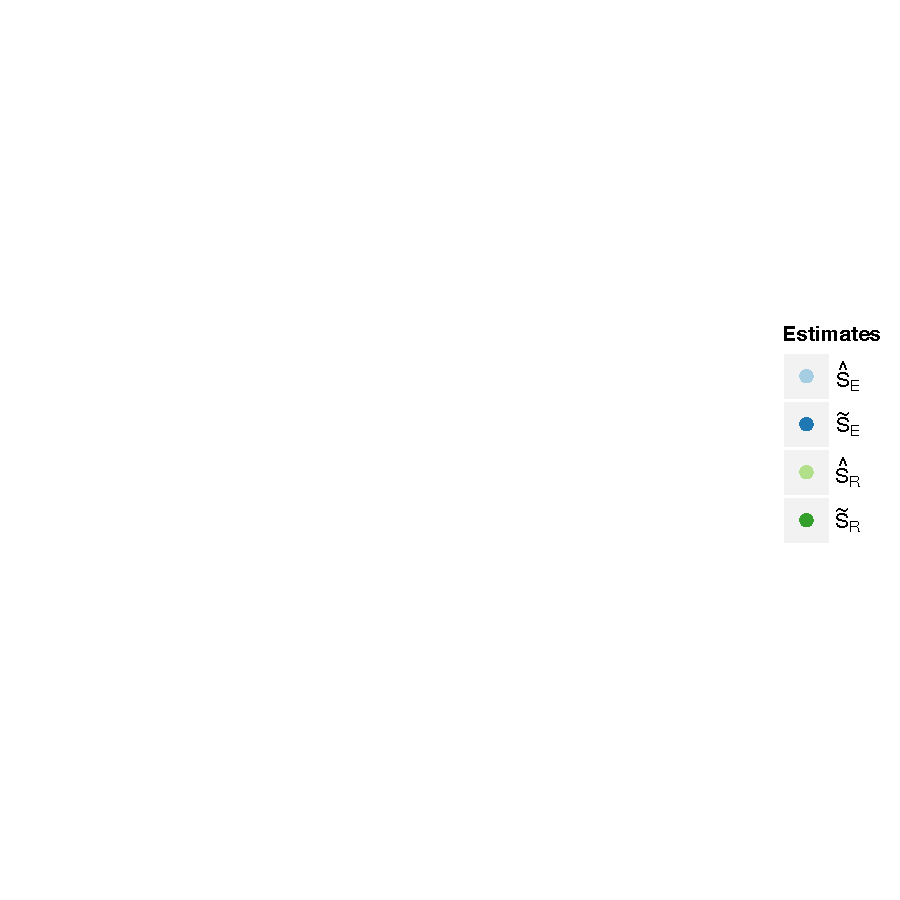
\includegraphics[height=.275\textwidth]{images/legend.pdf} 
%%   \caption{ \label{fig:eyeballs-1}Sphere plots of EBSD measurements at a single location. The data sample is shown as dark grey points, the estimates of the main direction are colored and labelled. The clustering of the results makes the existence  of several main directions  quite obvious. }
%%\end{figure}
%
%\begin{figure}[htbp] %  figure placement: here, top, bottom, or page
%   \centering
%   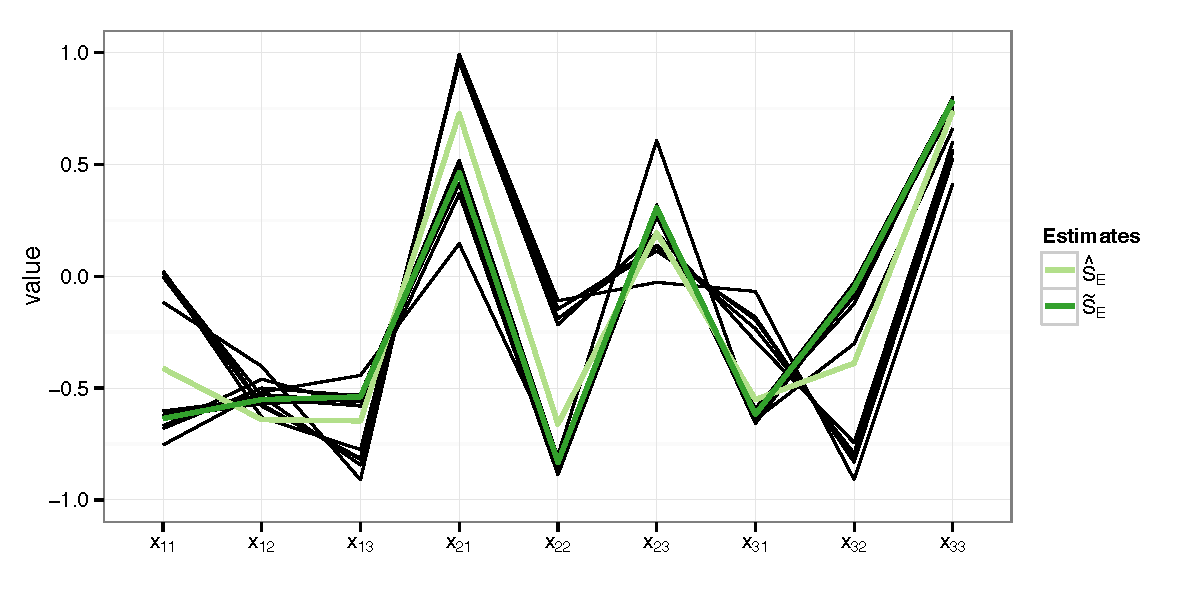
\includegraphics[width=.7\textwidth]{images/pcp.pdf} 
%   \caption{ \label{fig:pcp}Parallel coordinate plot of all nine coefficients of the rotation matrices in a single location. }
%\end{figure}
%
%>>>>>>> 2ae524a3512a18ca58f9808d9a1c66a11687f0c3

% !TEX root = Stanfill_CoDA.tex
\section{Recommendations and Conclusions}\label{sec:disc}

The scientific literature suggests a variety of approaches to estimate the central orientation $\bm S$ given a random sample of three-dimensional orientations from \eqref{eqn:1}. These approaches differ largely with respect to the geometry (Riemannian vs.~Euclidean) of estimation, assumptions about the underlying data-generating mechanism, and the choice of loss function when defining suitable estimators. The main goal of this paper was to explore the extent to which these choices affect the estimation of $\bm S$. 
Our simulation study showed that  the underlying data-generating mechanism guides our choice of loss function.  For the circular-von Mises-based model median-type estimators perform better while for the Cayley and matrix Fisher model the mean-type estimators show less estimation error and variability. As noted in Section~\ref{ch:intro} the applied sciences generally pursue estimation of $\bm S$ without considering the distributional underpinnings. Restricting ourselves to the three rotation distributions under consideration,  if indeed nothing is known about the underlying data-generating mechanism we suggest to use either median-type estimator, where the proposed median, the Euclidean based estimator $\ProjMedian$, emerges as a good overall choice. Its overall estimation error, even under mis-specification, will be much less than the potential estimation error resulting from either mean-type estimator. The extent to which all four estimators disagree depends on the variability in the rotation data; the estimators differ more when the circular variance $\nu$ is large and tend to agree more as the data become more concentrated.  
   
Further studies could be extended to include location estimation in non-symmetric distributional models for rotations as we considered common models for symmetric perturbations around $\bm S$ in \eqref{eqn:1}. Another important consideration is the extension of the studied point estimators to building confidence regions for the location parameter $\bm S$. One possibility would be resampling-based confidence regions, but this requires theoretical development for the estimator's sampling distributions and improvements in computing time before this can be practically implemented. \\

\section*{Supplementary Materials}

\begin{description}

\item[Supplementary material:] The relationship between $\Edist$ and $\Rdist$ is proven along with an extended look at the results. (PDF file)

\item[Rotations Code:] All the R code necessary to recreate the simulation results and plots shown in this paper. (.R file)

\end{description}

%\noindent \textbf{Acknowledgements:} The authors wish to thank Melissa Bingham and the Ames Laboratory for collecting and providing the EBSD data. We also gratefully acknowledge the suggestions made by the reviewers, the Associate Editor and Editor, all of which significantly improved the manuscript.

%=======
%% !TEX root = Stanfill_CoDA.tex
%\section{Recommendations and Conclusions}\label{sec:disc}
%
%The scientific literature suggests a variety of approaches to estimate the central orientation $\bm S$ given a random sample of three-dimensional orientations from \eqref{eqn:1}. These approaches differ largely with respect to the geometry (Riemannian vs.~Euclidean) in which the estimation is done, assumptions about the underlying data-generating mechanism and the choice of loss function when defining suitable estimators. The main goal of this paper was to explore the extent to which these choices affect the estimation of $\bm S$. 
%Our simulation study showed that  the underlying data-generating mechanism guides our choice of loss function.  For the circular-von Mises-based model median-type estimators perform better while for the Cayley and matrix Fisher model the mean-type estimators show less estimation error and variability. As noted in Section~\ref{ch:intro} the applied sciences generally pursue estimation of $\bm S$ without considering the distributional underpinnings. This can be a pitfall. Restricting ourselves to the three rotation distributions under consideration,  if indeed nothing is known about the underlying data-generating mechanism we suggest to use either median-type estimator, i.e. $\ProjMedian$ or $\GeomMedian$. The overall estimation error, even under mis-specification will be much less than the potential estimation error resulting from either mean-type estimator. The effect the geometry has on the precision of the estimates also depends on the underlying distributional model, however, to a smaller degree. %The Riemannian distance metric  $\Rdist$ is generally not recommended with a mean-type estimator due to the resulting increase in variability in the estimation errors. This fact holds across all three distributions  and is much expressed than for any of the other three estimators.
%In summary, the extent to which all four estimators disagree relative to each other depends on the circular variance $\nu$; the estimators differ more when $\nu$ is large and tend to agree more as the data become more concentrated.  
%   
%The scope of this study can be extended to other frequently encountered distributional models, especially because we restricted the simulation to symmetric perturbations around $\bm S$ in \eqref{eqn:1}. At least as important, if not even more, is the extension of the studied point estimators to interval estimators. The latter requires a significant improvement in computing time before it can be practically implemented. \\
%
%>>>>>>> 2ae524a3512a18ca58f9808d9a1c66a11687f0c3

\clearpage
\bibliography{bing}
%\clearpage
%\documentclass[12pt]{article}

%Technometrics specified margins:

% NOTE: To produce blinded version, replace "0" with "1" below.
\newcommand{\blind}{0}

% DON'T change margins - should be 1 inch all around.
\addtolength{\oddsidemargin}{-.5in}%
\addtolength{\evensidemargin}{-.5in}%
\addtolength{\textwidth}{1in}%
\addtolength{\textheight}{1.3in}%
\addtolength{\topmargin}{-.8in}%
\usepackage{psfrag,epsf,enumerate}

%\usepackage[margin=1.1in]{geometry}
\usepackage{color, amssymb, amsmath,bm,verbatim}
\usepackage{rotating, subfig, setspace, tikz}
\usepackage{graphicx, graphics, epsfig}
\usepackage{multirow,multicol}
\usepackage{natbib}
\newcommand{\tr}{{\mathbf{tr}}}
\newcommand{\rmk}{{\mathcal{K}}}
\newcommand{\I}{{\mathrm{I}}}
\newcommand{\E}{{\mathrm{E}}}
\newcommand{\B}{{\mathcal{B}}}
\newcommand{\bmo}{{\bm{o}}}
\newcommand{\R}{{\mathbb{R}}}
\newcommand{\cov}{{\mathrm{Cov}}}
\newcommand{\Log}{\text{Log}}
\newcommand{\M}{\mathcal{M}}
\newcommand{\refeq}[1]{{eq.~(\ref{#1})}}

\newcommand{\ProjMean}{{\widehat{\bm S}_E}}
\newcommand{\ProjMedian}{{\widetilde{\bm S}_E}}
\newcommand{\GeomMean}{{\widehat{\bm S}_R}}
\newcommand{\GeomMedian}{{\widetilde{\bm S}_R}}
\newcommand{\Rdist}{{d_R}}
\newcommand{\Edist}{{d_E}}

\DeclareMathOperator*{\argmax}{arg\,max}
\DeclareMathOperator*{\argmin}{arg\,min}
\newcommand{\blue}[1]{{\color{blue} #1}}
\newcommand{\red}[1]{{\color{red} #1}}
\newcommand{\green}[1]{{\color{green} #1}}
\newcommand{\hh}[1]{{\color{orange} #1}}

%\pagestyle{plain}
%\bibliographystyle{plainnat}
\bibliographystyle{abbrvnat}
\setcounter{section}{0}
\bibpunct{(}{)}{;}{a}{,}{;}
\graphicspath{{images/}}
%\setlength{\parindent}{0pt}
\begin{document}
\def\spacingset#1{\renewcommand{\baselinestretch}%
{#1}\small\normalsize} \spacingset{1}
%\setcounter{table}{4}
%\setcounter{figure}{9}
\appendix
\spacingset{1.45} % DON'T change the spacing!
\begin{center}
\Large \textbf{Online Supplemental Material}
\end{center}
\section{Riemannian versus Euclidean Distance in $SO(3)$}
\label{sec:appendix2}
\textit{Result.} For rotation matrices $\bm R_i\in SO(3)$ for $i=1,2,\ldots$ and distances $d_E$ and $d_R$ as defined in the main manuscript in equations (3) and (4), respectively,  it holds that 
\begin{equation}
\label{EvR}
\Edist(\bm R_1,\bm R_2)=2^{3/2}\sin\left(\frac{\Rdist(\bm{R}_1,\bm{R}_2)}{2}\right)
.
\end{equation}
%\begin{figure}[h!]
%\begin{center}
%\begin{tikzpicture}[scale=.9]
%%\draw (0,0) circle (4cm);
%\draw (0,0) node {$\bullet$};
%\draw (3.464102,2) node[anchor =  west]{$\bm R_1\bm v$};
%\draw [->] (0,0)--(4,0);
%%\draw [->] (4,0) arc (0:30:4cm);
%\draw (2,0) node[anchor = north]{$\bm v=(0,1)^\top$};
%\draw (-2,3.46) node[anchor = south east]{$\bm R_2\bm v$};
%\draw [line width=.75mm] (3.464102,2) arc (30:120:4cm);
%\draw[line width=.75mm, color=gray] (-2,3.46)--(3.464102,2);
%\draw [->](0,0) -- (-2,3.464102);
%\draw [->](0,0)--(3.464102,2);
%\draw (1,3.66) node[anchor= south west]{$\Rdist (\bm R_1,\bm R_2)$};
%\draw (-1,1.75) node[anchor= south west]{$\Edist (\bm R_1,\bm R_2)$};
%\draw (0,0) circle (4cm);
%\draw (0,0) node {$\bullet$};
%\draw (0,0)--(4,0) node[anchor =  west]{$o_1$};
%\draw (4,0) node[anchor =  west]{$\bm R_1$};
%\draw (0,0)--(-2,3.46) node[anchor = south east]{$o_2$};
%\draw (-2,3.46) node[anchor = south east]{$\bm R_2$};
%\draw[line width=.75mm] (4,0) arc (0:120:4cm);
%\draw[line width=.75mm, color=gray] (-2,3.46)--(4,0);
%\draw (0,0)--(2,3.46) node[anchor= south west]{$\alpha$};
%\draw (2,3.46) node[anchor= south west]{$\Rdist (\bm R_1,\bm R_2)$};
%\draw (-1.25,0.73) node[anchor= south west]{$\Edist (\bm R_1,\bm R_2)$};
%\draw (3/8,.7)[->] arc (60:120:.75cm);
%\draw (0,1.2) node {$\frac{\alpha}{2}$};
%\draw (0,2.8) node {$\frac{\beta}{2}$};
%\draw (2,0) node[anchor=north]{1};
%\end{tikzpicture}
%\end{center}
%\vspace{-.25cm}
%\caption{An illustration of the Euclidean and Riemannian distance metric on $SO(2)$. To simplify the visualization we use $SO(2)$ in place of $SO(3)$.   $\bm R_1$, $\bm R_2$ are $2\times2$ rotation matrices in $SO(2)$, where $\bm R_1\bm v$ and $\bm R_2\bm v$ are points on the $\mathbb R^2$ unit circle after rotating $\bm v = (0,1)^{\top}$ by  $\bm R_1$ and $\bm R_2$, respectively.  $\Rdist (\bm R_1,\bm R_2)$ is displayed by the curved line (black), $\Edist (\bm R_1,\bm R_2)$ by the straight line (gray).}
%\label{fig:dEvsdG2} 
%\end{figure}

%\noindent In Figure \ref{fig:dEvsdG2} the Riemannian distance between $\bm R_1$ and $\bm R_2\in SO(2)$ is given by $\Rdist(\bm R_1,\bm R_2)$ and is indicated with the thick black arc.  The Euclidean distance is given by $\Edist(\bm R_1,\bm R_2)$ and is indicated by the straight gray line.  Using geometry it is clear that half of the Euclidean distance is the sine of half of the Riemannian distance, i.e.
%\[
%\Edist(\bm R_1,\bm R_2)=2\sin\left(\frac{\Rdist(\bm R_1,\bm R_2)}{2}\right).
%\]

%\noindent We claim that this can be extended to $\bm R_1,\bm R_2 \in SO(3)$ as 
%\begin{equation}\label{EvR}
%\Edist (\bm{R}_1,\bm{R}_2)=2^{3/2}\sin\left(\frac{\Rdist(\bm{R}_1,\bm{R}_2)}{2}\right)
%\end{equation}

\noindent \textit{Proof:} For two rotations $\bm{R}_1,\bm{R}_2\in SO(3)$ recall that if $\tr(\bm R_1^\top\bm R_2)=1+2\cos(r)$ then $|r|=\Rdist(\bm R_1,\bm R_2)$.  When $|r|=0$, the statement in \eqref{EvR} follows directly.  Consider the case $|r|>0$.  By definition we know
\begin{align*}
\Edist (\bm R_1,\bm R_2)^2
&=||\bm R_1-\bm R_2||_F^2\\
&=\tr\left[(\bm R_1-\bm R_2)^\top(\bm R_1-\bm R_2)\right]\\
%&=\tr\left[(\bm R_1^\top-\bm R_2^\top)(\bm R_1-\bm R_2)\right]\\
&=\tr\left[\bm R_1^\top\bm R_1+\bm R_2^\top\bm R_2-\bm R_2^\top\bm R_1-\bm R_1^\top\bm R_2\right]\\
&=\tr\left[2\bm{I}-\bm R_2^\top\bm R_1-\bm R_1^\top\bm R_2\right]\\
&=2\tr(\bm{I})-\tr(\bm R_2^\top\bm R_1)-\tr(\bm R_1^\top\bm R_2)\\
&=6-2\tr(\bm R_1^\top\bm R_2)\\
%&=6-2(1+2\cos(r))\\
&=6-2-4\cos(|r|)\\
&=8\left(\frac{1-\cos(|r|)}{2}\right)\\
&=8\sin^2\left(\frac{|r|}{2}\right)\\
&=\left[2^{3/2}\sin\left(\frac{|r|}{2}\right)\right]^2\\
&=\left[2^{3/2}\sin\left(\frac{\Rdist(\bm R_1,\bm R_2)}{2}\right)\right]^2.
\end{align*}
Taking square root on both sides gives \eqref{EvR}.

\section{Sampling Processes}
In the following subsection we will briefly illustrate how a sample of random rotations from each of the three rotational distributions (circular-von Mises-based, Cayley and matrix-Fisher) is obtained for the purpose of the simulation study.
\label{sec:appendix1}
\subsection{Circular-von Mises-based distribution}

To simulate a random sample of rotation angles from the circular-von Mises-based distribution we follow the  algorithm proposed by Best and Fisher (1979).  The algorithm is available in the IMSL Library (1991) and is implemented as follows.  Let $\mu=0$ denote the mean of the target angular distribution and $\kappa$ its concentration parameter.  We define constants $a, b$ and $d$ as
$a\equiv 1+\sqrt{1+4\kappa^2},\quad b\equiv(a-\sqrt{2a}),\quad d\equiv(1+b^2)/2b.$
In steps one, two and four we generate three new observations $u_1$, $u_2$ and $u_3$,  each from a uniform distribution defined over the interval $(0,1)$. 
\begin{enumerate}
\item Set $z=\cos(\pi u_1)$, $f=(1+dz)/(z+d)$ and $c=\kappa(d-f)$.
\item If $c(2-c)-u_2>0$ go to step 4.
\item If $\log(c/u_2)+1-c<0$ return to step 1.
\item Set $r=\text{sign}(u_3-0.5)\cos^{-1}(f).$
\end{enumerate}
It follows that  $r$ is distributed according to the circular-von Mises$(\kappa)$ distribution.

\subsection{Cayley distribution}%\hfill

To simulate rotation angles from a Cayley distribution we make use of a result given in Le{\'o}n et al., (2006). If the angle $r$ follows a Cayley distribution it holds that $\frac{1+\cos r}{2} \sim \text{Beta}(\kappa+1/2, 3/2)$.  Hence, angles following the Cayley distribution can be simulated through composition: 
\begin{enumerate}
\item Generate $Z\sim$Bernoulli(0.5) and set  $Y=1-2Z.$
\item Independently generate $X\sim$ Beta$(\kappa+1/2, 3/2).$
\item Set $r= \frac{Y}{2}\cos^{-1}(2X-1).$
\end{enumerate}
Angles $r$ simulated in this fashion follow a Cayley$(\kappa)$ distribution.

\subsection{matrix Fisher distribution}%\hfill

Simulation from the matrix Fisher distribution is achieved through a rejection algorithm.  Let  $\mathrm{C_F}(r|\kappa)$ denote the matrix Fisher density.% as given in Table~\ref{tab:ang.dens}. %and $Y\sim$ Uniform$(-\pi,\pi]$.

\begin{enumerate}
\item Define $M=\frac{1}{2\kappa}e^{2\kappa - 1}\frac{1}{\mathbf{I}_0(2\kappa)-\mathbf{I}_1(2\kappa)}.$
\item Generate $U\sim$ Uniform$(0,1)$ and $Y\sim$ Uniform$(-\pi,\pi]$, where $U$ and $Y$ are independent.
\item If $U<\frac{1}{M}\mathrm{C_F}(Y|\kappa)$, accept $Y$; otherwise return to step (2).
\end{enumerate}

%\subsection{Rotation Matrix Formulation}
%
%Given a set of randomly generated angles of rotation $r_1,\ldots, r_n$, the rotation matrix formulation following from:
%\begin{enumerate}
%\item Generate a point uniformly on the unit sphere
%$$\bm{U}=(u_1,u_2,u_3)^\top=(\sin\theta\cos\phi,\sin\theta\sin\phi,\cos\theta)^\top$$
%where  $0\leq \theta\leq \pi$ and $0\leq \phi\leq 2\pi$.
%\item Given an angle of rotation,$r_i$ , generated as described above from an angular distribution symmetric about 0 and with concentration $\kappa$ rotate $\bm{I}$ about $\bm{U}$ by $r_i$ radians.
%\end{enumerate}


\section{Additional Simulation Study Results}
\label{sec:appendix3}
We expand on some of the results given in Section~5 of the main manuscript by providing additional numerical results to support graphical displays as well as to further clarify the relationship between the different estimators.

\noindent Figure~4 of the main manuscript showed boxplots of the estimation errors for a each of a 1,000 samples of size $n=100$ for all three distributions and choices of the circular variance $\nu$.  We accompany this figure with Table~\ref{tab:alldN100}, which provides numerical summaries of the errors displayed in each boxplot showing the mean estimation error $\overline{\Rdist}(\bm{S}, \widehat{\bm{S}})$ in the $1,000$ simulation runs, the estimated standard error $SE(\overline{\Rdist})$ and the estimated $RMSE$ for each estimator.  Although the boxplots of the estimation errors look very similar in Figure~4, the estimated standard errors in Table \ref{tab:alldN100} suggest that on average some of the estimators differ significantly.  


\begin{table}[h!]
\caption{Mean estimation error, respective standard error and RMSE for $n=100$ based on 1,000 simulation runs. Despite skewness in some of the plotted error distributions the \textit{median estimation error} was quantitatively similar to the mean estimation error and therefore is not reported.
}  
\label{tab:alldN100}
\centering
\scalebox{.85}{
\begin{tabular}{ccccccccccc}
\hline
		&&\multicolumn{3}{c}{\textbf{Cayley}} & \multicolumn{3}{c}{\textbf{matrix Fisher}}  & \multicolumn{3}{c}{\textbf{circular-von Mises}}\\[.15cm] 
  $\nu$ & Estimator && $\overline{\Rdist}(\bm{S}, \widehat{\bm{S}})$  $SE(\overline{\Rdist})$ & RMSE && $\overline{\Rdist}(\bm{S}, \widehat{\bm{S}})$ $SE(\overline{\Rdist}$) & RMSE && $\overline{\Rdist}(\bm{S}, \widehat{\bm{S}})$ $SE(\overline{\Rdist})$ & RMSE \\ \hline
  \hline
 \multirow{4}{*}{0.25} 
 	& $\GeomMean$ && 0.0690 (0.0009) & 0.0752 && 0.0699 (0.0010) & 0.0761 && 0.0744 (0.0010) & 0.0811 \\ 
  	& $\ProjMean$ && 0.0698 (0.0009) & 0.0759 && 0.0695 (0.0009) & 0.0756 && 0.0617 (0.0008) & 0.0671 \\ 
  	& $\GeomMedian$ && 0.0769 (0.0010) & 0.0834 && 0.0747 (0.0010) & 0.0813 && 0.0269 (0.0005) & 0.0310 \\ 
   	&$\ProjMedian$ && 0.0791 (0.0011) & 0.0858 && 0.0766 (0.0010) & 0.0832 && 0.0256 (0.0005) & 0.0296 \\ \hline
  	 \multirow{4}{*}{0.50} 
	&$\GeomMean$ && 0.1086 (0.0014) & 0.1174 && 0.1121 (0.0015) & 0.1219 && 0.1279 (0.0018) & 0.1406 \\ 
  	& $\ProjMean$ && 0.1129 (0.0015) & 0.1222 && 0.1054 (0.0014) & 0.1143 && 0.0894 (0.0012) & 0.0976 \\ 
  	& $\GeomMedian$ && 0.1210 (0.0016) & 0.1313 && 0.1113 (0.0015) & 0.1211 && 0.0426 (0.0008) & 0.0491 \\ 
  	& $\ProjMedian$ && 0.1295 (0.0017) & 0.1407 && 0.1160 (0.0016) & 0.1262 && 0.0379 (0.0007) & 0.0438 \\\hline
  	 \multirow{4}{*}{0.75} 
	& $\GeomMean$ && 0.1398 (0.0018) & 0.1514 && 0.1703 (0.0045) & 0.2225 && 0.2039 (0.0028) & 0.2221 \\ 
  	& $\ProjMean$ && 0.1567 (0.0020) & 0.1695 && 0.1462 (0.0020) & 0.1588 && 0.1276 (0.0017) & 0.1388 \\ 
  	& $\GeomMedian$ && 0.1597 (0.0021) & 0.1729 && 0.1527 (0.0021) & 0.1660 && 0.0687 (0.0012) & 0.0792 \\ 
  	& $\ProjMedian$ && 0.1847 (0.0024) & 0.2000 && 0.1597 (0.0022) & 0.1736 && 0.0547 (0.0010) & 0.0628 \\ 
   \hline
\end{tabular}}
\end{table}

\noindent To establish significant differences more formally we conducted \textit{matched pair} $t$-\textit{tests} (two-sided) for all six pairwise comparisons of the four estimators within a specific simulation setting.  The results are given in Table~\ref{tab:pvalues}. We tested the null hypothesis that the difference in the resulting estimates, on average, is zero against the alternative hypothesis that the difference, on average, is non-zero.  Because differences in the estimation error seem less obvious for the Cayley and matrix-Fisher distribution we conducted tests for both distributions for samples of size 10 and 100 and circular variances of 0.25 and 0.75. 
We suspect that a \textit{matched pair} $t$-\textit{test} based on all of the $B=1,000$ simulations will likely yield statistically significant differences that are an artifact of the size of $B$ as opposed to meaningful and practical differences we also provide the results for (arbitrary) choices of $B=50$ and $B=100.$ For $B=50$ and $B=100$ we base the test on the estimation results for $B$ randomly selected simulation runs and repeated this process 100 times. The reported \textit{p-value} then corresponds to the average \textit{p-value} of these 100 runs. For $B=1,000$ the reported \textit{p-value} is based on all original 1,000 runs. 
We further adjusted the level of significance within each row of Table~\ref{tab:pvalues} using 
a Bonferroni correction for multiple comparisons and therefore, within a set of all six pairwise comparisons, consider \textit{p-values} less than $0.05\div6=0.0083$.  We chose the Bonferroni adjustment because of its simplicity. \\

\noindent From Table \ref{tab:pvalues} we can conclude that for the Cayley distribution the choice of geometry is important when using median type estimators (column 1), but not as important for mean type estimators (column 2) unless the circular variance and sample size is large.  For a given geometry, the difference between mean and median type estimator depends on the level of variability in the data as is the case in the one dimension case (columns 3 and 4).  As for the matrix-Fisher distribution, the choice of estimator does not appear to be overtly significant for any sample size or circular variance.  This is likely due to the fact that this distribution closely resembles the normal distribution on the range $[-\pi,\pi)$ in which case the mean and median are equivalent.

\begin{table}[h!]
\caption{P-values for matched pair t-tests on the average differences between estimators.  Unless $B$ equals 1,000 the reported \textit{p-values} correspond to the average of 100 \textit{p-values} based on random samples of size $B$ from the 1,000 simulation runs.  We omitted samples in the calculations for which the algorithm to compute $\widehat{\bm S}$ did not converge were omitted.}
\label{tab:pvalues}
\begin{center}
\scalebox{.89}{
\begin{tabular}{ccccrrrrrr}
  \hline\\[-4pt]
 Distribution & $\nu$ & $n$ & $B$ &$\ProjMedian-\GeomMedian$ & $\ProjMean-\GeomMean$ & $\ProjMean-\ProjMedian$ & $\GeomMean-\GeomMedian$ & $\ProjMean-\GeomMedian$ & $\ProjMedian-\GeomMean$ \\ 
 \hline\hline
 \multirow{12}{*}{Cayley} & \multirow{6}{*}{0.25} & \multirow{3}{*}{10} & 50 & \textbf{0.0012} & 0.4106 & 0.0181 & 0.0591 & 0.0385 & 0.0298 \\ 
  &  &  & 100 & $<$\textbf{0.0001} & 0.3438 & \textbf{0.0004} & \textbf{0.0040} & \textbf{0.0022} & \textbf{0.0008} \\ 
  &  &  & 1000 & $<$\textbf{0.0001} & \textbf{0.0022} & $<$\textbf{0.0001} & $<$\textbf{0.0001} & $<$\textbf{0.0001} & $<$\textbf{0.0001} \\ \cline{3-10}
  &  & \multirow{3}{*}{100} & 50 & $<$\textbf{0.0001} & 0.2937 & 0.0110 & 0.0360 & 0.0248 & 0.0179 \\ 
  &  &  & 100 & $<$\textbf{0.0001} & 0.1356 & \textbf{0.0002} & \textbf{0.0012} & \textbf{0.0007} & \textbf{0.0003} \\ 
  &  &  & 1000 &$<$\textbf{0.0001} & $<$\textbf{0.0001} & $<$\textbf{0.0001} & $<$\textbf{0.0001} & $<$\textbf{0.0001} & $<$\textbf{0.0001} \\ \cline{2-10}
  &  \multirow{6}{*}{0.75}& \multirow{3}{*}{10} & 50 & \textbf{0.0001} & 0.0343 & \textbf{0.0008} & 0.0376 & 0.3306 & \textbf{0.0005} \\ 
  &  &  & 100 & $<$\textbf{0.0001} & \textbf{0.0015} & $<$\textbf{0.0001} & \textbf{0.0018} & 0.2848 & $<$\textbf{0.0001} \\ 
  &  &  & 1000 & $<$\textbf{0.0001} & $<$\textbf{0.0001} & $<$\textbf{0.0001} & $<$\textbf{0.0001} & $<$\textbf{0.0001} & $<$\textbf{0.0001} \\ \cline{3-10}
  &  & \multirow{3}{*}{100} & 50 & $<$\textbf{0.0001} & \textbf{0.0017} & \textbf{0.0001} & \textbf{0.0024} & 0.3292 &$<$\textbf{0.0001} \\ 
  &  &  & 100 & $<$\textbf{0.0001} & $<$\textbf{0.0001} & $<$\textbf{0.0001} & $<$\textbf{0.0001} & 0.3046 & $<$\textbf{0.0001} \\ 
  &  &  & 1000 & $<$\textbf{0.0001} & $<$\textbf{0.0001} & $<$\textbf{0.0001} & $<$\textbf{0.0001} & $<$\textbf{0.0001} & $<$\textbf{0.0001} \\[5pt] \hline\\[-4pt]
  & \multirow{6}{*}{0.25} & \multirow{3}{*}{10} & 50 & 0.0116 & 0.5032 & 0.0791 & 0.2135 & 0.1338 & 0.1394 \\ 
  &  &  & 100 & \textbf{0.0012} & 0.3815 & 0.0213 & 0.1171 & 0.0540 & 0.0586 \\ 
  &  &  & 1000 & $<$\textbf{0.0001} & \textbf{0.0008} & $<$\textbf{0.0001} & $<$\textbf{0.0001} & $<$\textbf{0.0001} & $<$\textbf{0.0001} \\ \cline{3-10}
  &  & \multirow{3}{*}{100} & 50 & \textbf{0.0072} & 0.4314 & 0.0773 & 0.2313 & 0.1200 & 0.1620 \\ 
  &  &  & 100 & \textbf{0.0001} & 0.4250 & \textbf{0.0047} & 0.0603 & 0.0143 & 0.0244 \\ 
  matrix-&  &  & 1000 & $<$\textbf{0.0001} & 0.0303 & $<$\textbf{0.0001} & $<$\textbf{0.0001} & $<$\textbf{0.0001} & $<$\textbf{0.0001} \\ \cline{2-10}
  Fisher& \multirow{6}{*}{0.75} & \multirow{3}{*}{10} & 50 & 0.1027 & 0.1864 & 0.0842 & 0.3483 & 0.3509 & 0.4652 \\ 
  &  &  & 100 & 0.0205 & 0.0730 &\textbf{0.0075} & 0.2476 & 0.1666 & 0.5001 \\ 
  &  &  & 1000 & $<$\textbf{0.0001} & $<$\textbf{0.0001} & $<$\textbf{0.0001} & $<$\textbf{0.0001} & $<$\textbf{0.0001} & 0.1050 \\ \cline{3-10}
  &  & \multirow{3}{*}{100} & 50 & 0.1475 & 0.0586 & 0.0559 & 0.2005 & 0.2296 & 0.4738 \\ 
  &  &  & 100 & 0.0419 & \textbf{0.0081} & \textbf{0.0056} & 0.0747 & 0.0768 & 0.4437 \\ 
  &  &  & 1000 & $<$\textbf{0.0001} & $<$\textbf{0.0001} & $<$\textbf{0.0001} & $<$\textbf{0.0001} & $<$\textbf{0.0001} & 0.0198 \\ 
   \hline
\end{tabular}}
\end{center}
\end{table}

\noindent Figure \ref{fig:NBoxes} illustrates the behavior of the estimators as a function of the sample size. Results are displayed for  $\nu=0.75$ at each sample size. As to be expected, the estimation error decreases as the sample size increases for all three distributions. For small samples, e.g., $n=10$, the estimator exhibiting the largest amount of variability is the geodesic mean $\GeomMean$. This behavior is consistent for all three distributions.  While the estimator's variability lessens considerably for the Cayley and matrix Fisher distribution as $n$ increases, the estimator remains the most variable estimator for the circular-von Mises-based distribution.  A possible explanation for this behavior is that the algorithm to estimate $\GeomMean$ uses a random sample point in its initiating step.  For small samples or samples with several extreme observations it is likely to start the algorithm far from the true center, which in turn may cause the algorithm to get stuck in a local minimum and to fail to converge globally.  In practice we suggest the algorithm be started at some other location estimate of $\bm S$ such as the $\ProjMean$. In simulations where $\ProjMean$ was used as a starting point for the algorithm we observed  similar results with less variability in the estimates of $\GeomMean$, but for the purpose of a fair comparison in this study we started the algorithm at a random sample point.


\begin{figure}[h!]
\centering
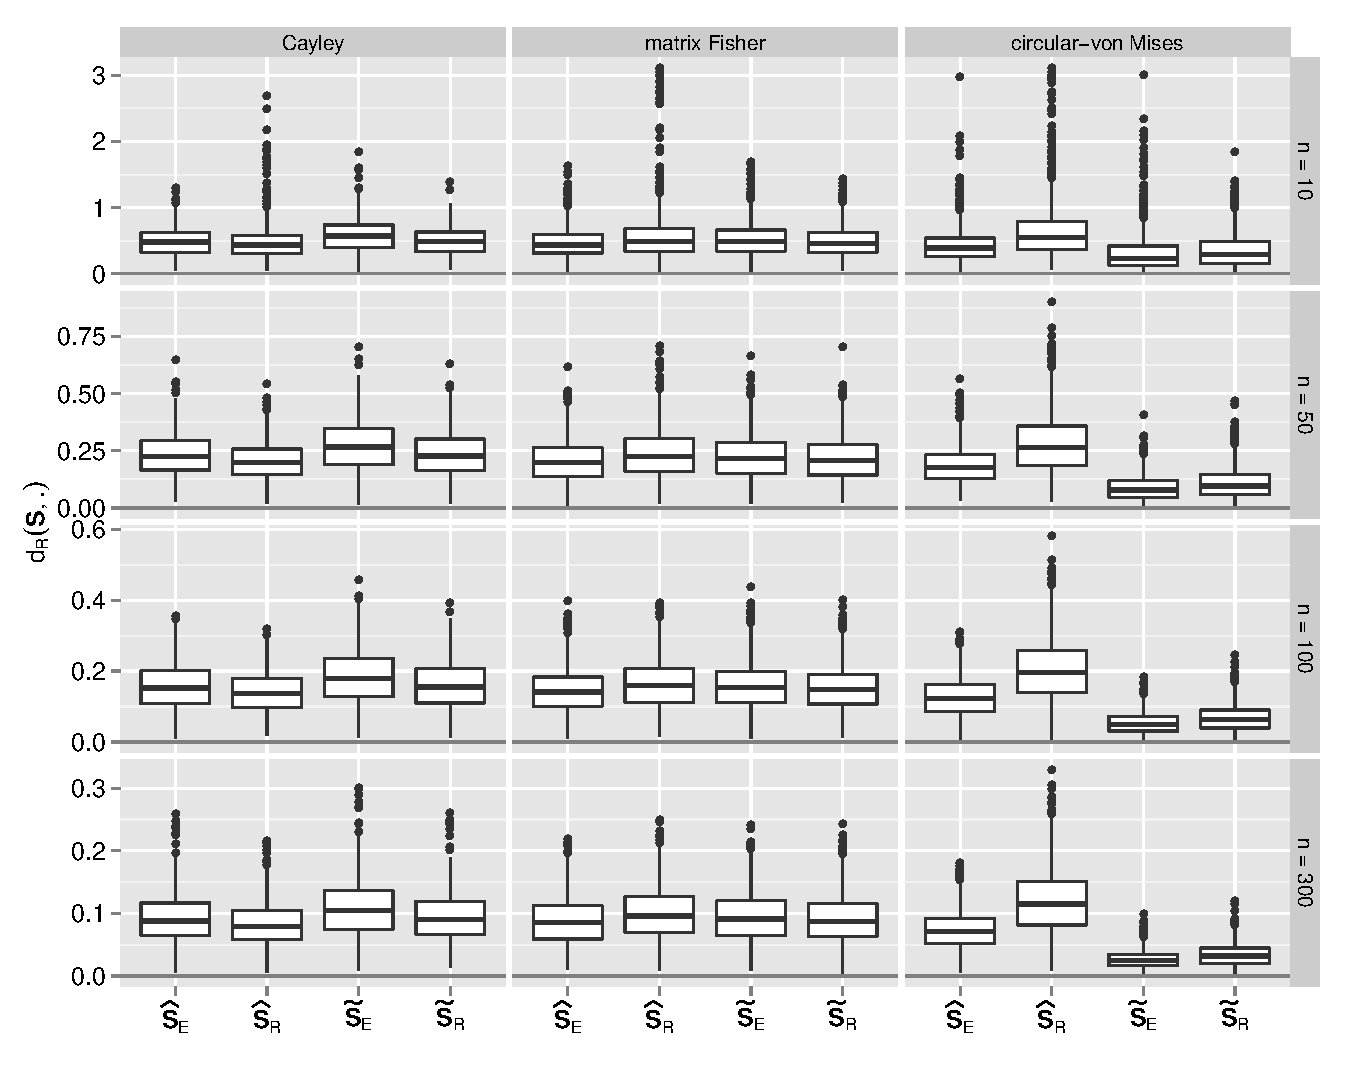
\includegraphics[width=1\textwidth]{Nu75AllNBoxes.pdf}
\caption{Boxplots of the estimation error for each rotation distribution and level of $n$,  $\nu=0.75$.}
\label{fig:NBoxes}
\end{figure}


\noindent In Figure 7 of the main manuscript we examined how the choice of geometry (Riemannian versus Euclidean) affected the estimation error under both types of loss functions $L
_1$ and $L_
2$.  Tables~\ref{tab:percL1} and \ref{tab:percL2} support Figure 7 with an exact count (expressed as a percentage) of how often $\Rdist$ resulted in a smaller estimation error than $\Edist$.  Additionally, we give the average amount by which the $\Rdist-$ and $\Edist-$based estimates deviate from one another (along with a standard error estimate).  We denote the latter quantity by $\bar\delta$ where  $\delta=\Rdist(\ProjMedian,\bm S)-\Rdist(\GeomMedian,\bm S)$.   

\begin{table}[h]
\caption{Average reduction in estimation error by using $\GeomMedian$ instead of $\ProjMedian$, $\delta=\Rdist(\ProjMedian,\bm S) - \Rdist(\GeomMedian,\bm S)$ with standard error and percentage of samples for which $\Rdist(\GeomMedian,\bm S) < \Rdist(\ProjMedian,\bm S)$.}
\label{tab:percL1}
\centering
\scalebox{0.92}{
\begin{tabular}{crccccccccc}
  \hline
  %&&&\multicolumn{3}{c}{} & &\multicolumn{3}{c}{\textbf{matrix} } &&\multicolumn{3}{c}{\textbf{circular-}}\\
    &&&\multicolumn{2}{c}{\textbf{Cayley}} & &\multicolumn{2}{c}{\textbf{matrix Fisher}} & &\multicolumn{2}{c}{\textbf{circular-von Mises}}\\ 
\rule[2mm]{0mm}{3mm} 
  $\nu$&  $n$ && $\bar{\delta}$ (SE) & \% & & $\bar{\delta}$ (SE) & \% & & $\bar{\delta}$ (SE) & \% \\ 
  \hline \hline
\multirow{4}{*}{0.25}  
 &    10 && 0.0078 (0.0004) & 0.7430 && 0.0060 (0.0004) & 0.7250 && -0.0053 (0.0006) & 0.3280 \\ 
 &    50 && 0.0031 (0.0001) & 0.7830 && 0.0024 (0.0001) & 0.6970 && -0.0018 (0.0001) & 0.3270 \\ 
 &   100 && 0.0022 (0.0001) & 0.7890 && 0.0018 (0.0001) & 0.7120 && -0.0013 (0.0001) & 0.3080 \\ 
 &   300 && 0.0012 (0.0001) & 0.7810 && 0.0010 (0.0001) & 0.7110 && -0.0008 (0.0001) & 0.2840 \\
\hline
\multirow{4}{*}{0.50}   
  &    10 && 0.0315 (0.0016) & 0.7720 && 0.0171 (0.0017) & 0.6620 && -0.0192 (0.0020) & 0.3350 \\ 
  &    50 && 0.0126 (0.0005) & 0.8110 && 0.0055 (0.0006) & 0.6200 && -0.0081 (0.0005) & 0.2820 \\ 
  &   100 && 0.0085 (0.0003) & 0.8090 && 0.0047 (0.0004) & 0.6600 && -0.0047 (0.0003) & 0.3020 \\ 
  &   300 && 0.0049 (0.0002) & 0.8040 && 0.0024 (0.0002) & 0.6580 && -0.0027 (0.0001) & 0.2550 \\ 
\hline
\multirow{4}{*}{0.75}   
  &    10 && 0.0895 (0.0042) & 0.8210 && 0.0340 (0.0040) & 0.6330 && -0.0396 (0.0062) & 0.3220 \\ 
  &    50 && 0.0366 (0.0011) & 0.8660 && 0.0093 (0.0013) & 0.5970 && -0.0213 (0.0011) & 0.2380 \\ 
  &   100 && 0.0250 (0.0008) & 0.8580 && 0.0069 (0.0009) & 0.6030 && -0.0140 (0.0007) & 0.2400 \\ 
  &   300 && 0.0140 (0.0004) & 0.8500 && 0.0033 (0.0005) & 0.5890 && -0.0072 (0.0003) & 0.2180 \\   \hline
\end{tabular}}
\end{table}

\begin{table}[h!]
\caption{Average reduction in estimation error by using $\GeomMean$ instead of $\ProjMean$, $\delta=\Rdist(\ProjMean,\bm S) - \Rdist(\GeomMean,\bm S)$ with standard error and percentage of samples for which $\Rdist(\GeomMean,\bm S) < \Rdist(\ProjMean,\bm S)$.}  \label{tab:percL2}
\centering
\scalebox{0.92}{
\begin{tabular}{crcccccccccccc}
  \hline
  %& &&\multicolumn{3}{c}{} & &\multicolumn{3}{c}{\textbf{matrix} } &&\multicolumn{3}{c}{\textbf{circular-}}\\
    &&&\multicolumn{2}{c}{\textbf{Cayley}} & &\multicolumn{2}{c}{\textbf{matrix Fisher}} & &\multicolumn{2}{c}{\textbf{circular-von Mises}}\\ 
\rule[2mm]{0mm}{3mm} 
  $\nu$&  $n$ && $\bar{\delta}$ (SE) & \% & & $\bar{\delta}$ (SE) & \% & & $\bar{\delta}$ (SE) & \% \\  
  \hline \hline
\multirow{4}{*}{0.25} 
 &    10 && 0.0011 (0.0004) & 0.5210 && -0.0016 (0.0005) & 0.4500 && -0.0344 (0.0030) & 0.1280 \\ 
 &    50 && 0.0007 (0.0002) & 0.5310 && -0.0011 (0.0003) & 0.4350 && -0.0156 (0.0007) & 0.2090 \\ 
 &   100 && 0.0007 (0.0001) & 0.5650 && -0.0004 (0.0002) & 0.4690 && -0.0126 (0.0005) & 0.2010 \\ 
 &   300 && 0.0005 (0.0001) & 0.5880 && -0.0003 (0.0001) & 0.4860 && -0.0070 (0.0003) & 0.2390 \\\hline
\multirow{4}{*}{0.50}  
 &    10 && 0.0099 (0.0013) & 0.5920 && -0.0178 (0.0027) & 0.4340 && -0.1011 (0.0051) & 0.1570 \\ 
  &    50 && 0.0069 (0.0006) & 0.6450 && -0.0107 (0.0011) & 0.3920 && -0.0545 (0.0018) & 0.1450 \\ 
  &   100 && 0.0043 (0.0004) & 0.6420 && -0.0067 (0.0008) & 0.3930 && -0.0385 (0.0013) & 0.1620 \\ 
  &   300 && 0.0025 (0.0002) & 0.6420 && -0.0040 (0.0004) & 0.3930 && -0.0234 (0.0007) & 0.1570 \\ \hline
\multirow{4}{*}{0.75}  
  &    10 && 0.0163 (0.0062) & 0.6680 && -0.0958 (0.0105) & 0.3570 && -0.2101 (0.0113) & 0.1710 \\ 
  &    50 && 0.0257 (0.0012) & 0.7410 && -0.0356 (0.0045) & 0.3380 && -0.0955 (0.0032) & 0.1500 \\ 
  &   100 && 0.0169 (0.0009) & 0.7350 && -0.0240 (0.0043) & 0.3460 && -0.0763 (0.0021) & 0.1110 \\ 
  &   300 && 0.0091 (0.0005) & 0.7280 && -0.0124 (0.0009) & 0.3440 && -0.0446 (0.0012) & 0.1270 \\
   \hline
\end{tabular}}
\end{table}



%\begin{table}[h!]
%\caption{Results from an analysis of variance on the log transformed error data for $n=100$ and $\nu=0.25$ and treating distributions as blocks.  From this we can conclude that there is a statistically significant difference between the estimators.}
%\begin{center}
%\begin{tabular}{lrrrrr}
%  \hline
% & Df & Sum Sq & Mean Sq & F value & Pr($>$F) \\ 
%  \hline
%Distribution       & 2 & 927.61 & 463.80 & 1371.56 & $<1\times 10^{-5}$ \\ 
%Estimator   & 3 & 228.43 & 76.14 & 225.17 & $<1\times 10^{-5}$ \\ 
%Residuals   & 11994 & 4055.85 & 0.34 &  &  \\ \hline
%Total & 11999 & 5211.88 &&&\\
%   \hline
%\end{tabular}
%\end{center}
%\end{table}


\section{Sphere plots}
\label{sec:appendix.eyeballs}
Figures \ref{fig:eye-cayley} to \ref{fig:eye-vmises} show sphere plots for 100 samples from each of the Cayley, matrix Fisher and circular-von Mises distribution. The concentration parameter $\kappa$ in each distribution is chosen such that the samples have a circular variance of $\nu = 0.25$. The concentration of rotation matrices under circular-von Mises sampling is much higher to the origin (center of the circles) than for the two other distributions.


\begin{figure}
\centering
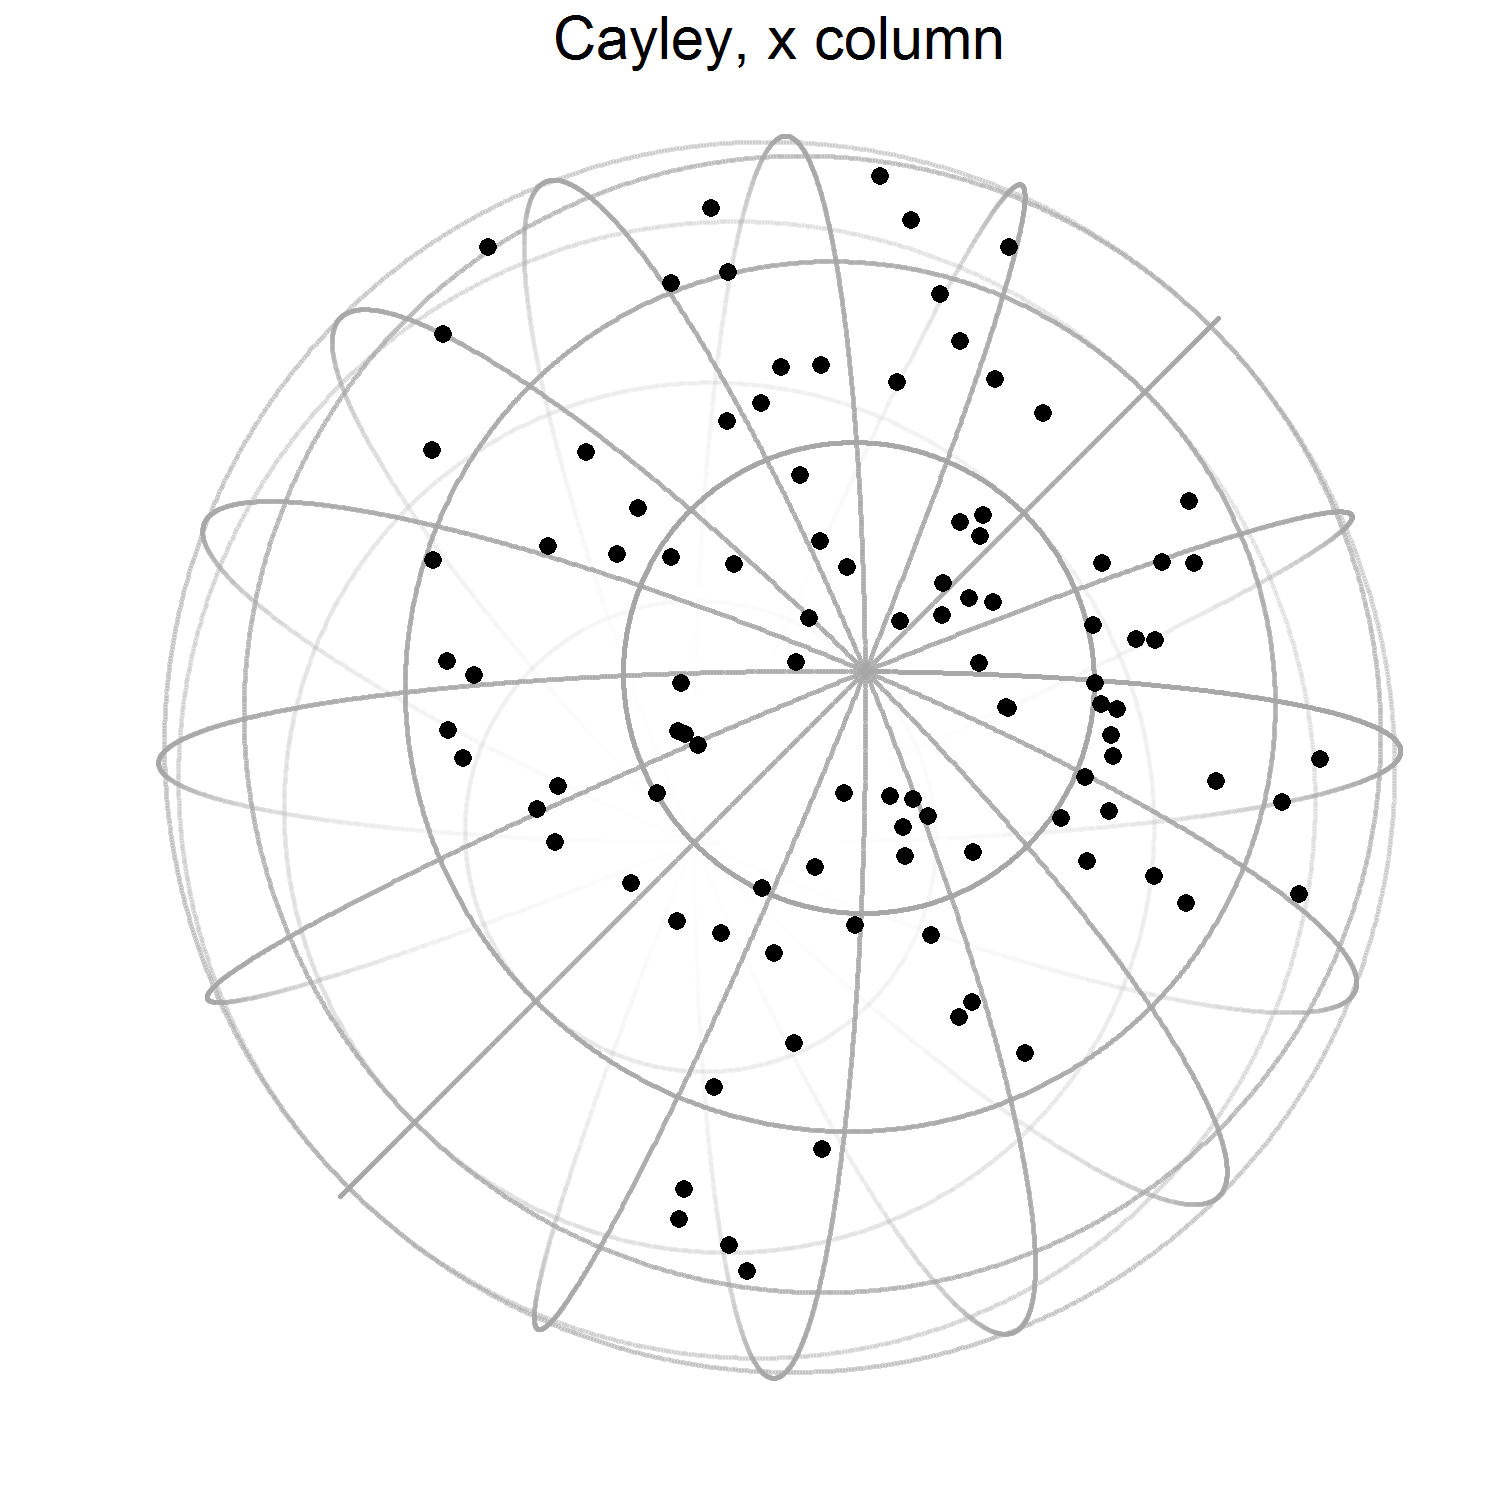
\includegraphics[width=.3\linewidth]{eye-cayley}
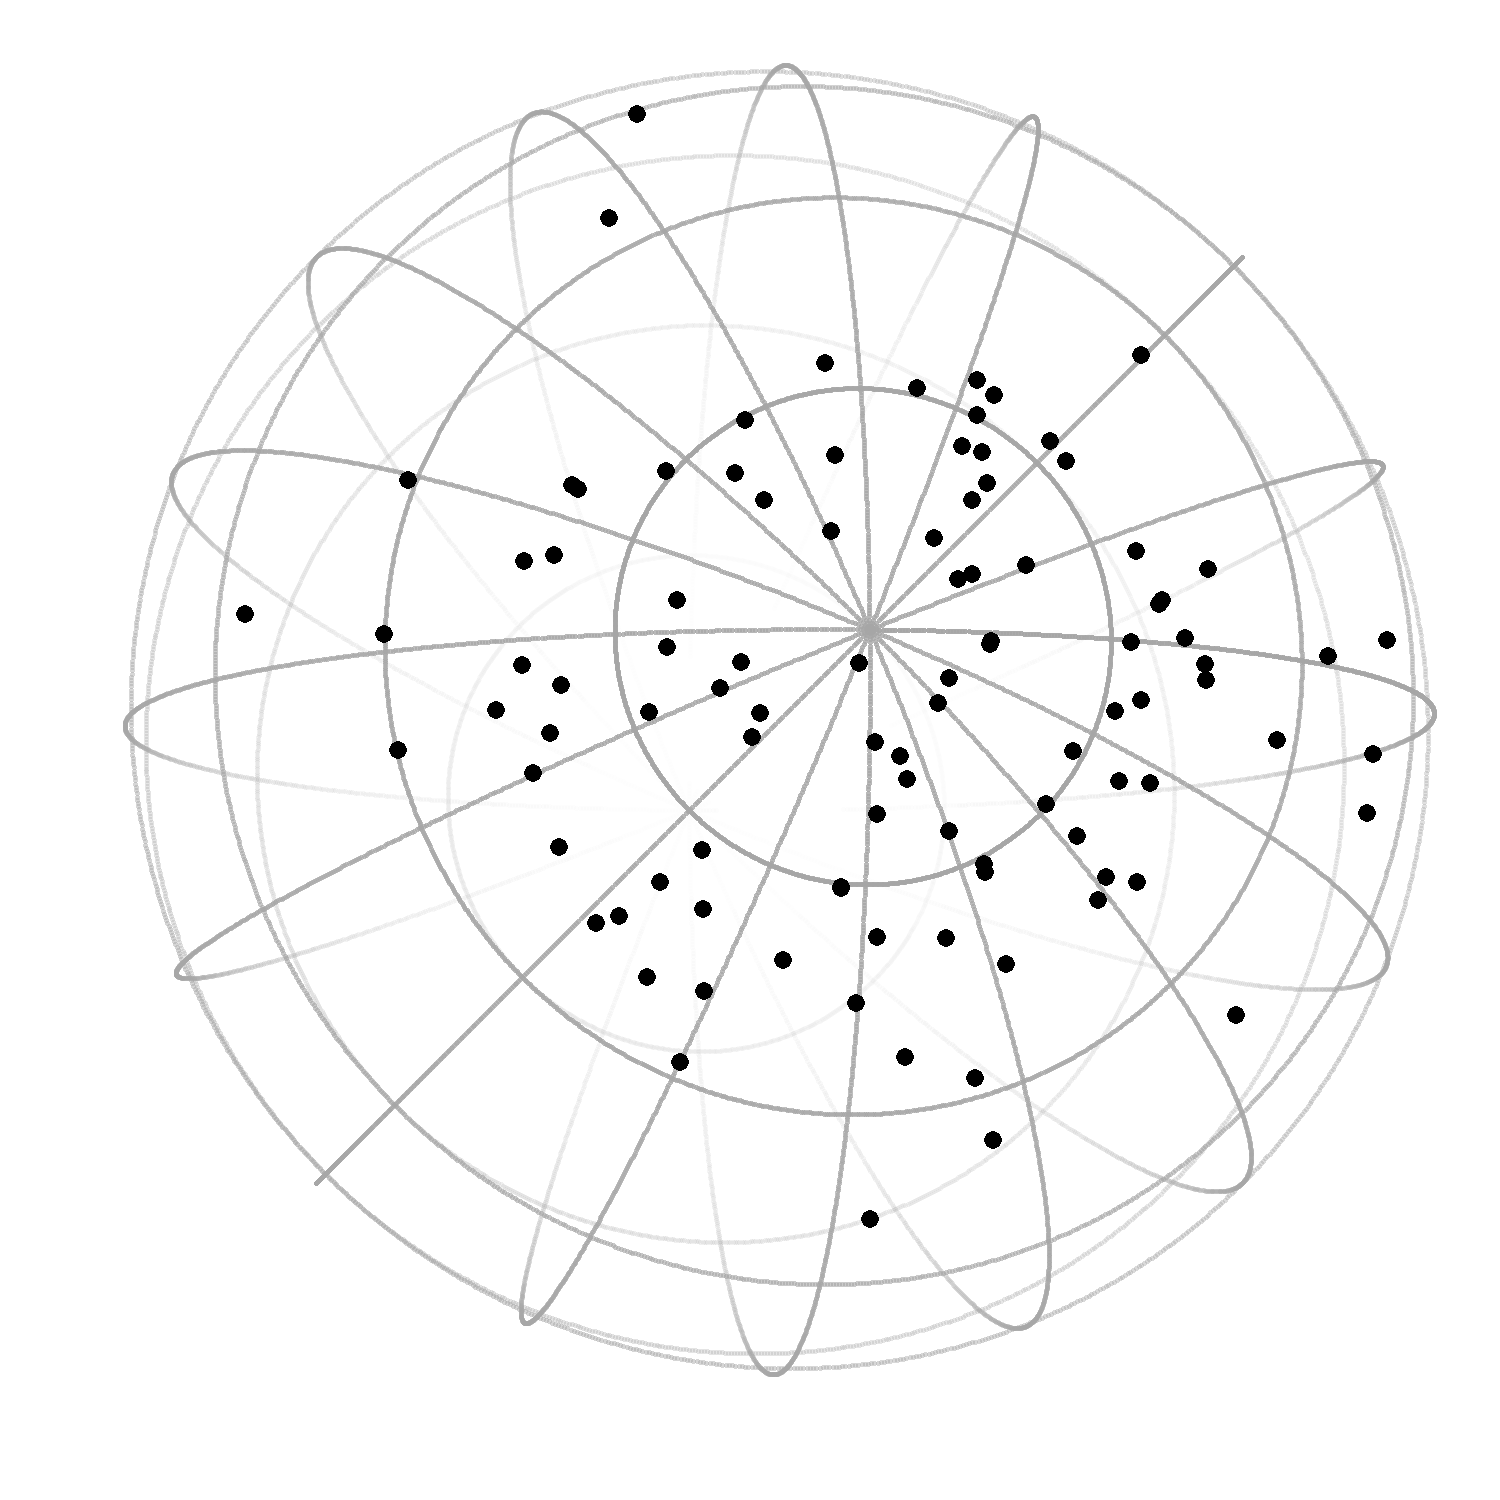
\includegraphics[width=.3\linewidth]{eye-cayley-2}
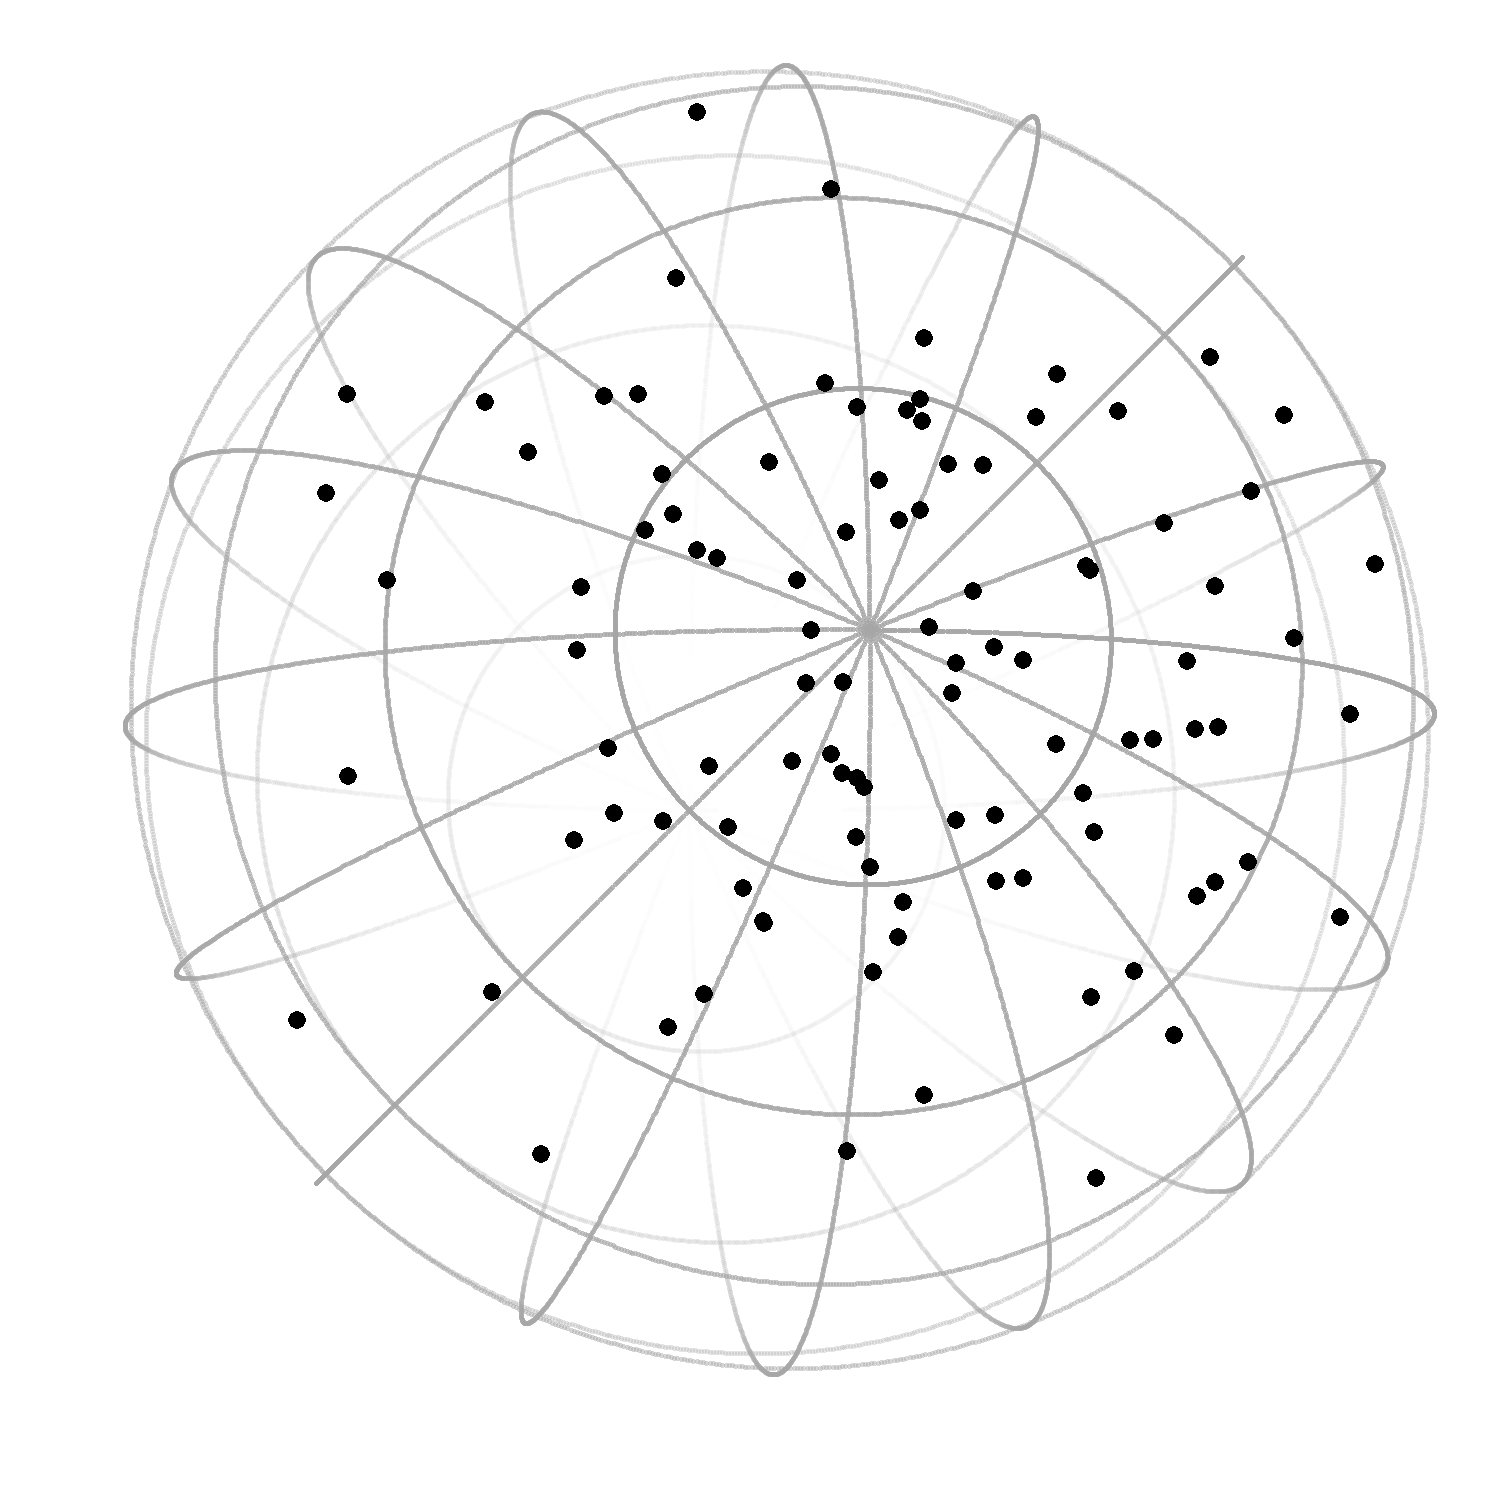
\includegraphics[width=.3\linewidth]{eye-cayley-3}
\caption{\label{fig:eye-cayley}Sphere plots for a sample of 100 rotations from a Cayley distribution with circular variance $\nu=0.25$}
\end{figure}
\begin{figure}
\centering
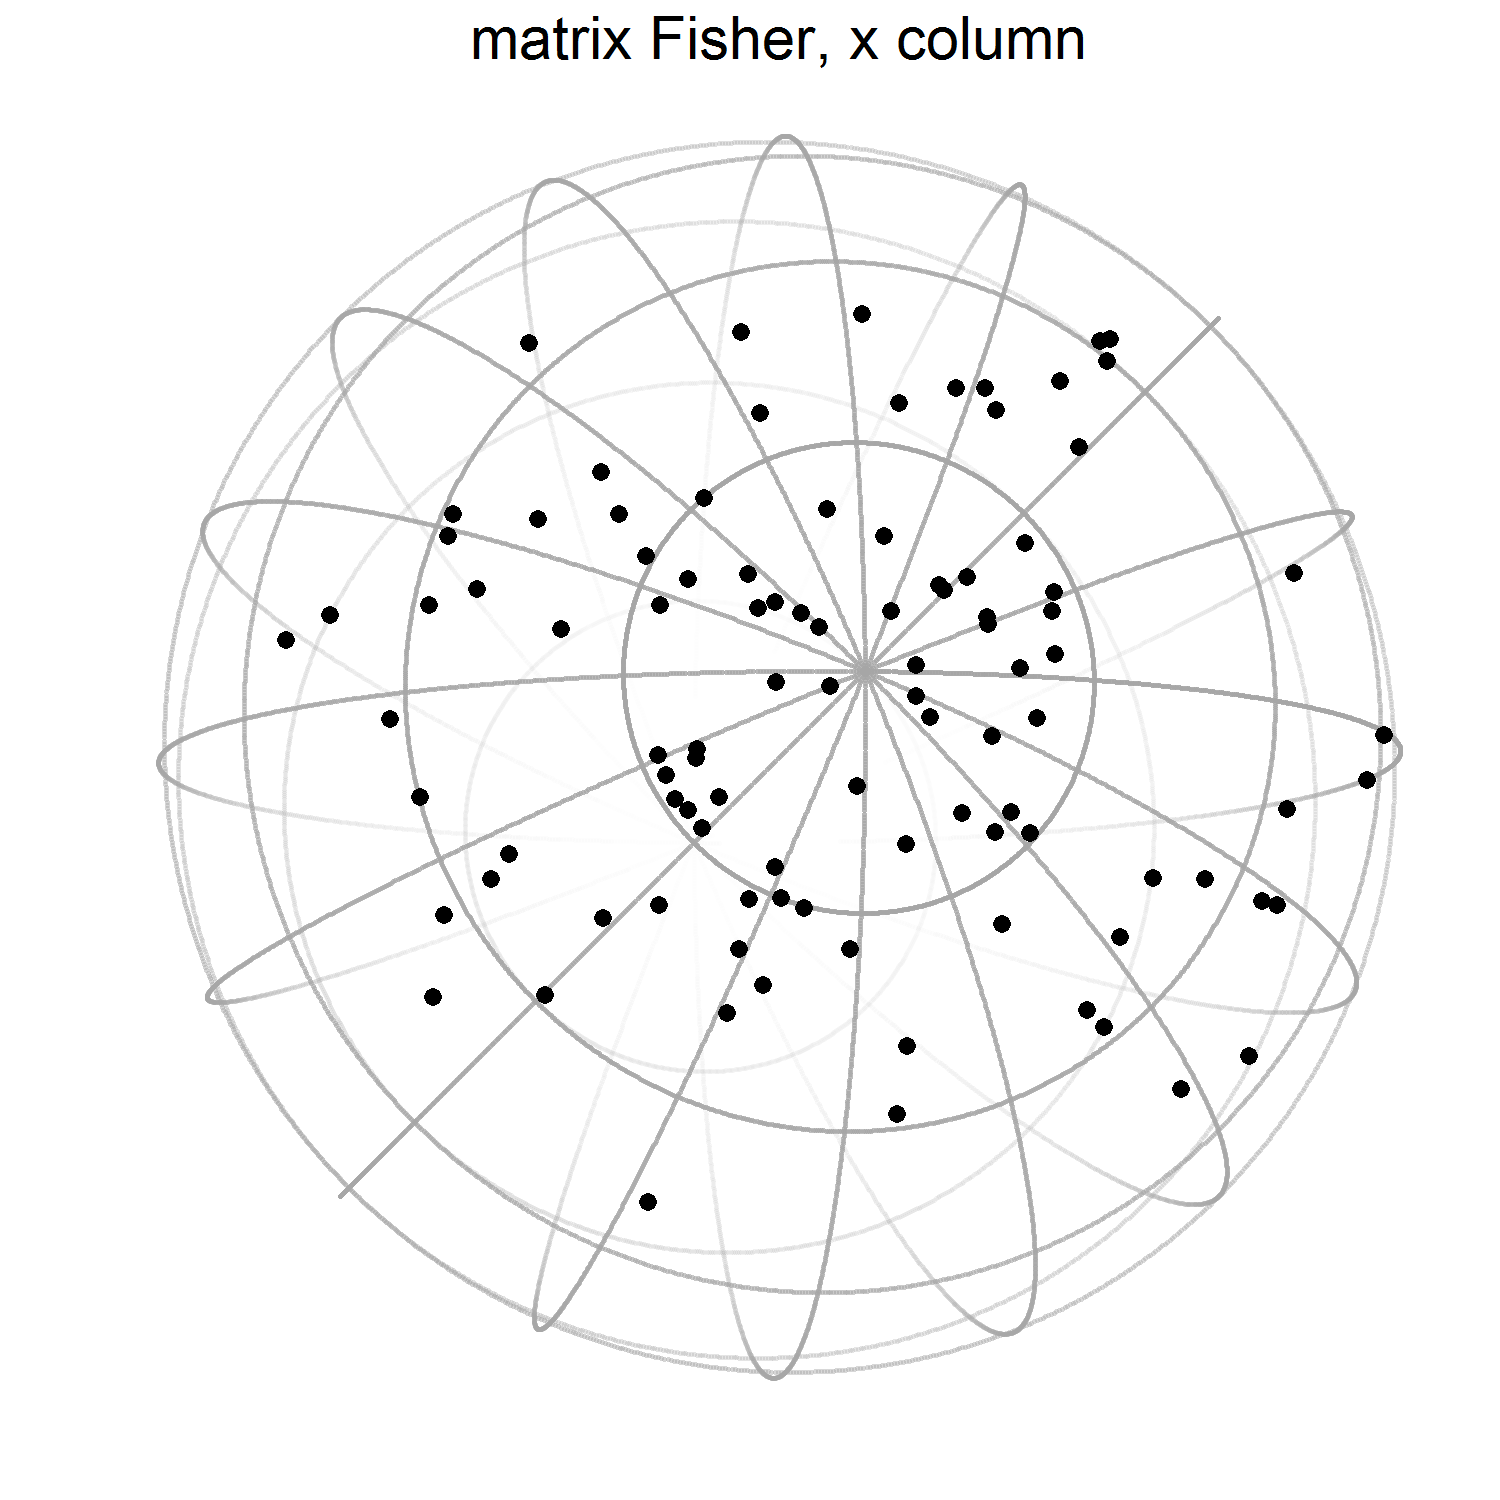
\includegraphics[width=.3\linewidth]{eye-fisher}
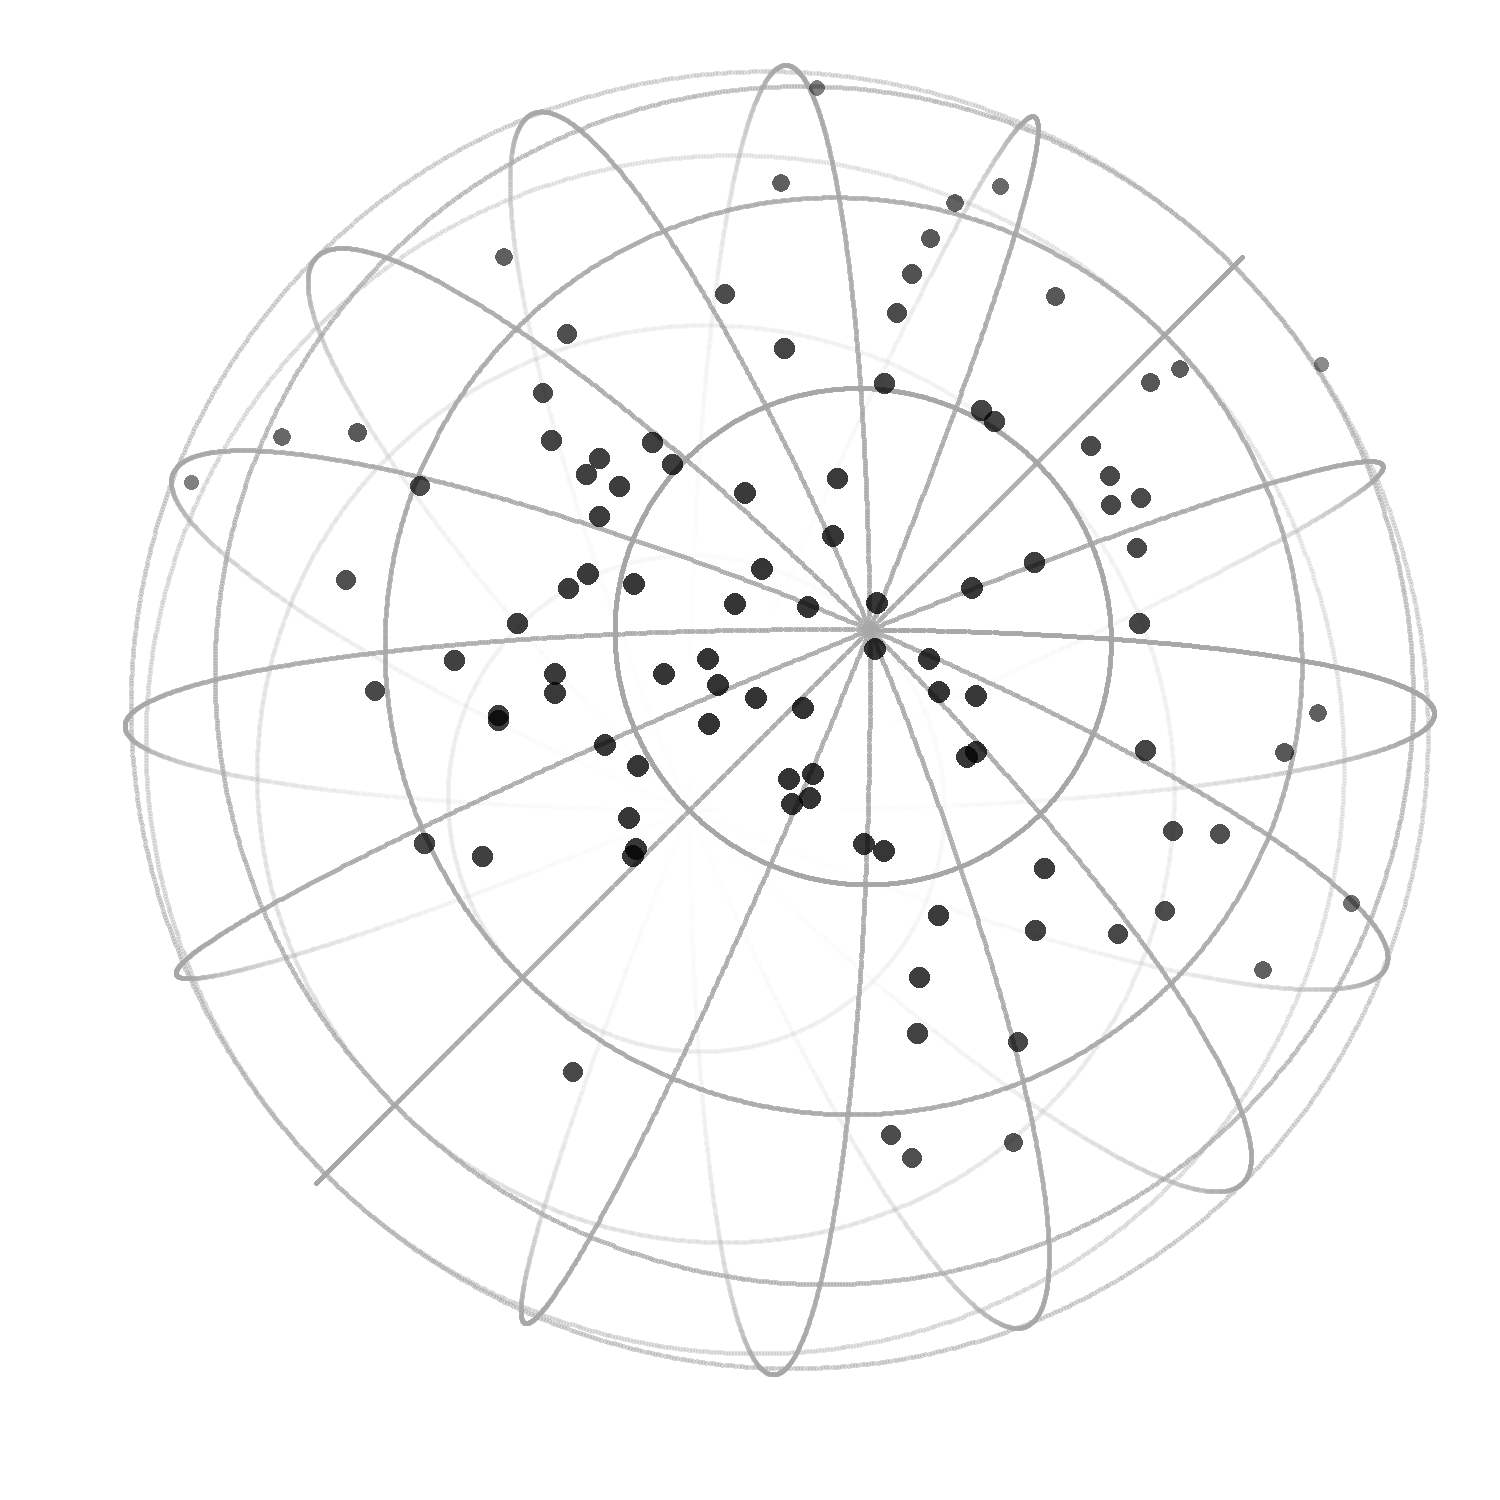
\includegraphics[width=.3\linewidth]{eye-fisher-2}
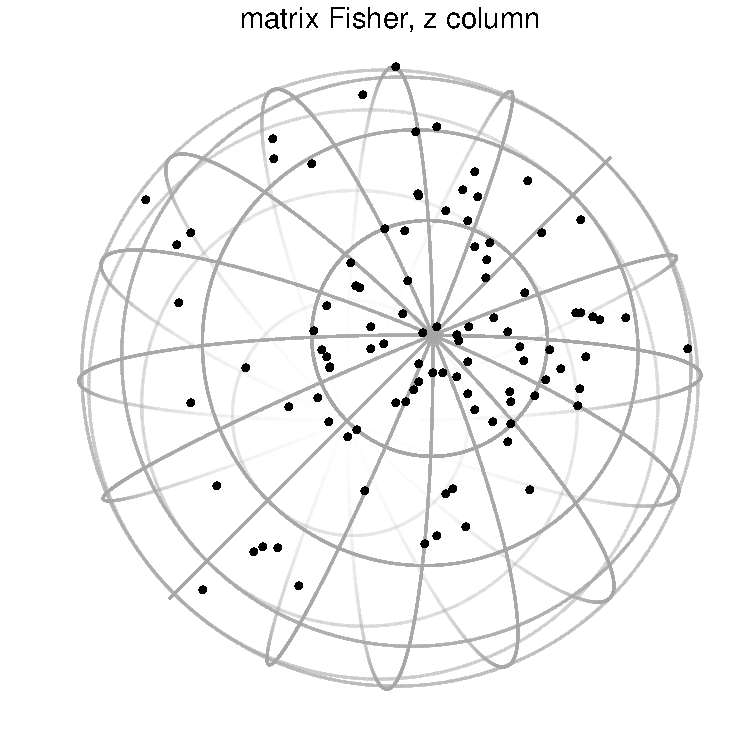
\includegraphics[width=.3\linewidth]{eye-fisher-3}
\caption{\label{fig:eye-fisher}Sphere plots for a sample of 100 rotations from a matrix Fisher distribution with circular variance $\nu=0.25$}
\end{figure}
\begin{figure}
\centering
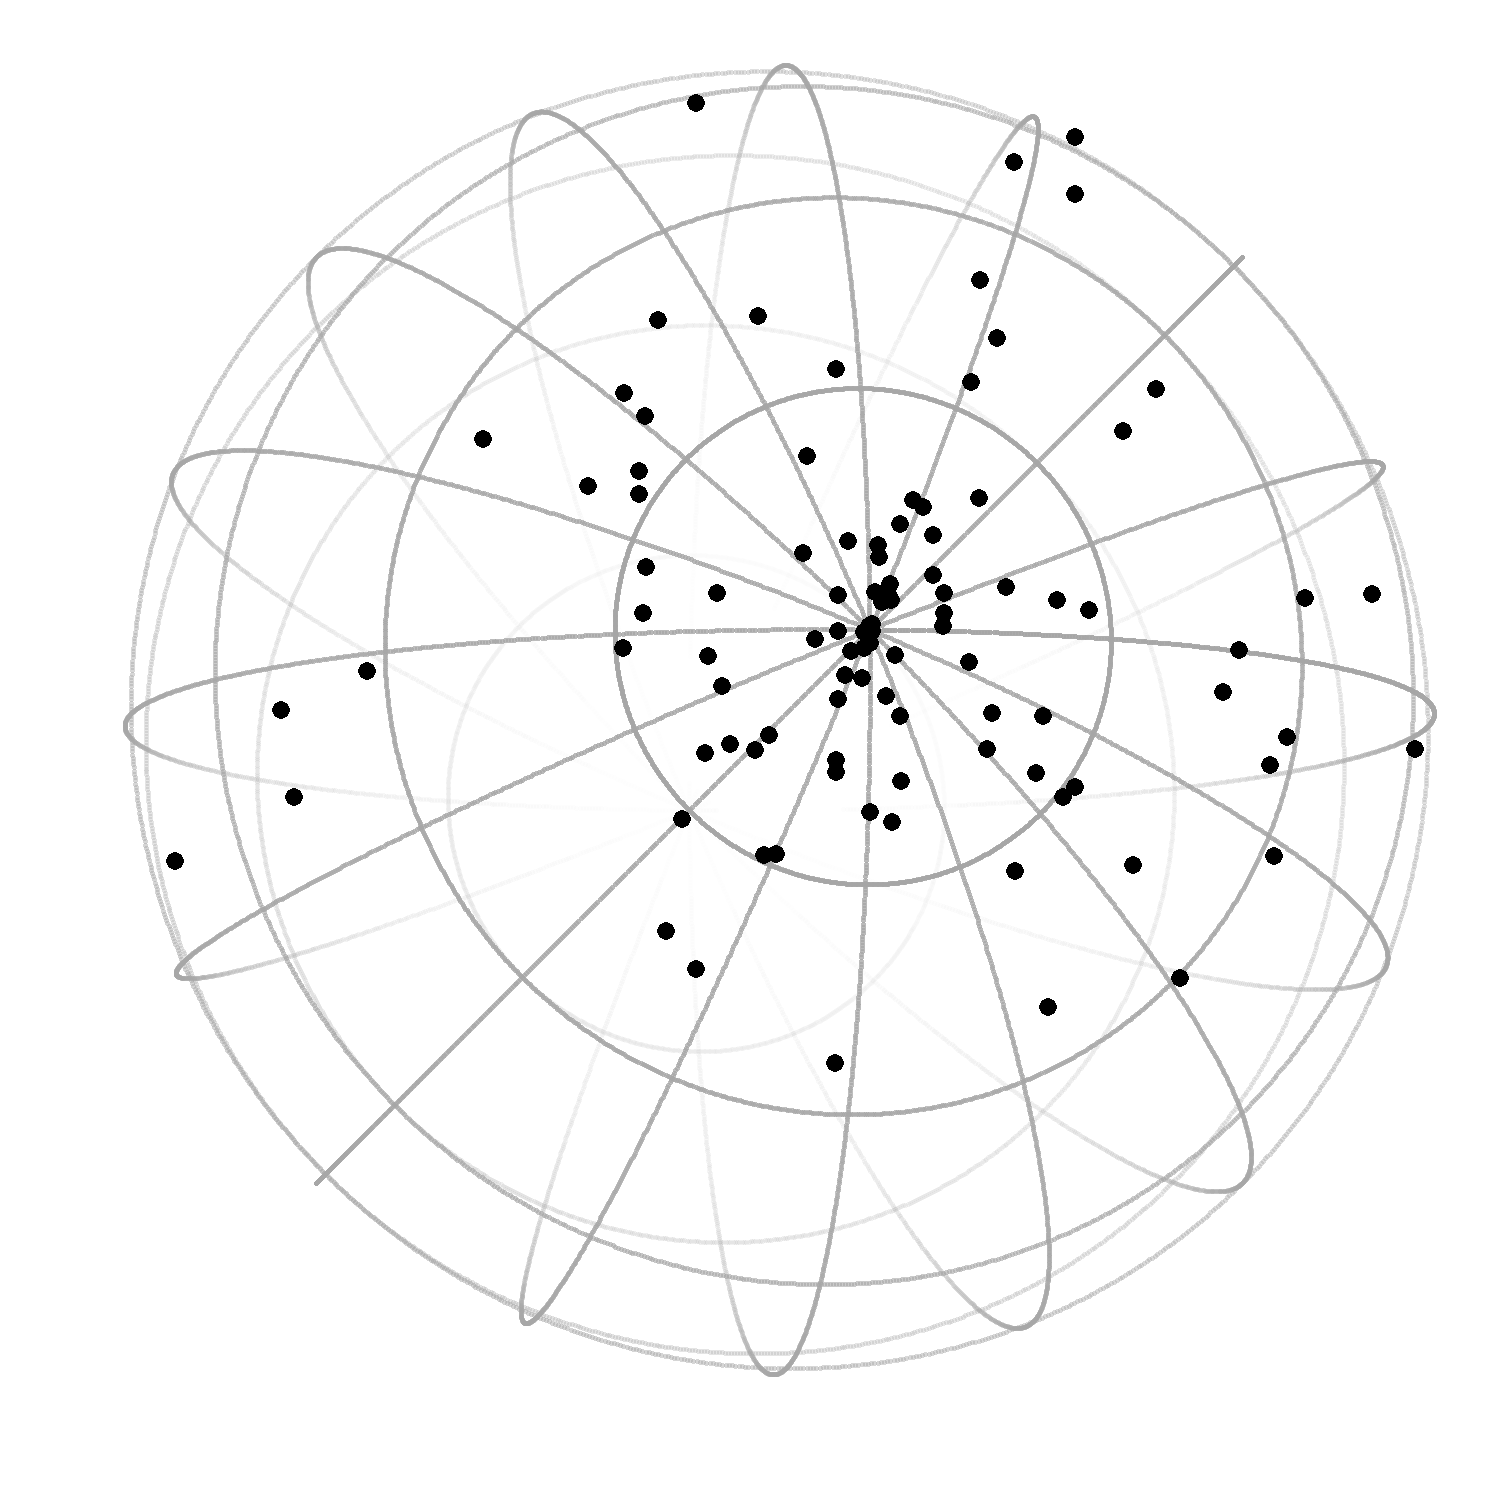
\includegraphics[width=.3\linewidth]{eye-vmises}
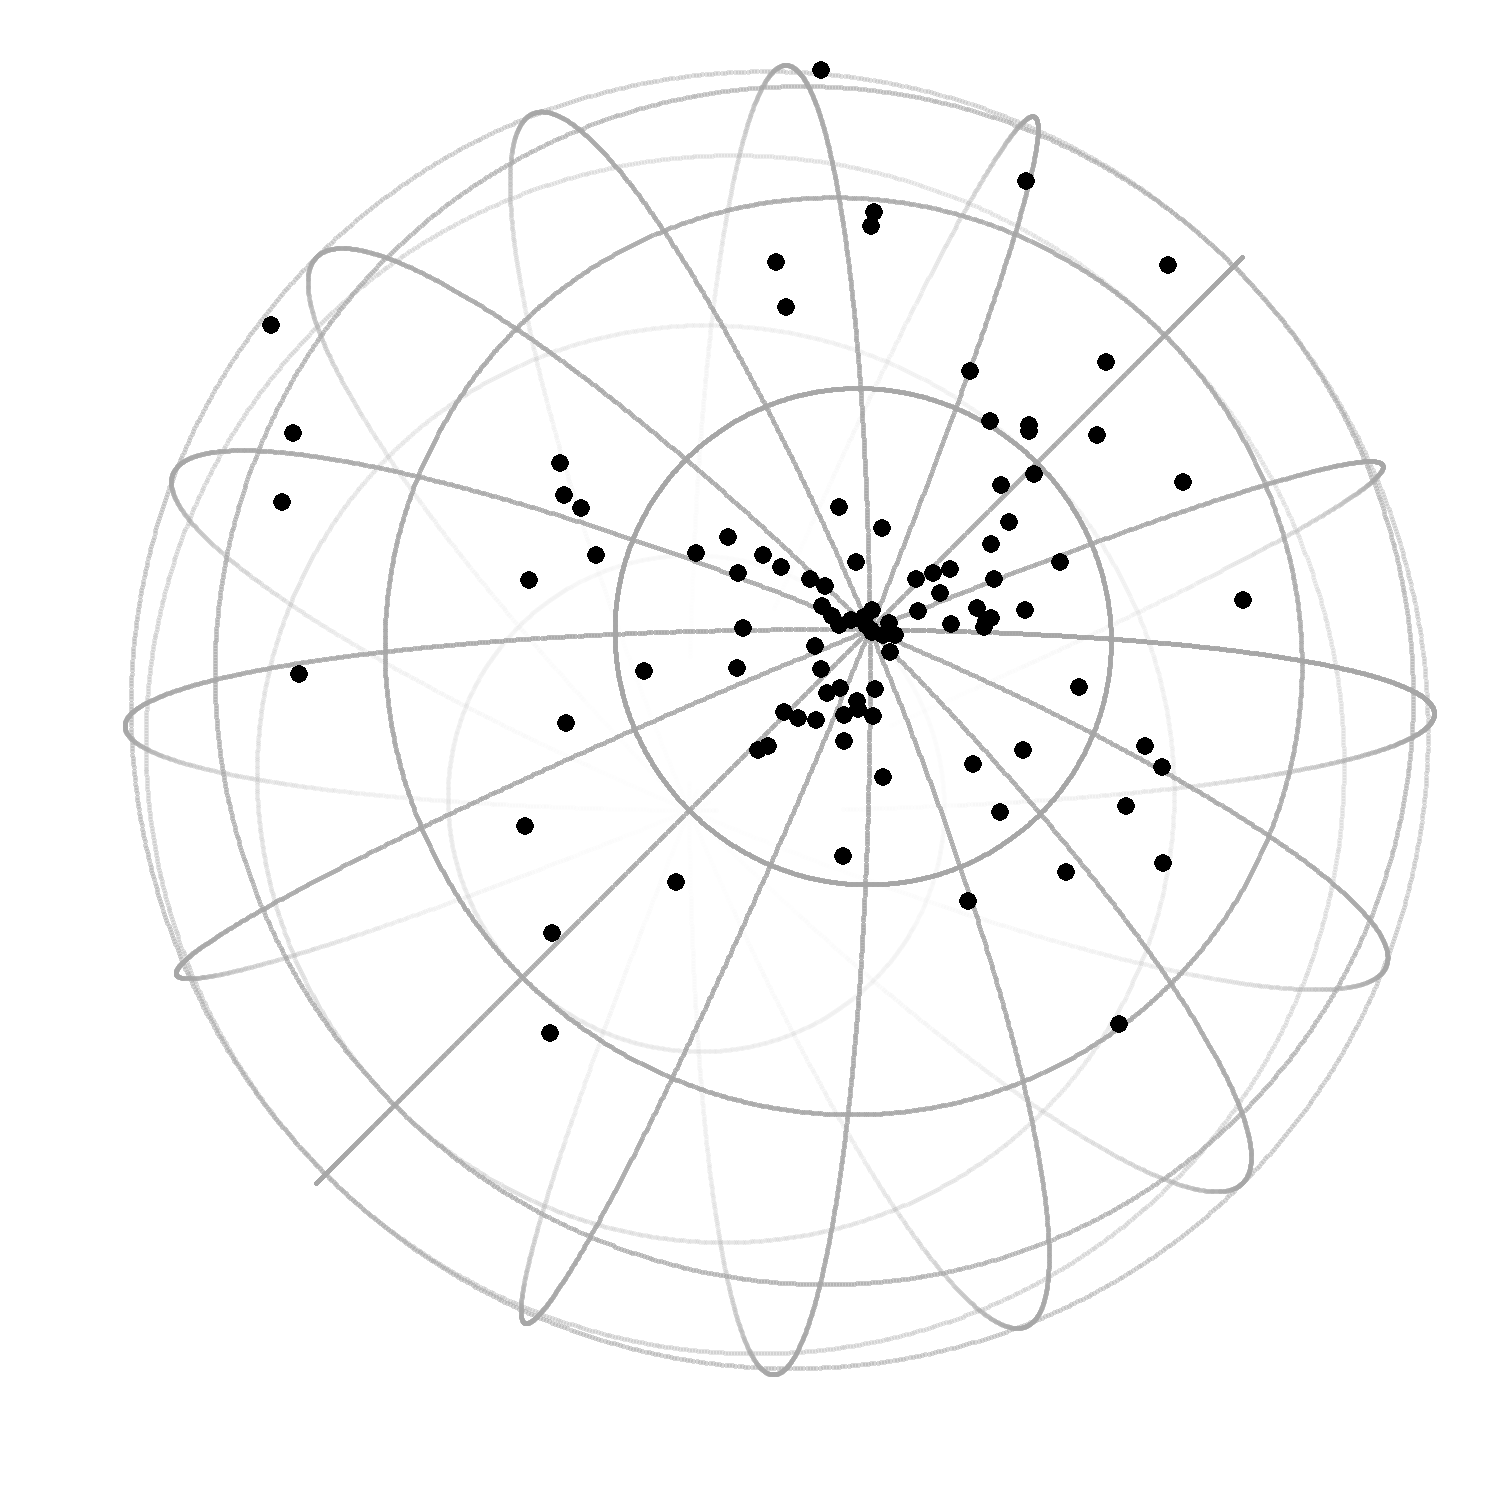
\includegraphics[width=.3\linewidth]{eye-vmises-2}
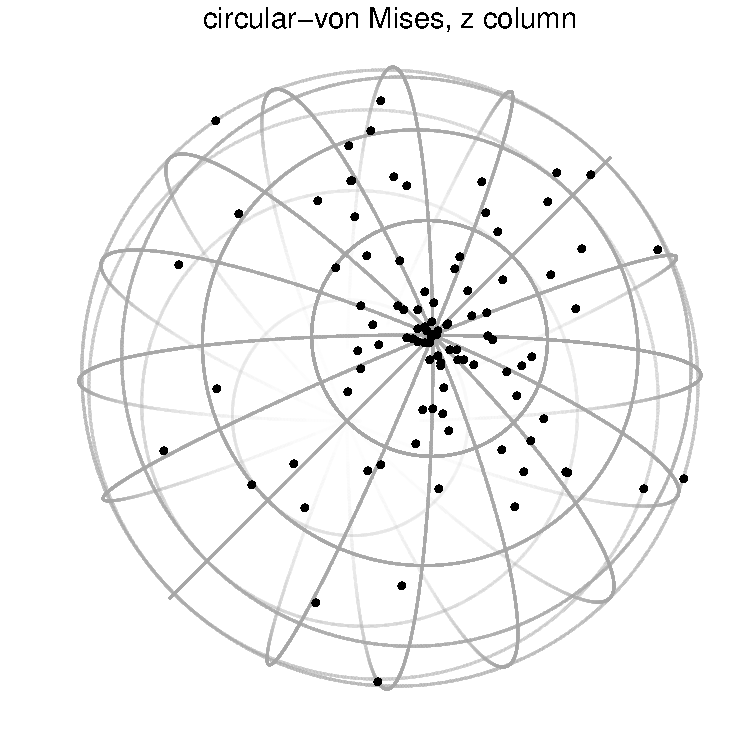
\includegraphics[width=.3\linewidth]{eye-vmises-3}
\caption{\label{fig:eye-vmises}Sphere plots for a sample of 100 rotations from a circular-von Mises distribution with circular variance $\nu=0.25$}
\end{figure}
\end{document}
\end{document}

